\documentclass[dvipsnames, svgnames, x11names]{beamer}
% \special{dvipdfmx:config z 0} %取消PDF压缩，加快速度，最终版本生成的时候最好把这句话注释掉
\usetheme{mytheme}
\usetikzlibrary{tikzmark}

% meta-data
\title{第三章}
\subtitle{农业数字化技术}
\author{张斌}
\institute[理工系]{河北农业大学 理工系}
\date{\the\year 年 \the\month 月}


% document body
\begin{document}
  
\begin{frame}
  \titlepage
  \thispagestyle{empty}
  \addtocounter{framenumber}{-1}
\end{frame}

\begin{frame}
    \frametitle{数字化}
    \highlight{数字技术} (Digital Technology) 是指借助一定的设备将各种信息，包括：图、文、声、像等，转化为电子计算机能识别的二进制数字，以及对数字信号进行运算、加工、存储、传送、利用的技术。
  \bigskip

  \highlight{数字化}是将模拟信号转变为数字信号的过程。是把模拟量转换为数字量的过程。

\end{frame}

\begin{frame}{}
  \begin{center}
      {\Huge \cbf{目 \ 录}}
  \end{center}
  \tableofcontents[subsectionstyle=hide/hide/show]
  \thispagestyle{empty}
  \addtocounter{framenumber}{-1}
\end{frame}

\section{模拟信号与数字信号}

\begin{frame}
    \frametitle{模拟信号}
        \begin{minipage}{0.48\linewidth}
            \highlight{模拟信号}是指用连续变化的物理量所表达的信息，如温度、湿度、压力、长度、电流、电压等等。实际生产生活中的各种物理量都是模拟信号。

    我们通常又把模拟信号称为\highlight{连续信号}，其信号的幅度，或频率，或相位随时间作连续变化，或在一段连续的时间间隔内，其代表信息的特征量可以在任意瞬间呈现为任意数值的信号。

    % 模拟信号传输过程中，先把信息信号转换成几乎“一模一样”的波动电信号(因此叫“模拟”)，再通过有线或无线的方式传输出去，电信号被接收下来后，通过接收设备还原成信息信号。
        \end{minipage}\hfill        
        \begin{minipage}{0.48\linewidth}
            \begin{center}
                \begin{tikzpicture}[scale=0.5]
                    \draw [->] (0,0) -- (13,0);
                    \draw [->] (0,0) -- (0,5);
                    \node at (0,0) [below] {0};
                    \node at (13,0) [below] {$t$};
                    \node at (0,5) [left] {$u$};
                    \draw[domain=0:12.56,smooth] plot(\x,{2*sin(\x r)});
                \end{tikzpicture}
            \end{center}
        \end{minipage}
    

\end{frame}

\begin{frame}
    \frametitle{模拟信号的优点}
    \begin{itemize}
      \item \cbf{精确的分辨率}
      
      在理想情况下，它具有无穷大的分辨率。与数字信号相比，模拟信号的信息密度更高。由于不存在量化误差，它可以对自然界物理量的真实值进行尽可能逼近的描述。

      \item \cbf{处理简单}
      
      当达到相同的效果，模拟信号处理比数字信号处理更简单。模拟信号的处理可以直接通过模拟电路组件（例如运算放大器等）实现，而数字信号处理往往涉及复杂的算法，甚至需要专门的数字信号处理器。
    \end{itemize}
\end{frame}

\begin{frame}
    \frametitle{模拟信号的缺点}
    \begin{minipage}{0.58\linewidth}
        近百年以来，无论是有线相连的电话，还是无线发送的广播电视，很长的时间内都是用模拟信号来传递信号的。照说模拟信号同原始信号在波形上几乎“一模一样”，似乎应该达到很好的传播效果，然而事实恰恰相反，这是因为信号在传输过程中要经过许多的处理和转送，产生各种干扰。

    模拟信号的主要缺点是它总是受到杂讯的影响。信号被多次复制，或进行长距离传输之后，这些随机噪声的影响可能会变得十分显著。
    \end{minipage}\hfill
    \begin{minipage}{0.38\linewidth}
        \begin{figure}[htpb]
            \centering
            
\includegraphics[width=\linewidth]{images/我听不见}
        \end{figure}
    \end{minipage}
\end{frame}

\begin{frame}
    \frametitle{数字信号}
        \begin{minipage}{0.48\linewidth}
            \highlight{数字信号}是指用一组特殊的状态来描述信号，典型的就是当前用最为常见的二进制数字来表示的信号。

    数字信号与模拟信号不同，它的自变量是离散的、因变量也是离散的，这种信号的自变量用整数表示，因变量用有限数字中的一个数字来表示。

    在实际的数字信号传输中，通常是将一定范围的信息变化归类为状态0或状态1， 这种状态的设置大大提高了数字信号的抗噪声能力。
        \end{minipage}\hfill
        \begin{minipage}{0.5\linewidth}
            \begin{center}
                \begin{tikzpicture}[scale=0.5]
                    \draw [->] (0,0) -- (13,0);
                    \draw [->] (0,0) -- (0,5);
                    \node at (0,0) [below] {0};
                    \node at (13,0) [below] {$t$};
                    \node at (0,5) [left] {$u$};
                    \draw (2,0) rectangle (4,4);
                    \draw[shift = {(4,0)}] (2,0) rectangle (4,4);
                \end{tikzpicture}
            \end{center}
        \end{minipage} 
\end{frame}

\begin{frame}
    \frametitle{数字信号的优点}
        \begin{minipage}{0.5\linewidth}
            \begin{itemize}
                \item 抗干扰能力强，无噪声积累
                \item 便于加密处理
                \item 便于储存、处理和交换
                \item 设备便于集成化、微型化
                \item 便于构建综合数字通信网
              \end{itemize}
        \end{minipage}\hfill
        \begin{minipage}{0.48\linewidth}
            \begin{figure}[htpb]
                \centering
                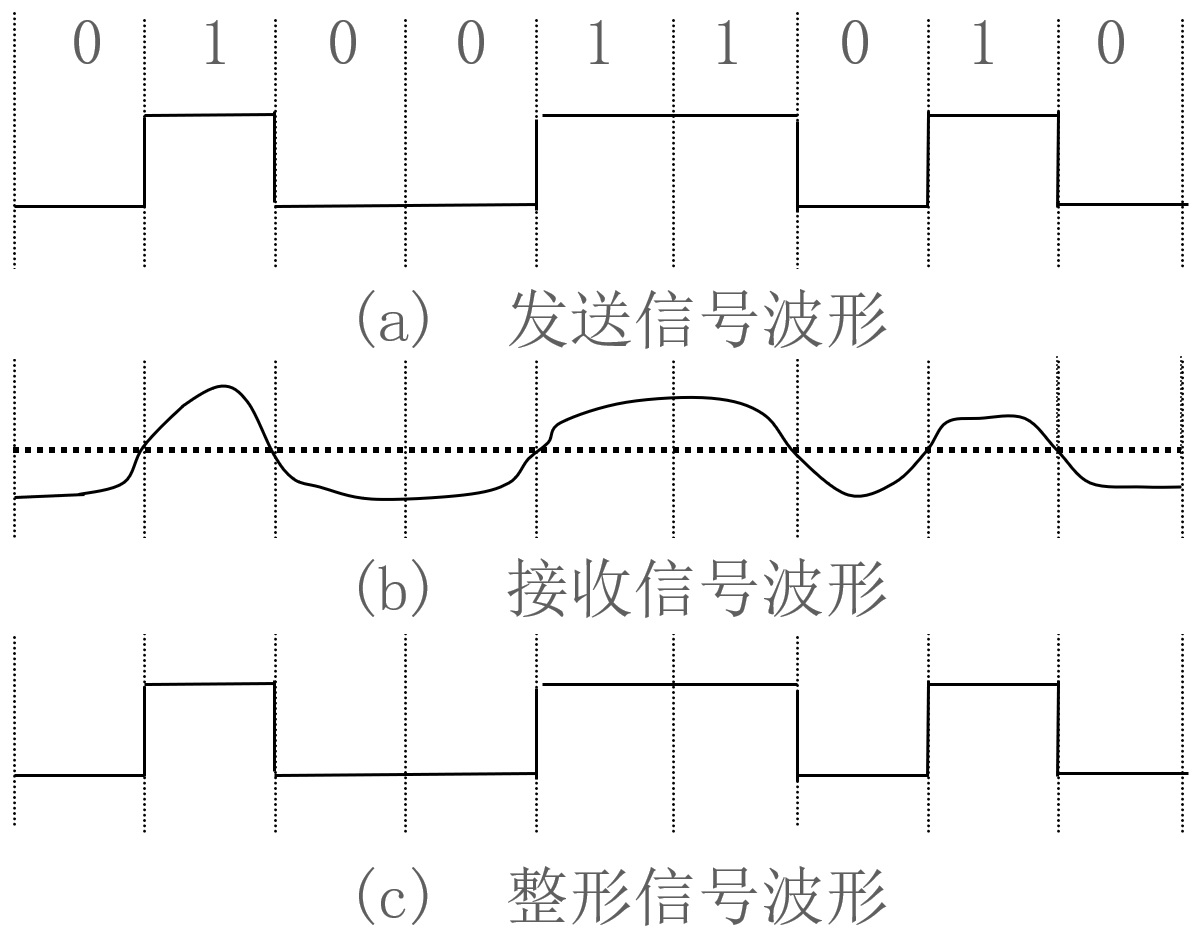
\includegraphics[width=\linewidth]{images/数字信号整形}
            \end{figure}
        \end{minipage}
\end{frame}


\begin{frame}
    \frametitle{数字信号的缺点}
    \begin{itemize}
      \item 增加了系统的复杂性
      \item 占用频带较宽，信号频率高
      \item 系统的功率消耗比较大
      \item 进行模/数转换时会带来量化误差
    \end{itemize}
\end{frame}

\begin{frame}
    \frametitle{模拟信号转换为数字信号}
        \begin{minipage}{0.48\linewidth}
            \begin{enumerate}
                \item \cbf{采样}
                
                把模拟信号由时间上连续变为时间上离散的。
                \item \cbf{量化}
                
                采样完了的信号时间上是离散的，间隔了若干周期才变化。但是因变量的取值仍然是随意的。那么在接下来的过程中，通过把这些因变量映射到固定的数值上去。
                \item \cbf{编码}
                
                以特定的二进制数值系统表征。
              \end{enumerate}
        \end{minipage}\hfill
        \begin{minipage}{0.5\linewidth}
            \begin{center}

                \only<1>{
                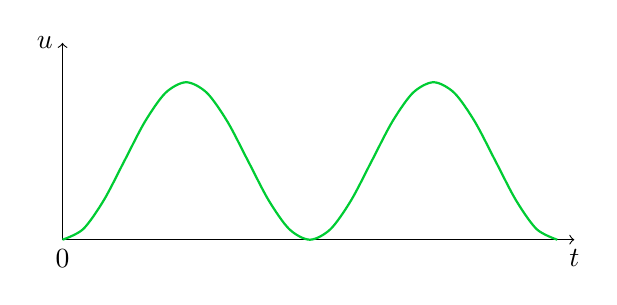
\begin{tikzpicture}[scale=0.5]
                    \draw [->] (0,0) -- (13,0);
                    \draw [->] (0,0) -- (0,5);
                    \node at (0,0) [below] {0};
                    \node at (13,0) [below] {$t$};
                    \node at (0,5) [left] {$u$};
                    \draw[domain=0:4*pi,smooth,thick,blue!20!green] plot(\x ,{2*sin((\x-pi/2) r)+2});
                \end{tikzpicture}
                }

                \only<2>{
                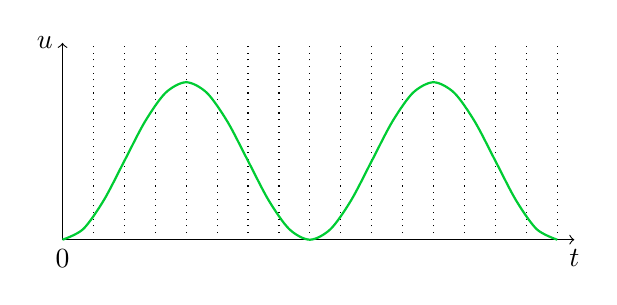
\begin{tikzpicture}[scale=0.5]
                    \draw [->] (0,0) -- (13,0);
                    \draw [->] (0,0) -- (0,5);
                    \foreach \x in {pi/4,2*pi/4,3*pi/4,4*pi/4,5*pi/4,6*pi/4,7*pi/4,8*pi/4,9*pi/4,10*pi/4,11*pi/4,12*pi/4,13*pi/4,14*pi/4,15*pi/4,16*pi/4}
                    \draw [dotted] (\x,0) -- (\x,5);
                    \node at (0,0) [below] {0};
                    \node at (13,0) [below] {$t$};
                    \node at (0,5) [left] {$u$};
                    \draw[domain=0:4*pi,smooth,thick,blue!20!green] plot(\x ,{2*sin((\x-pi/2) r)+2});
                \end{tikzpicture}
                }

                \only<3>{
                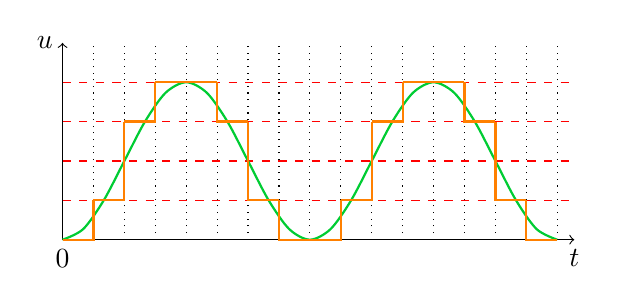
\begin{tikzpicture}[scale=0.5]
                    \draw [->] (0,0) -- (13,0);
                    \draw [->] (0,0) -- (0,5);
                    \foreach \x in {pi/4,2*pi/4,3*pi/4,4*pi/4,5*pi/4,6*pi/4,7*pi/4,8*pi/4,9*pi/4,10*pi/4,11*pi/4,12*pi/4,13*pi/4,14*pi/4,15*pi/4,16*pi/4}
                    \draw [dotted] (\x,0) -- (\x,5);
                    \foreach \x in {1,2,3,4}
                    \draw [red,dashed] (0,\x) -- (13,\x);
                    \node at (0,0) [below] {0};
                    \node at (13,0) [below] {$t$};
                    \node at (0,5) [left] {$u$};
                    \draw[domain=0:4*pi,smooth,thick,blue!20!green] plot(\x ,{2*sin((\x-pi/2) r)+2});
                    \draw[thick,orange] (0,0) -| (pi/4,1);
                    \draw[thick,orange] (pi/4,1) -| (pi/2,3);
                    \draw[thick,orange] (pi/2,3) -| (3*pi/4,4);
                    \draw[thick,orange] (3*pi/4,4) -| (5*pi/4,4);
                    \draw[thick,orange] (5*pi/4,4) |- (6*pi/4,3);
                    \draw[thick,orange] (6*pi/4,3) |- (7*pi/4,1);
                    \draw[thick,orange] (7*pi/4,1) |- (2*pi,0);
                    \draw[thick,orange,shift={(2*pi,0)}] (0,0) -| (pi/4,1);
                    \draw[thick,orange,shift={(2*pi,0)}] (pi/4,1) -| (pi/2,3);
                    \draw[thick,orange,shift={(2*pi,0)}] (pi/2,3) -| (3*pi/4,4);
                    \draw[thick,orange,shift={(2*pi,0)}] (3*pi/4,4) -| (5*pi/4,4);
                    \draw[thick,orange,shift={(2*pi,0)}] (5*pi/4,4) |- (6*pi/4,3);
                    \draw[thick,orange,shift={(2*pi,0)}] (6*pi/4,3) |- (7*pi/4,1);
                    \draw[thick,orange,shift={(2*pi,0)}] (7*pi/4,1) |- (2*pi,0);
                \end{tikzpicture}
                }
            \end{center}
        \end{minipage}
\end{frame}


\begin{frame}[t]
    \frametitle{}
    \begin{question}
        能不能不断提高采样率和量化位数，使数字音频的质量达到模拟声音的质量？
        \tcblower
        \pause
        从原理上讲通过不断提高采样率和量化位数来提高数字音频的质量是可行的。

        但是实际生活中：
        \begin{enumerate}
          \item 这样会大大增加保存信息的数据量以及信息处理量
          \item 我们的耳朵分辨能力也是有限的，过高的采样率和量化位数会造成浪费
        \end{enumerate}
        
    \end{question}
\end{frame}
\section{传感器}

\begin{frame}
    \frametitle{传感}
    如果我们要对自然界的信号加以记录和处理，我们应该是先把这些信号转变为电信号。这个转换的过程就叫做“\highlight{传感}”。

    执行这个过程的器件叫做\highlight{传感器}。传感器把某种物理量转变成了以电压或者电流表示的信号。

    这个信号是对现实世界物理量的“复刻”或者说“再现”。

\end{frame}

\begin{frame}
    \frametitle{传感器}
    传感器是将各种非电量（包括物理量、化学量、生物量等）按一定规律转换成便于处理和传输的另一种物理量（一般为电量）的装置。

传感器技术是利用各种功能材料实现信息检测的一门应用技术，它是检测（传感）原理、材料科学、工艺加工等三个要素的最佳结合。

传感原理是传感器工作时所依据的物理效应、化学反应和生物反应等机理，各种功能材料则是传感技术发展的物质基础，从某种意义上讲，传感器也就是能感知外界各种被测信号的功能材料。

\end{frame}

\begin{frame}
    \frametitle{传感器的组成}
    传感器（sensor）是由敏感元件和转换元件组成的一种检测装置，能感受到被测量，并能将检测和感受到的信息，按一定规律变换成为电信号（电压、电流、频率或相位）输出，以满足感知信息的传输、处理、存储、显示、记录和控制的要求。
    \bigskip

    \begin{center}
        \begin{tikzpicture}
            \draw[->] (0,0.5) -- (2,0.5) node [above,midway] {被测信息};
            \draw (2,0) rectangle (4,1) node [midway] {敏感元件};
            \draw[->,shift={(4,0)}] (0,0.5) -- (2,0.5);
            \draw[shift={(4,0)}] (2,0) rectangle (4,1) node [midway] {转换元件};
            \draw[->,shift={(8,0)}] (0,0.5) -- (2,0.5);
            \draw[shift={(8,0)}] (2,0) rectangle (5,1) node [midway] {信号调理电路};
            \draw[->,shift={(13,0)}] (0,0.5) -- (2,0.5) node [above,midway] {输出信息};
            \draw[->,shift={(7,0)}] (0,-1) -- (0,0);
            \draw[->,shift={(12.5,0)}] (0,-1) -- (0,0);
            \draw (6,-2) rectangle (13,-1) node [midway] {辅助电源电路};
        \end{tikzpicture}
    \end{center}
\end{frame}





\subsection{传感器的分类}

\begin{frame}
    \frametitle{按照测量对象进行分类}
        \begin{minipage}{0.25\linewidth}
            \begin{itemize}
                \item 温度传感器
                \item 压力传感器
                \item 位移传感器
                \item 速度传感器
                \item 湿度传感器
                \item 气体传感器
                \item $\cdots \cdots$
            \end{itemize}
        \end{minipage}\hfill
        \begin{minipage}{0.73\linewidth}
            \begin{figure}[htpb]
                \centering
                
\includegraphics[height=.3\textwidth]{images/温度湿度计}
                
\includegraphics[height=.3\textwidth]{images/可燃气体传感器}
                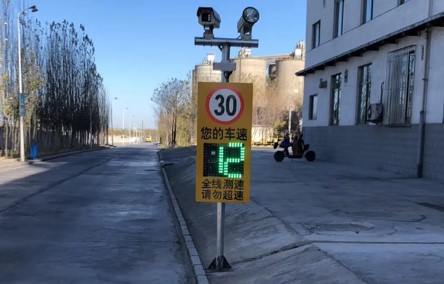
\includegraphics[height=.3\textwidth]{images/车速测量}
                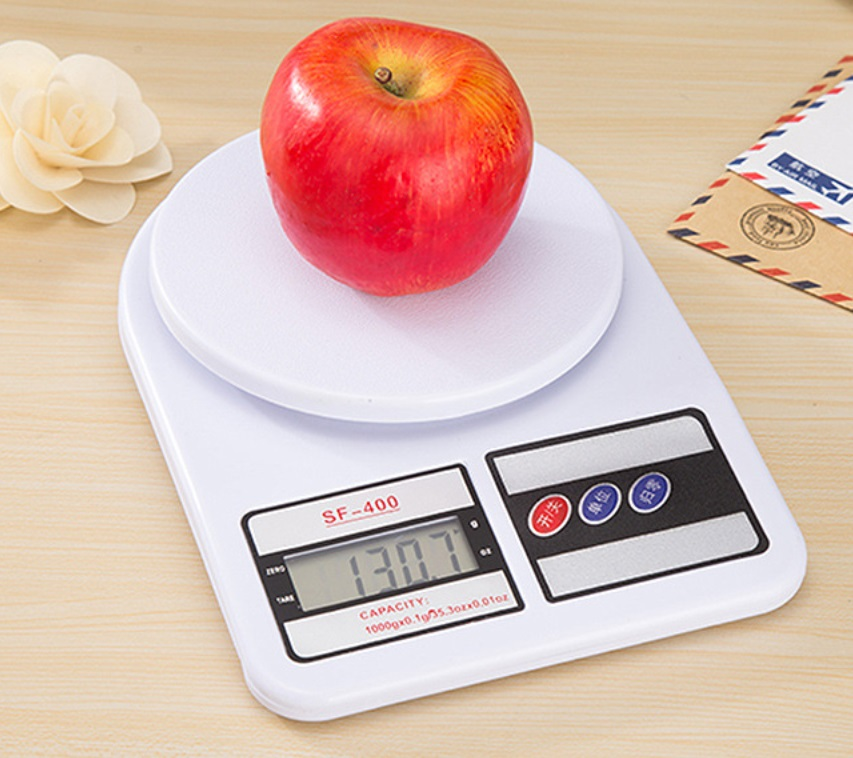
\includegraphics[width=.375\textwidth, height=.3\textwidth]{images/电子称.jpg}
            \end{figure}
        \end{minipage}
\end{frame}

\begin{frame}
    \frametitle{按照检测原理进行分类}
    \begin{itemize}
        \item {\cbf{物理传感器}}
        
        物理传感器是检测物理量的传感器。它是利用某些物理效应，把被测量的物理量转化成为便于处理的能量形式的信号的装置。

        如力传感器、声传感器、温度传感器、光传感器、电传感器、磁传感器、射线传感器
        \item {\cbf{化学传感器}}
        
        化学传感器是对各种化学物质敏感并将其浓度转换为电信号进行检测的仪器。
        \item {\cbf{生物传感器}}
        
        生物传感器是由生物敏感元件与信号转换器构成的分析装置。

        生物敏感元件的作用是识别目标物质，主要包括：抗体、酶、核酸、细胞等生物物质；也包括一些类似于生物物质的合成的物质。
    \end{itemize}
\end{frame}

\begin{frame}
    \frametitle{按照传感器的结构参数在信号变换过程中是否发生变化进行分类}
    \begin{itemize}
        \item {\cbf{物性型}}
        
        在实现信号的变换过程中，结构参数基本不变，而是依靠敏感元件材料本身物理或化学性质的变化来实现信号变换。例如利用水银的热胀冷缩现象制成水银温度计来测温；利用石英晶体的压电效应制成压电测力计等。

        \begin{itemize}
            \item 压阻式传感器（压阻效应，压阻系数改变）
            \item 光电式传感器（光电效应，光子轰击引起物体电阻率改变）
            \item 压电式传感器（压电效应，压力引起电动势改变）
            \item 热电式传感器（热电效应，温度引起电动势改变）
        \end{itemize}
        \item {\cbf{结构型}}
        
        依靠传感器结构参数的变化而将外界被测量参数转化成相应的电阻、电感、电容等物理量的变化，实现信号转换。
        \begin{itemize}
            \item 电容式传感器依靠极板间距离变化引起电容量变化；
            \item 电感式传感器依靠衔铁位移引起自感或互感变化等。
        \end{itemize}
        
    \end{itemize}
\end{frame}

\begin{frame}
    \frametitle{根据敏感元件与被测对象之间的能量关系进行分类}
    \begin{itemize}
        \item {\cbf{能量转换型}}
        
        该类传感器能将输入的非电能量转换成电能输出，传感器本身勿需外加电源，信号能量直接从被测对象取得。
        
        但由于这类传感器是被测对象与传感器之间的能量传输，必然导致被测对象状态的变化，而造成测量误差。

        \item {\cbf{能量控制型}}
        
        该类传感器在进行信号转换时，需要从外部供给辅助能源使传感器工作，并由被测量来控制外部供给能量的变化。通过测量电路将它变为电压或电流量，然后进行转换、放大，以推动指示或记录仪表。

        例如，电阻应变测量中，应变计接于电桥上，电桥工作能源由外部供给，而由于被测量变化所引起应变计的电阻变化来控制电桥的不平衡程度。
    \end{itemize}
\end{frame}


\begin{frame}
    \frametitle{自发电无线门铃\link{https://www.bilibili.com/video/av94579506}}
    \begin{figure}[htpb]
        \centering
        
\includegraphics[width=.7\linewidth]{门铃}
    \end{figure}
\end{frame}


\begin{frame}
    \frametitle{按输出信号的性质分类}
    \begin{itemize}
        \item {\cbf{模拟式传感器}}
        
        将被测非电量转换成连续变化的电压或电流。

        模拟传感器的模拟处理方式是连续的。一旦输入改变，输出也会改变。
        \item {\cbf{数字式传感器}}
        
        能直接将非电量转换为数字量，可以直接用于数字显示和计算，可直接配合计算机，具有抗干扰能力强，适宜距离传输等优点。

        数字传感器的数字处理方式是离散的。当输入更改时，系统会记录更改之前会存在延迟。此延迟的长度由“采样频率”决定，并由时钟控制。
    \end{itemize}
\end{frame}

\begin{frame}
    \frametitle{按照传感器与被测对象的关联方式进行分类}
    \begin{itemize}
        \item {\cbf{接触式}}
        
        必须接触才能有信号。如压力传感器，电位差计式传感器等。
        \item {\cbf{非接触式}}
        
        非接触化测量可以消除传感器介入而使被测量受到的影响，提高测量的准确性，同时，可使传感器的使用寿命增加。但是非接触式传感器的输出会受到被测对象与传感器之间介质或环境的影响。因此传感器标定必须在使用现场进行。例如红外测温枪、红外测温仪以及农业遥感、航空摄影均属于非接触式传感技术。
    \end{itemize}
\end{frame}

\begin{frame}
    \frametitle{按作用形式分类}
        \begin{minipage}{0.38\linewidth}
            \begin{itemize}
                \item {\cbf{主动型}}
                
                主动发出探测信号
                    \begin{itemize}
                        \item 激光雷达
                        \item 声纳
                    \end{itemize}
                \item {\cbf{被动型}}
                
                被动接收被测对象本身产生的信号
                \begin{itemize}
                    \item 红外辐射温度计
                    \item 红外摄像装置
                \end{itemize}
            \end{itemize}
        \end{minipage}\hfill
        \begin{minipage}{0.58\linewidth}
            \begin{figure}[htpb]
                \centering
                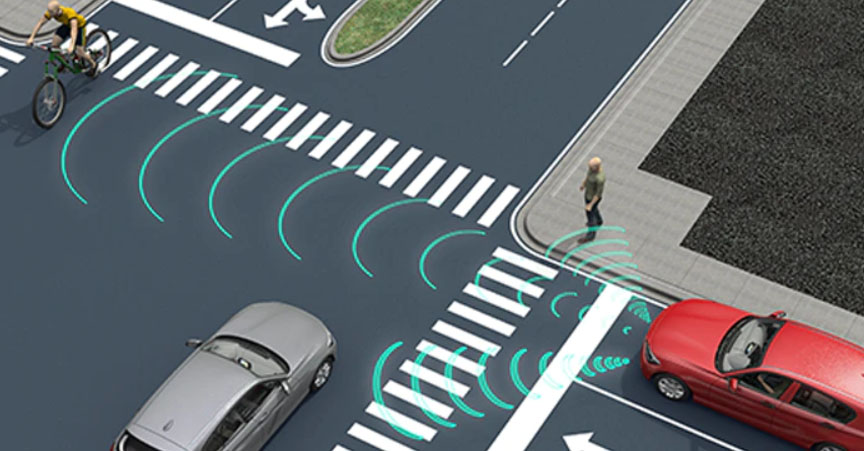
\includegraphics[width=\linewidth]{images/雷达}
            \end{figure}
        \end{minipage}
    
\end{frame}

\begin{frame}
    \frametitle{按传感器构成来分类}
    \begin{center}
        {\Large \cbf{“没有什么是一个传感器解决不了的”}}
        \bigskip

        {\Large \cbf{“如果有，就两个”}}
    \end{center}
    \begin{itemize}
      \item {\cbf{基本型传感器}}
      
      是一种最基本的单个变换装置
      \item {\cbf{组合型传感器}}
      
      是由不同单个变换装置组合而构成的传感器
      \item {\cbf{应用型传感器}}
      
      是基本型传感器或组合型传感器与其他机构组合而构成的传感器
    \end{itemize}
\end{frame}

\subsection{常用传感器}

\begin{frame}
    \frametitle{温度传感器}
    \begin{figure}[htpb]
        \centering
        
\includegraphics[height=.44\linewidth]{images/水银温度计.jpg}
        
\includegraphics[height=.44\linewidth]{images/耳温枪.jpg}
        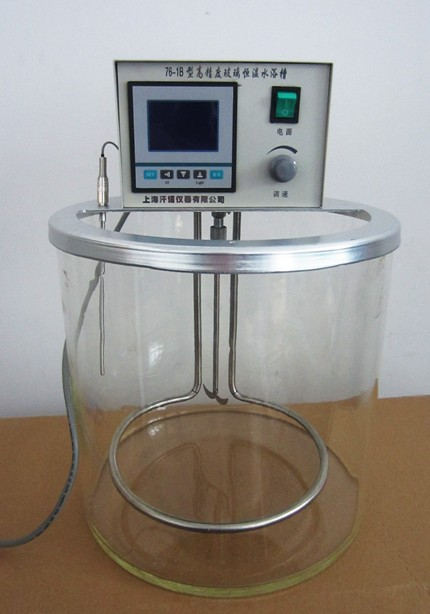
\includegraphics[height=.44\linewidth]{images/水浴锅.jpg}
    \end{figure}
\end{frame}

% 恒温水浴锅是利用传感器将水槽内水的温度转换为电阻值，输出控制信号，有效地控制电加热管的平均加热功率，使水槽内的水保持恒温。常作蒸发和恒温加热用，当被加热的物体要求受热均匀，温度不超过100℃时，可以用水浴加热。

\begin{frame}
    \frametitle{力传感器}
        \begin{minipage}{0.63\linewidth}
            \begin{figure}[htpb]
                \centering
                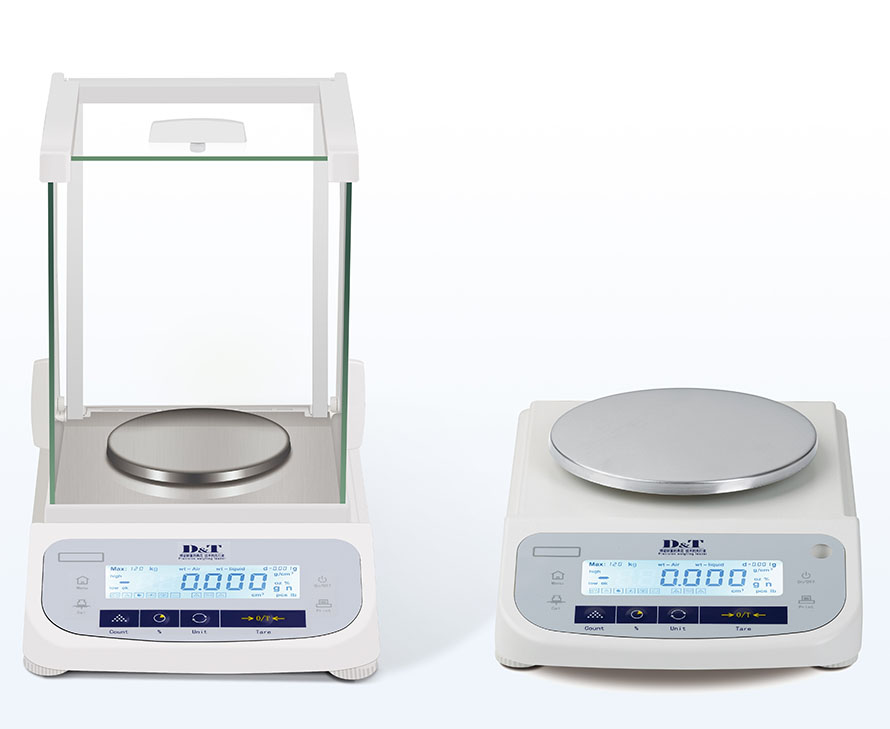
\includegraphics[height=200pt]{images/天平}
            \end{figure}
        \end{minipage}\hfill
        \begin{minipage}{0.35\linewidth}
            
            \begin{itemize}
                \item 压电式压力传感器
                \item 压阻式压力传感器
                \item 电容式压力传感器
              \end{itemize}
              \begin{figure}[htpb]
                \centering
                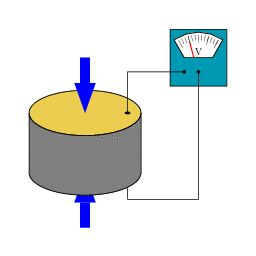
\includegraphics[width=.8\linewidth]{images/压力传感器.jpg}
            \end{figure}
        \end{minipage}
\end{frame}

% 一、压电压力传感器
% 压电式压力传感器大多是利用正压电效应制成的。正压电效应是指：当晶体受到某固定方向外力的作用时，内部就产生电极化现象，同时在某两个表面上产生符号相反的电荷；当外力撤去后，晶体又恢复到不带电的状态；当外力作用方向改变时，电荷的极性也随之改变；晶体受力所产生的电荷量与外力的大小成正比。
% 二、压阻压力传感器
% 压阻压力传感器主要基于压阻效应（Piezoresistive effect）。压阻效应是用来描述材料在受到机械式应力下所产生的电阻变化。不同于上述压电效应，压阻效应只产生阻抗变化，并不会产生电荷。
% 大多数金属材料与半导体材料都被发现具有压阻效应。其中半导体材料中的压阻效应远大于金属。
% 压阻压力传感器一般通过引线接入惠斯登电桥中。平时敏感芯体没有外加压力作用，电桥处于平衡状态（称为零位），当传感器受压后芯片电阻发生变化，电桥将失去平衡。若给电桥加一个恒定电流或电压电源，电桥将输出与压力对应的电压信号，这样传感器的电阻变化通过电桥转换成压力信号输出。
% 三、电容式压力传感器
% 电容式压力传感器是一种利用电容作为敏感元件，将被测压力转换成电容值改变的压力传感器。这种压力传感器一般采用圆形金属薄膜或镀金属薄膜作为电容器的一个电极，当薄膜感受压力而变形时，薄膜与固定电极之间形成的电容量发生变化，通过测量电路即可输出与电压成一定关系的电信号。

\begin{frame}
    \frametitle{光传感器}
    光电倍增管将微弱光信号转换成电信号，常用在光学测量仪器和光谱分析仪器中。
    \begin{figure}[htpb]
        \centering
        
\includegraphics[width=.7\linewidth]{光电倍增管}
    \end{figure}
\end{frame}


\begin{frame}
    \frametitle{图像传感器}
    \begin{figure}[htpb]
        \centering
        \setcounter{subfigure}{0}
        \subfloat[]{
\includegraphics[height=4cm]{A7RV}}\quad
        \subfloat[手机传感器VS相机传感器]{
\includegraphics[height=4cm]{手机VS相机}}
    \end{figure}
\end{frame}


\begin{frame}
    \frametitle{图像传感器}
    \begin{figure}[htpb]
        \centering
        \setcounter{subfigure}{0}
        \subfloat[CMOS尺寸]{
\includegraphics[height=4cm]{CMOS尺寸}}\quad
        \subfloat[手机CMOS尺寸]{\includegraphics[height=4cm]{手机CMOS}}
    \end{figure}
\end{frame}


% \begin{frame}
%     \frametitle{核酸检测原理}
%     \begin{figure}[htpb]
%         \centering
%         
\includegraphics[width=\linewidth]{新冠病毒检测}
%     \end{figure}
% \end{frame}


\begin{frame}
    \frametitle{声波传感器}
    \begin{minipage}{0.58\linewidth}
        声音传感器的作用相当于一个话筒（麦克风）。

    该传感器内置一个对声音敏感的电容式驻极体话筒。声波使话筒内的驻极体薄膜振动，导致电容的变化，而产生与之对应变化的微小电压。这一电压随后被转化成0-5V的电压，经过A/D转换被数据采集器接收，并传送给计算机。
    \end{minipage}\hfill
    \begin{minipage}{0.38\linewidth}
        \begin{figure}[htpb]
            \centering
            
\includegraphics[width=\linewidth]{声波}
        \end{figure}
    \end{minipage}
\end{frame}


\begin{frame}
    \frametitle{磁传感器}
    \begin{figure}[htpb]
        \centering
        \only<1>{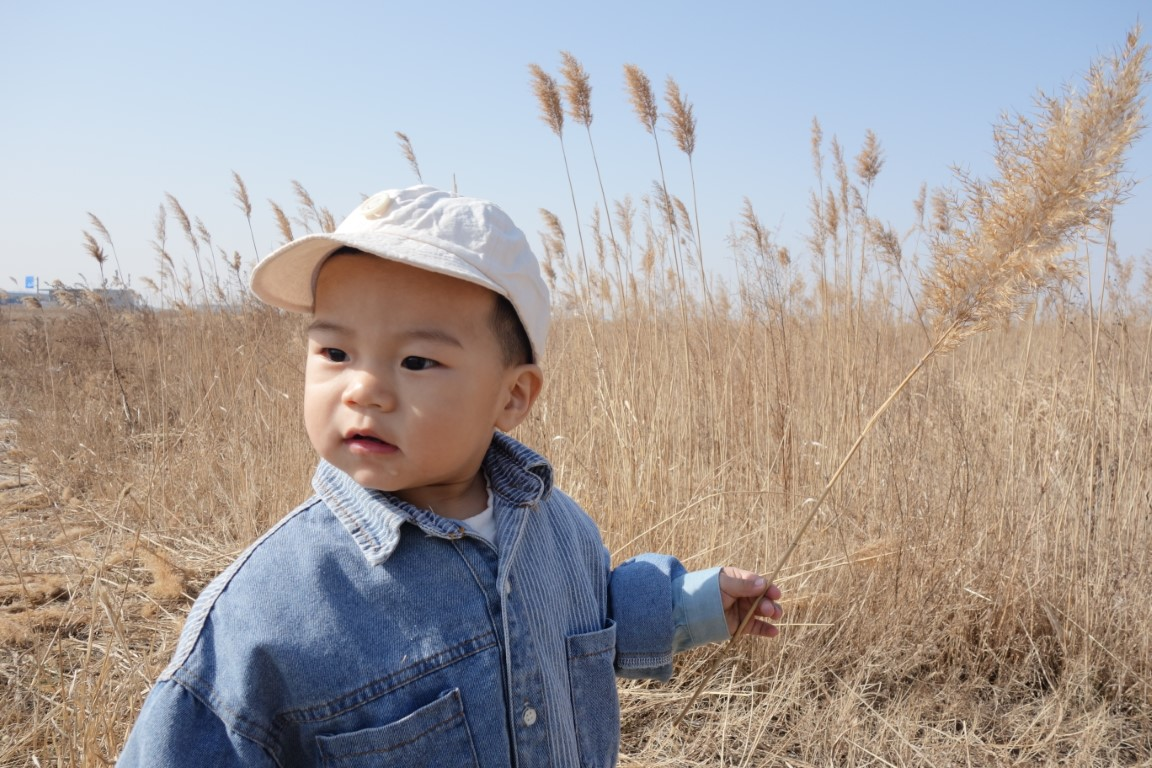
\includegraphics[height=.44\textwidth]{images/张沐凡}}
        \only<2>{
\includegraphics[height=.44\textwidth]{images/爱玛}}
        \only<3>{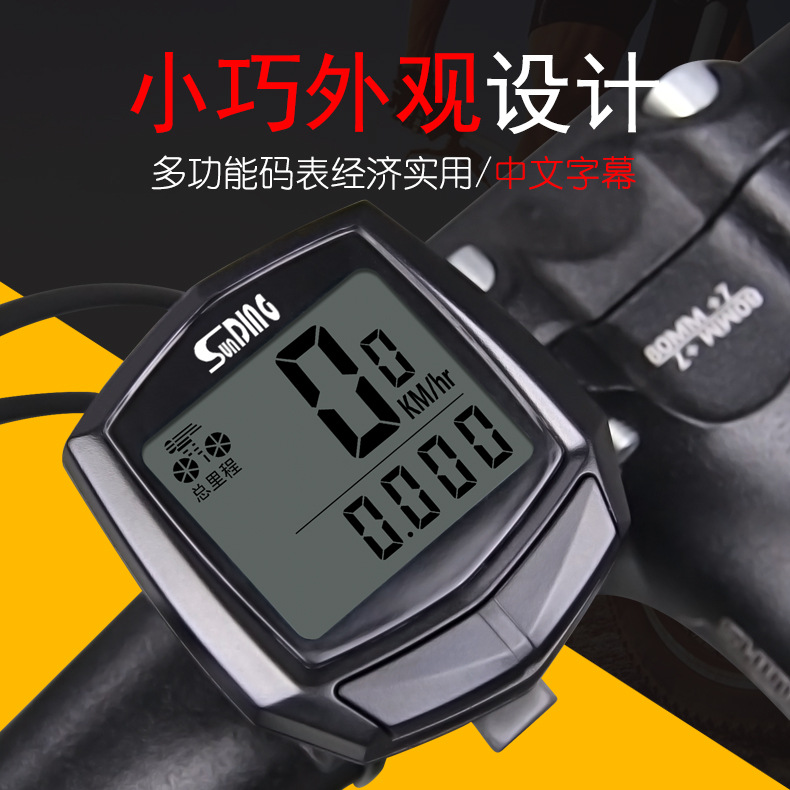
\includegraphics[height=.44\textwidth]{images/里程表.jpg} \quad 
        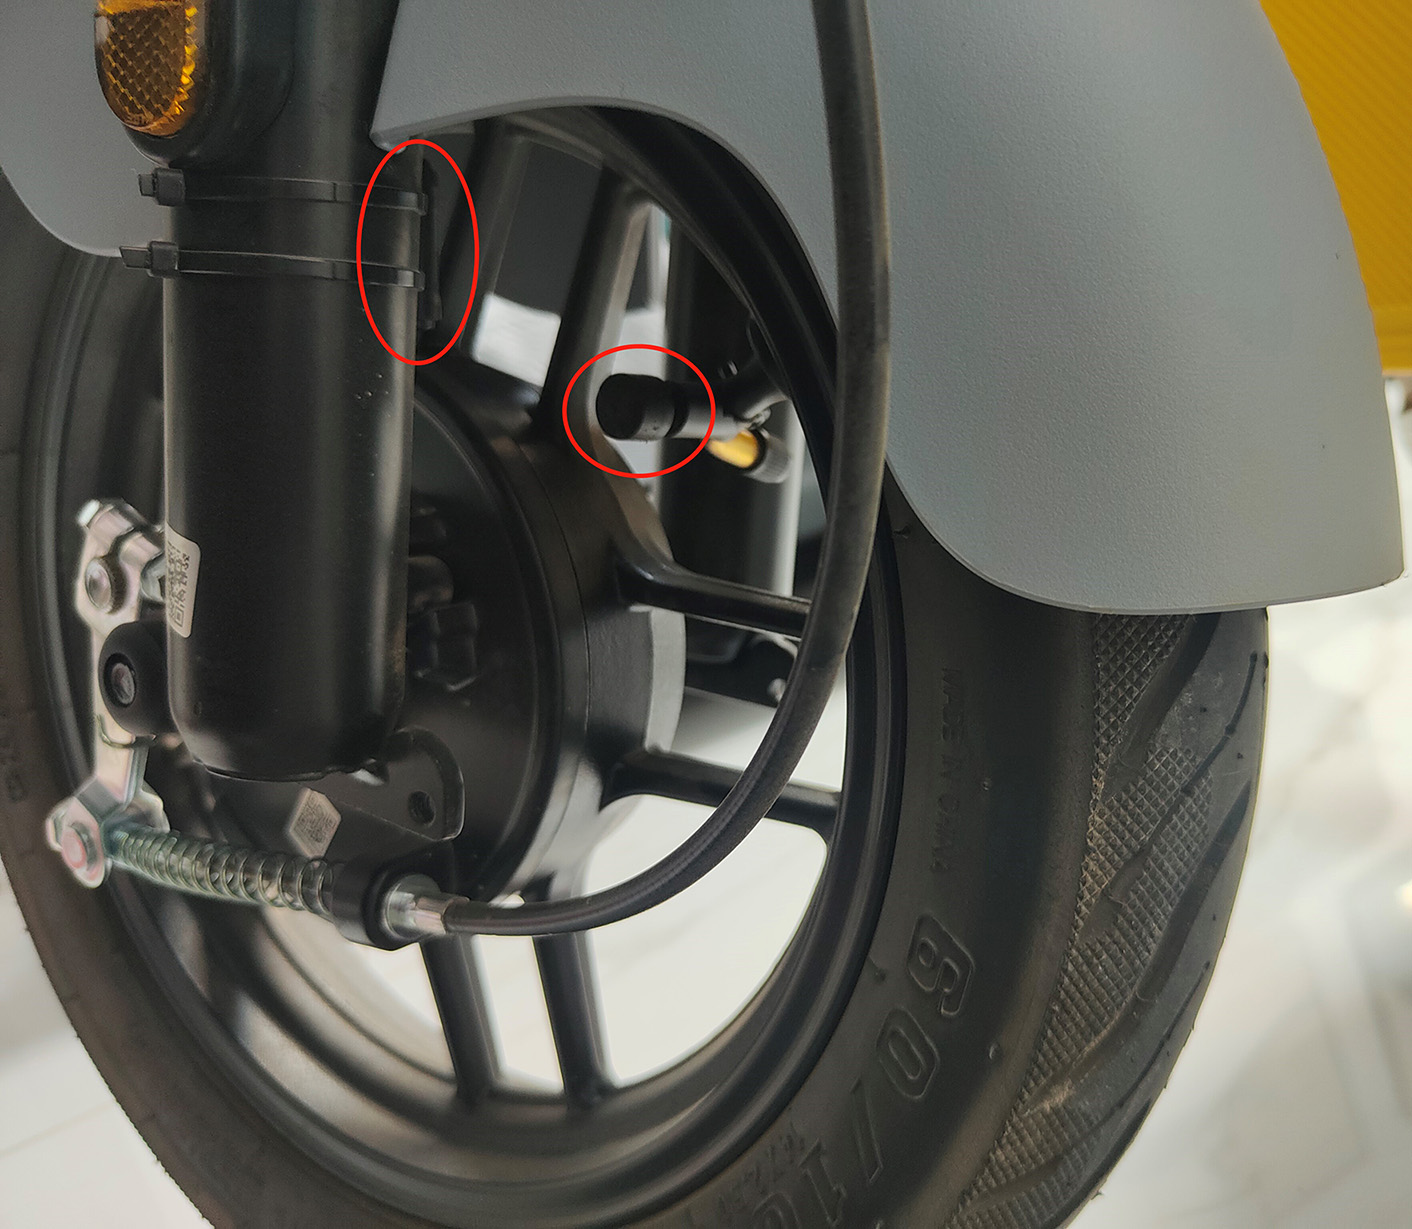
\includegraphics[height=.44\textwidth, width=.52\textwidth]{images/里程表原理3}}
    \end{figure}
\end{frame}

% \begin{frame}
%     \frametitle{磁传感器}
%     \begin{figure}[htpb]
%         \centering
%         
\includegraphics[height=.22\textwidth]{images/XBOX手柄}
%         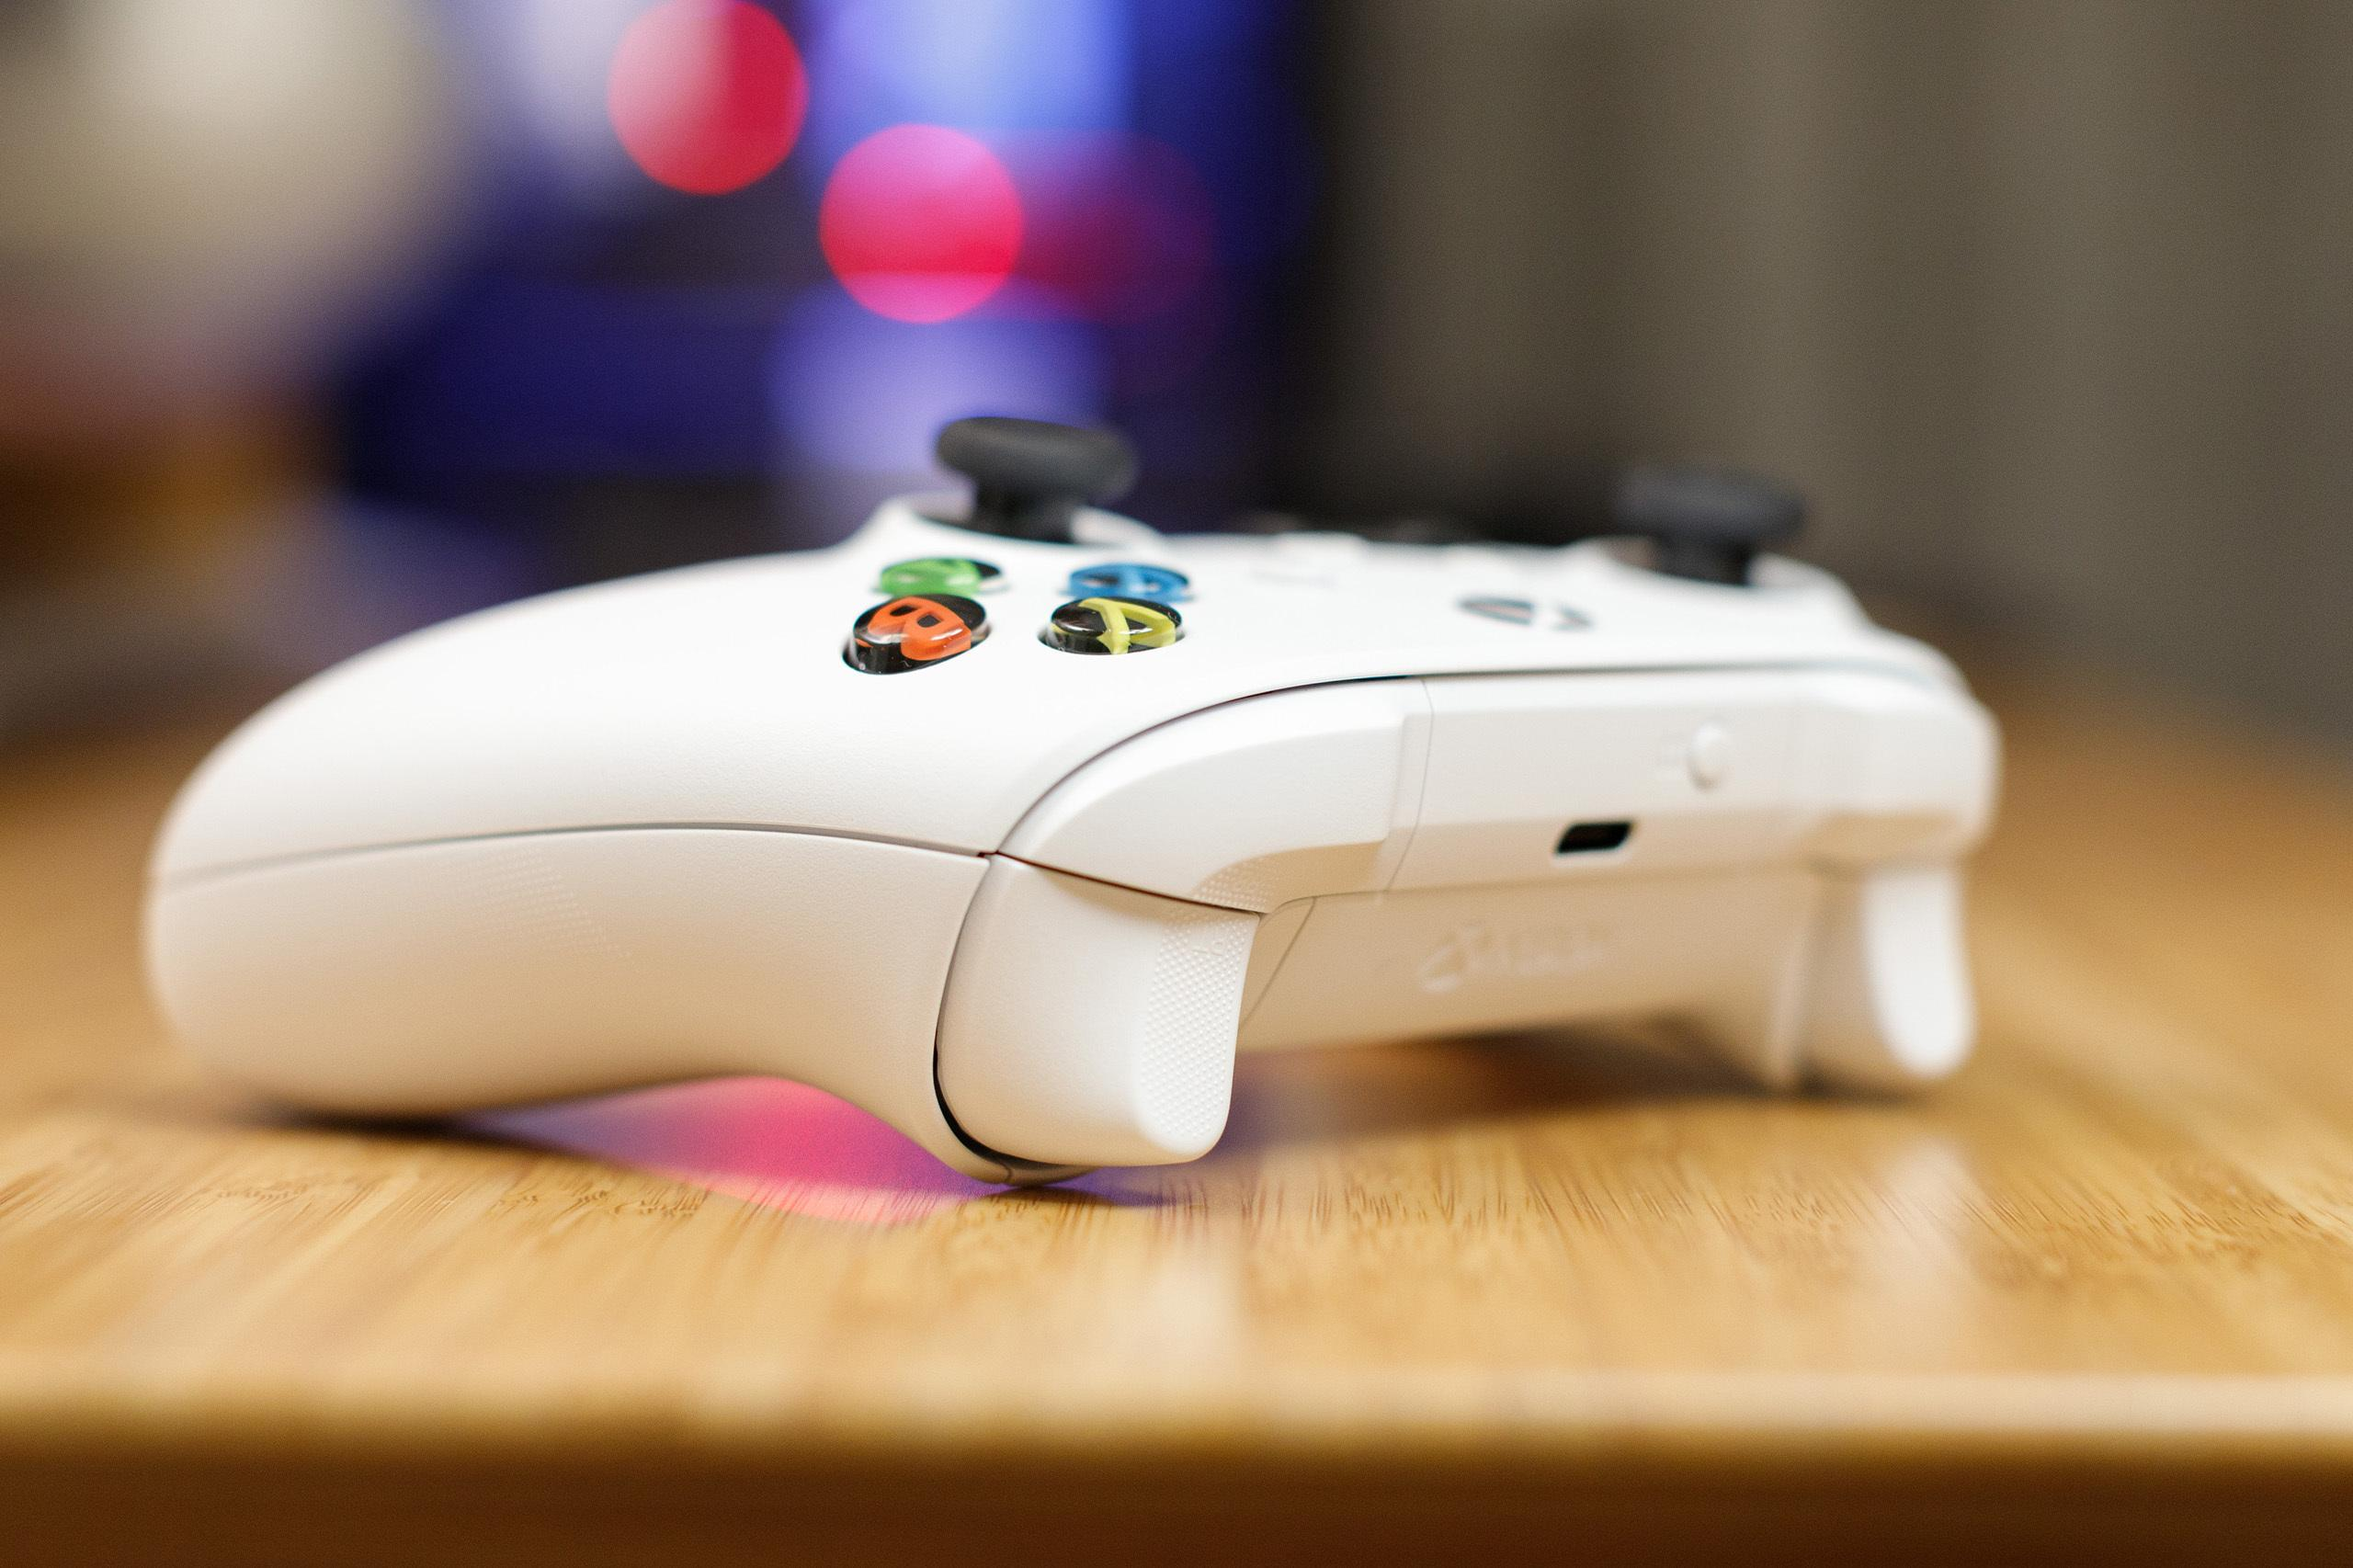
\includegraphics[height=.22\textwidth]{images/XBOX手柄扳机}
%         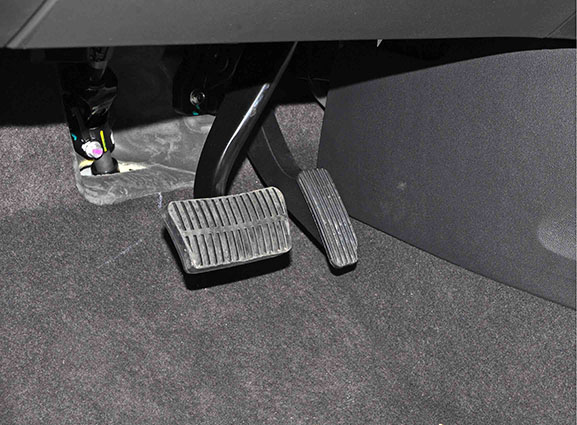
\includegraphics[height=.22\textwidth]{images/油门}
%         
\includegraphics[height=.22\textwidth]{images/GTR}
%         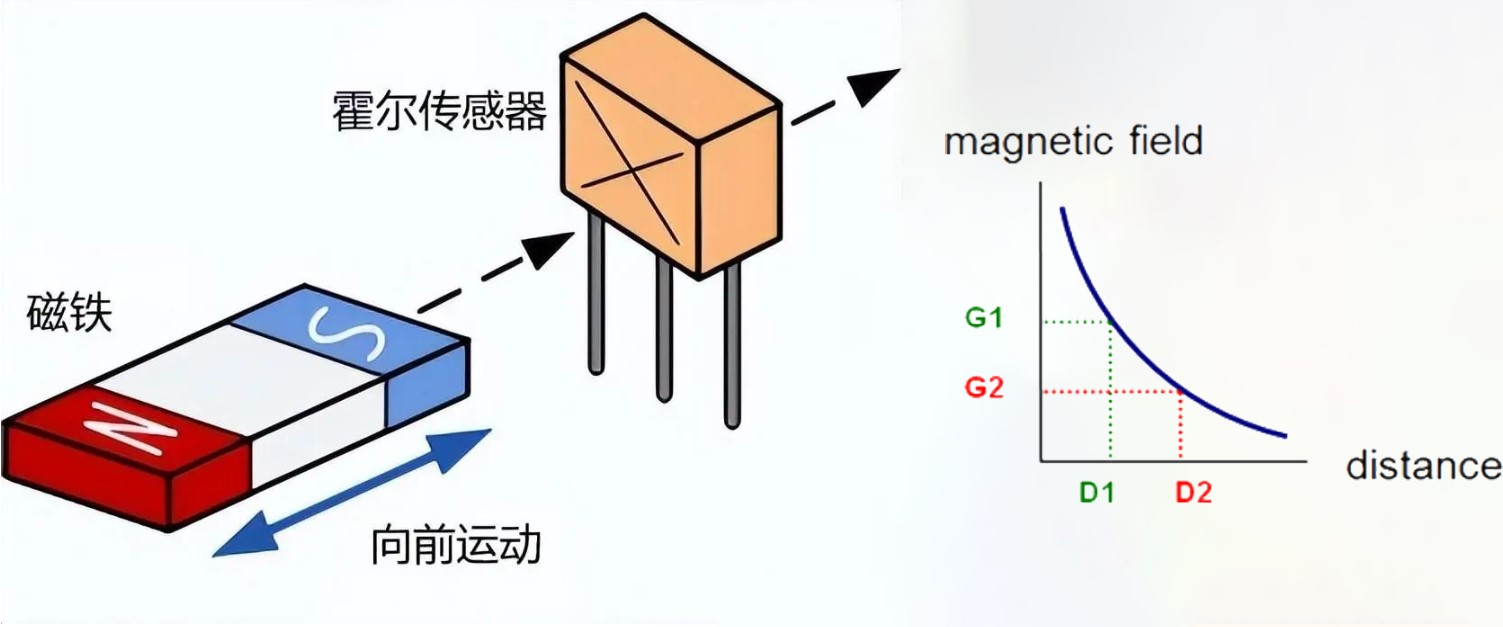
\includegraphics[height=.22\textwidth, width=.558\textwidth]{images/霍尔效应}
%     \end{figure}
% \end{frame}

% \begin{frame}
%     \frametitle{磁传感器}
%     \begin{figure}[htpb]
%         \centering
%         
\includegraphics[height=.223\textwidth]{images/Nintendo Switch.jpg} 
%         
\includegraphics[height=.223\textwidth]{images/漂移}
%         \pause
%         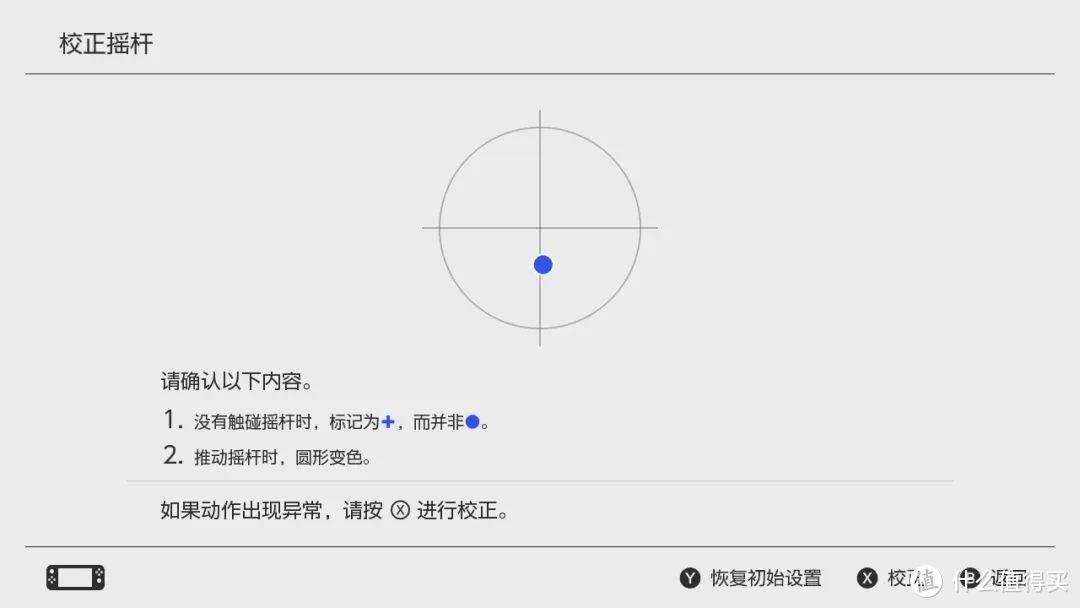
\includegraphics[height=.223\textwidth]{images/校正}
%         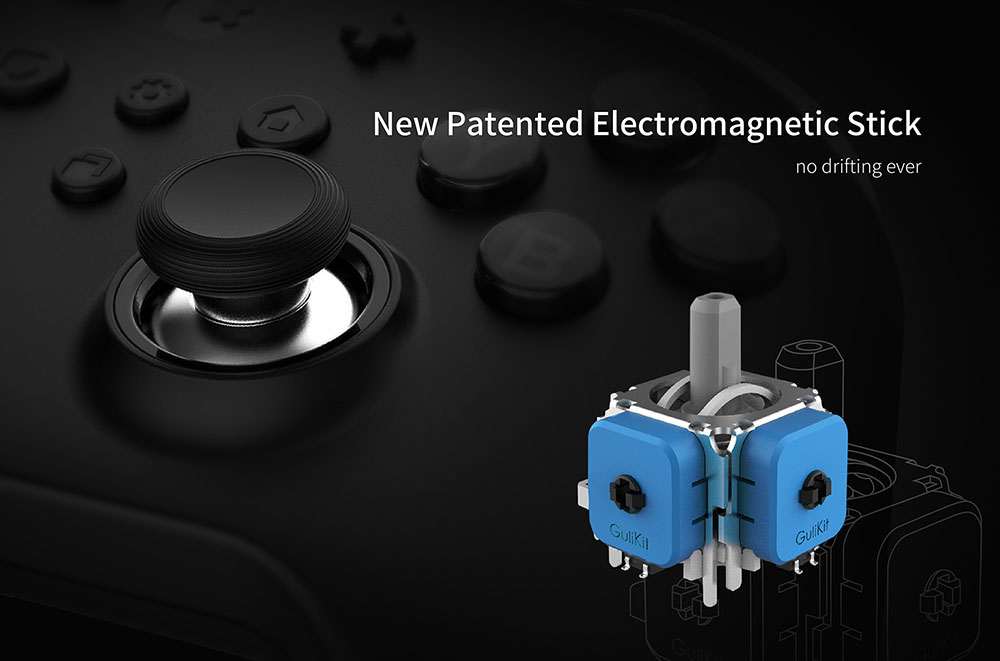
\includegraphics[height=.223\textwidth]{images/霍尔摇杆}
        
%     \end{figure}
% \end{frame}




\begin{frame}
    \frametitle{气体传感器}
    \begin{figure}[htpb]
        \centering
        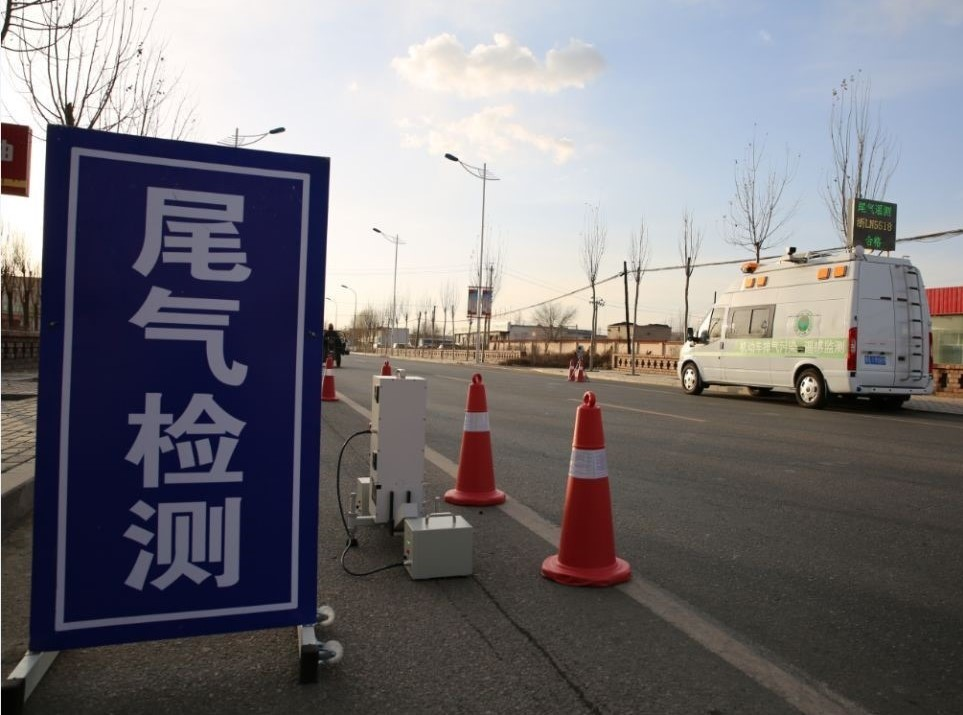
\includegraphics[height=.44\textwidth]{images/尾气监测}
    
\includegraphics[height=.44\textwidth]{images/查酒驾.jpg}
    \end{figure}
    
\end{frame}

% 机动车尾气遥感监测系统对道路行驶中车辆进行尾气监测，是最有效、最经济、最方便的监测方法，监测过程快速、高效，每辆遥感车一天可监测 5000 辆以上行驶中的车辆，既不影响司机正常行驶，也不会造成交通堵塞，监测效率是人工监测的10倍以上。

% 这台移动式遥感监测车带有一套特殊的尾气遥测仪，车上配备一台电脑主机，车顶架设一面LED屏。车辆后方一台监测主机和反射单元机，摆于车道的两侧，监测仪会发出紫外光和红外光，形成光的回路。当机动车通过时，尾气中所含的一氧化碳及氮氧化物会吸收红外光、紫外光，具体数值会通过主机的换算计算出尾气中一氧化碳及氮氧化物的浓度。仪器同时还配有高速摄像机，可以对在平行范围内通过的车辆进行牌照识别，最终可以将车辆的车牌号及尾气监测结果显示在仪器屏幕上。

\begin{frame}
    \frametitle{pH传感器}
    \begin{figure}[htpb]
        \centering
        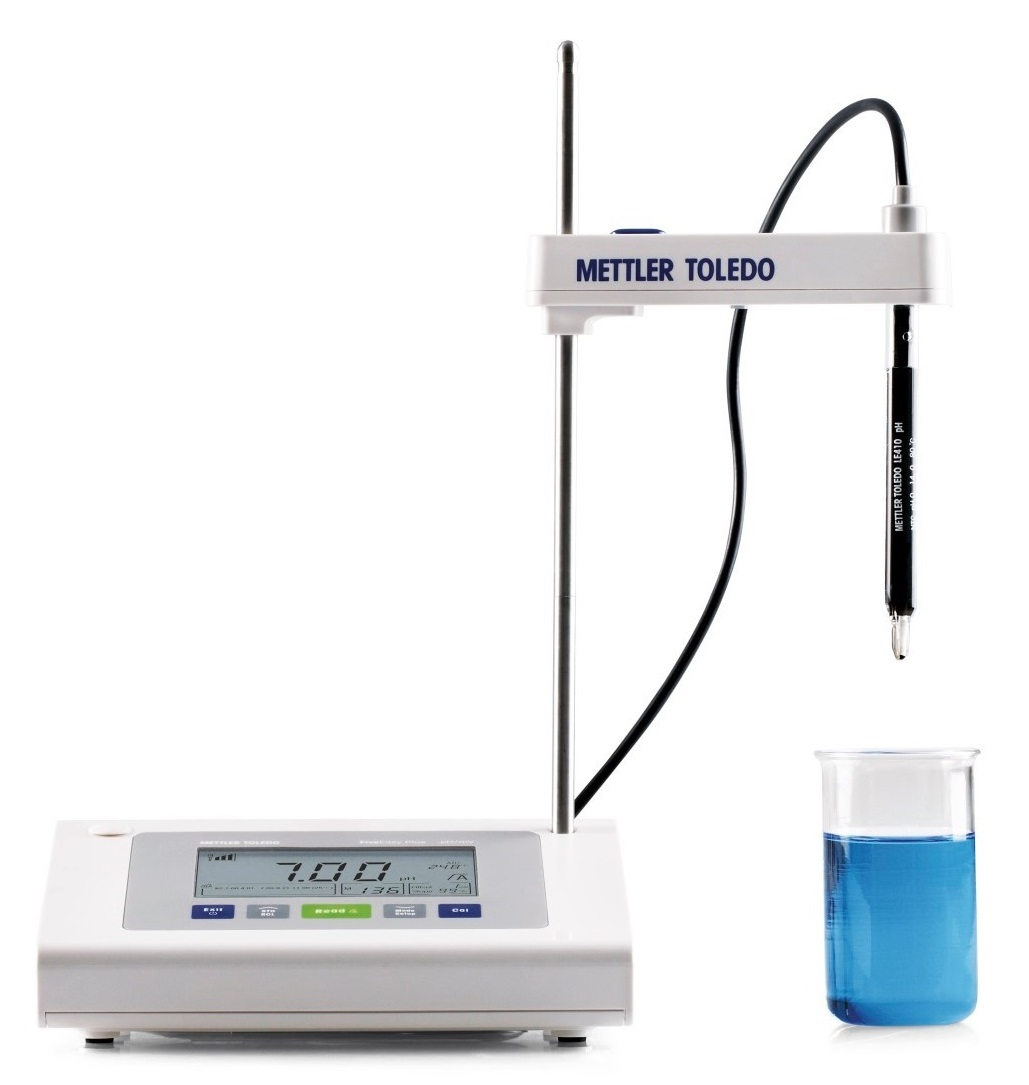
\includegraphics[height=.44\linewidth]{images/ph计.jpg} \qquad \qquad
        \includegraphics[height=.44\linewidth]{images/ph传感器}
    \end{figure}
\end{frame}
% 测量原理：
% pH传感器是由玻璃指示电极和参比电极组合在一起的复合电极。pH的测量是根据测量电极和参比电极组成的工作电池在溶液中测得的电位差，利用待测溶液的pH值与工作电池的电势大小之间的线性关系，来实现pH的在线监测。

\begin{frame}
    \frametitle{物位传感器}
    农业应用：农产品或农业生产资料的体积检测。
    \begin{figure}[htpb]
        \centering
        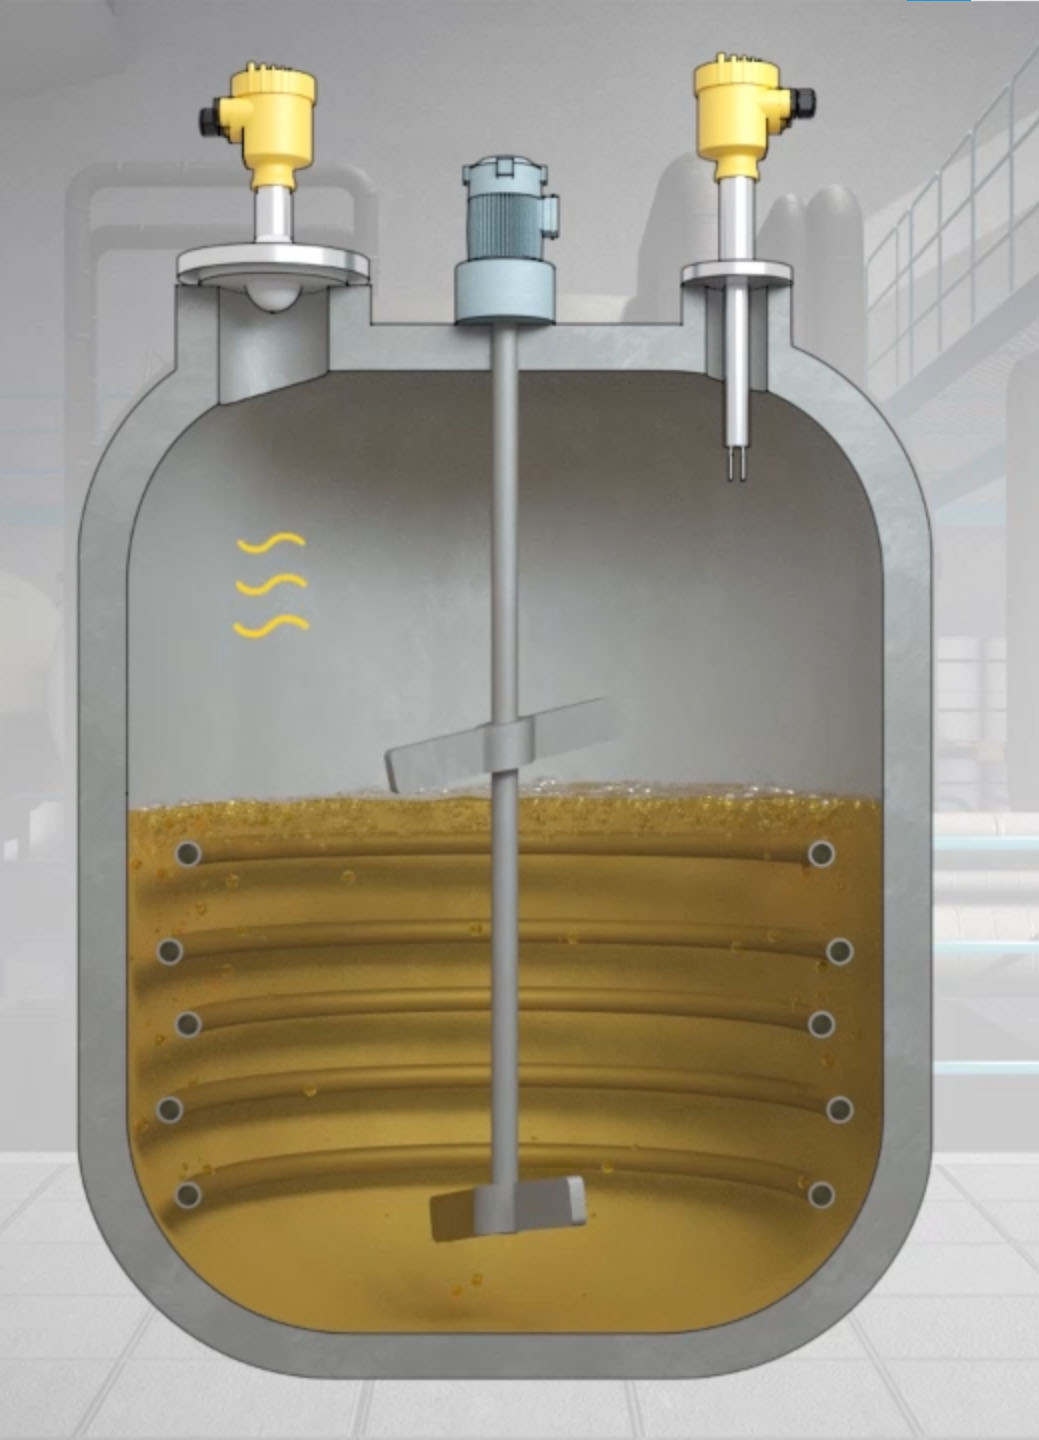
\includegraphics[height=.44\linewidth]{images/反应容器}
        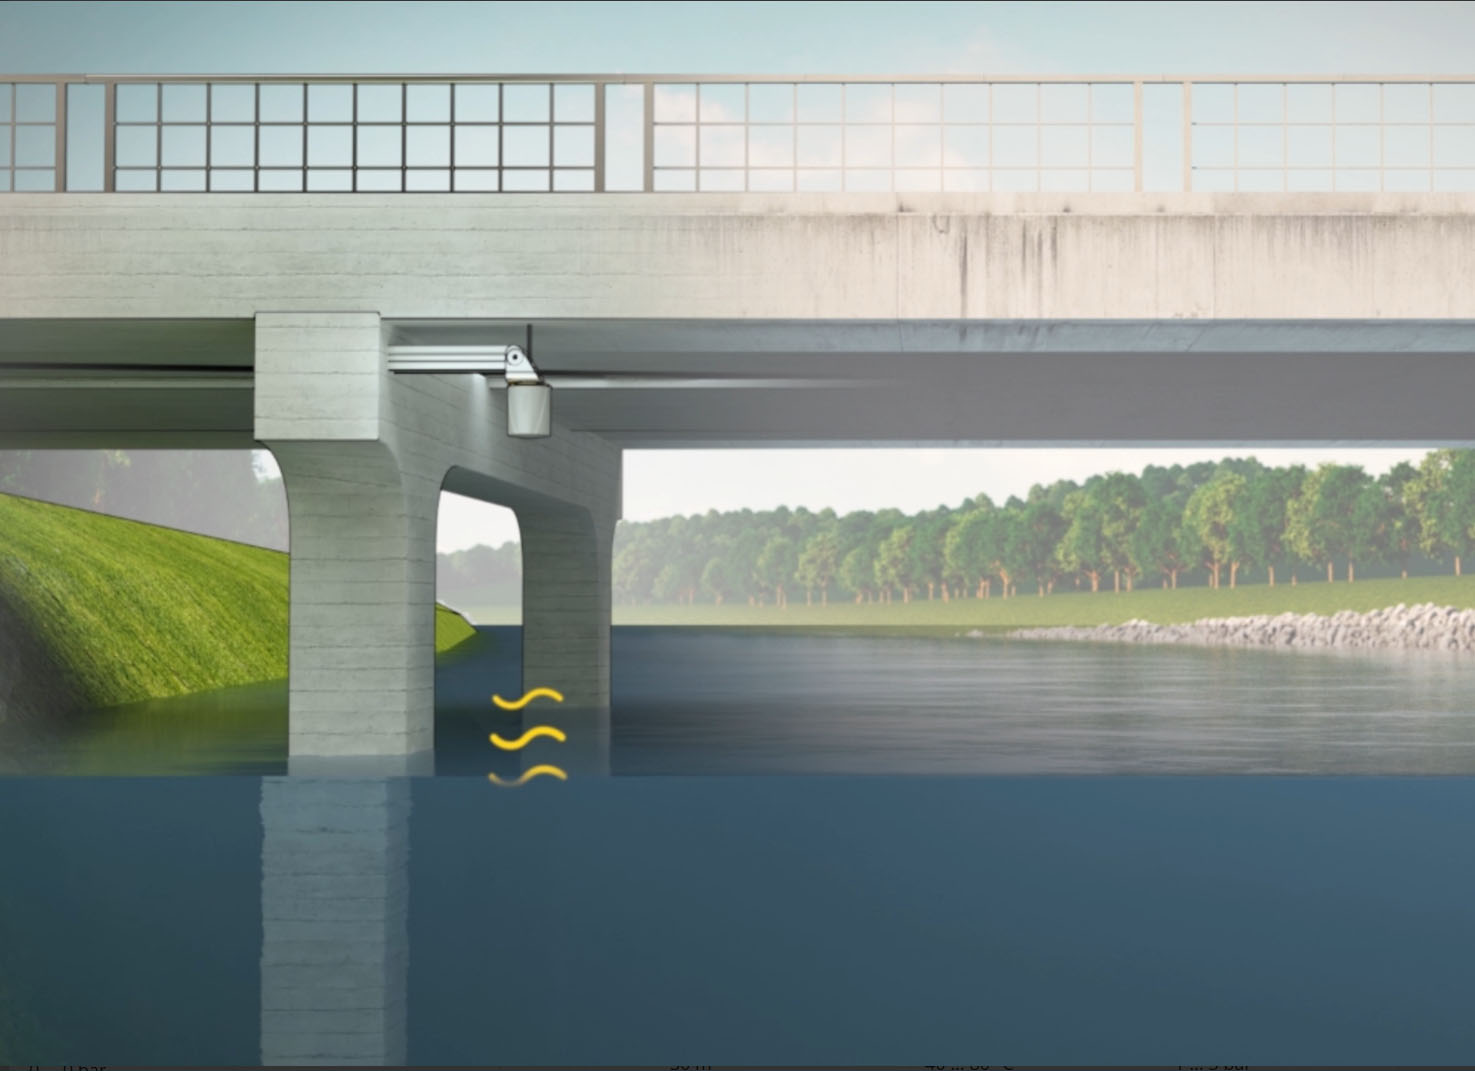
\includegraphics[height=.44\linewidth]{images/水位}
    \end{figure}
\end{frame}
% 采用无接触式超声波物位测量时，物位计朝介质的方向发出超声波脉冲，该介质又将这些脉冲反射回来。信号从发射到接收所需要的时间与容器中的物位成比例。对于简单的标准型应用，无论是在液体还是固料中，超声波物位计都是理想的测量仪表。 
% 在用雷达进行无接触式物位测量时，物位计从上方将微波信号发射给介质，该介质表面再将之反射。根据接收到的信号，物位计可测得与介质之间的距离，并由此计算出准确的物位。此测量方法既适用于液体，也适用于固料。
% 与脉冲式雷达物位计类似，超声波物位计也是利用回波的反射原理，来测量物位的高度，二者的唯一区别为雷达物位计采用的是电磁波，无需传播介质，但是超声波物位计采用的是机械波，其必须借助一定介质才能进行传播，所以当介质的压力、温度、密度、湿度等条件恒定时，超声波在介质中的传播速度是一个常数。


\begin{frame}
    \frametitle{流量/流速传感器}
    测量原理：超声波，卡罗曼涡流，转数 

    农业应用：灌溉农作物时监测灌溉量。
    \begin{figure}[htpb]
        \centering
        \setcounter{subfigure}{0}
        \subfloat[电磁式流量传感器]{
\includegraphics[height=4cm]{电磁式流量传感器}}\quad
        \subfloat[涡流流量传感器]{
\includegraphics[height=4cm]{涡流流量传感器}}\quad
        \subfloat[容积式流量传感器]{
\includegraphics[height=4cm]{容积式流量传感器}}
    \end{figure}
\end{frame}


\begin{frame}
    \frametitle{振动/冲击/加速度传感器}
    测量原理：阻抗变化，静电效应，MEMS

    农业应用：农业机械运行状态检测，例如振动，加速度，角速度等
    \begin{figure}[htpb]
        \centering
        \setcounter{subfigure}{0}
        \subfloat[冲击传感器]{
\includegraphics[height=4cm]{冲击传感器}}\quad
        \subfloat[振动传感器]{
\includegraphics[height=4cm]{振动传感器}}\quad
        \subfloat[加速度传感器]{
\includegraphics[height=4cm]{加速度传感器}}
    \end{figure}
\end{frame}


\begin{frame}
    \frametitle{生物传感器}
    测量原理：酶传感器，微生物传感器，DNA传感器，细胞传感器

    农业应用：农药残留量分析、微生物和毒素的检验、食品鲜度的检测、水环境监测等

    \begin{figure}[htpb]
        \centering
        \setcounter{subfigure}{0}
        \subfloat[农药残留检测]{
\includegraphics[height=4cm]{农药残留检测}}\quad
        \subfloat[食品检测]{
\includegraphics[height=4cm]{食品检测}}\quad
        \subfloat[水质监测]{
\includegraphics[height=4cm]{水质监测}}
    \end{figure}
\end{frame}


\begin{frame}
    \frametitle{智能手表/手环中的传感器}
        \begin{minipage}{0.3\linewidth}
            \begin{figure}[htpb]
                \centering
                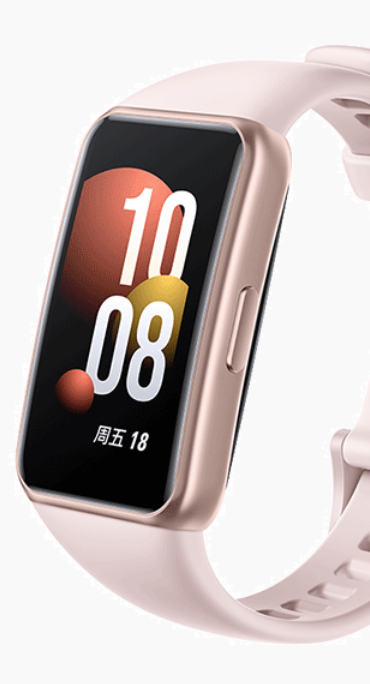
\includegraphics[height= 200pt]{images/手环7}
            \end{figure}
        \end{minipage}\hfill
        \begin{minipage}{0.68\linewidth}
            
            $\vcenter{\hbox{
\includegraphics[height= 25pt]{images/抬腕亮屏}}}$ {\bfseries 抬腕亮屏} \qquad 加速度传感器、陀螺仪

            \bigskip
            $\vcenter{\hbox{
\includegraphics[height= 25pt]{images/记步}}}$ {\bfseries 记步} \qquad \qquad 加速度传感器

            \bigskip
            $\vcenter{\hbox{
\includegraphics[height= 25pt]{images/心率}}}$ {\bfseries 心率} \qquad \qquad 光学心率传感器、生物电阻抗传感器

            \bigskip
            $\vcenter{\hbox{
\includegraphics[height= 25pt]{images/血氧}}}$ {\bfseries 血氧} \qquad \qquad 光学传感器

            \bigskip
            $\vcenter{\hbox{
\includegraphics[height= 25pt]{images/睡眠}}}$ {\bfseries 睡眠监测} \qquad 加速度传感器、心率传感器
        \end{minipage}
    
\end{frame}

% 抬腕亮屏：通过加速度传感器和陀螺仪检测手环状态，还会涉及一些复杂的算法，因为抬腕亮屏不仅要判断手环的位置、表盘朝向变化，还要综合考虑其他因素，保证检测到的是真的“抬腕”，从而避免不必要的亮屏耗电。
% 记步：重力加速度传感器。通过获取三个方向的加速度来获取加速度数据。对于加速度数据进行分析，判断是否为正常行走类型（包括前进，后退，上楼，下楼，跑步等类型）。通过以上数据，计算出当前使用者的步长，最终统计出行走时间，距离，运动强度等数据。
% 心率：最常见的是光学心率传感器，原理是通过LED绿光照射紧贴传感器的皮肤和附近血管，通过测算光线被吸收的波动来判断心率状态，辅助运动检测，也可以检测心脏异常，及时反馈报警。血液之所以呈现红色，是因为它反射红光并吸收绿光。心脏跳动时，流经手腕的血流量会增加，吸收的绿光也会增加；在心跳间隔期间减少。
% 心率2：另一种电极式心率传感器。电极可以在与“心率”App 或移动心电图房颤提示软件搭配使用时测量通过你心脏的电信号，经过峰值检测可以获得心率。当你将手指放在数码表冠上时，就会在你的心脏和双臂之间形成一个闭合电路，从而捕捉到通过你胸部的电脉冲。https://support.apple.com/zh-cn/HT204666
% 血氧:光学传感器。原理与心率检测一致，都是通过背面贴近皮肤的模块发射光线，利用光敏电阻检测被血液吸收一部分的光线波动来分析血氧状态，不同的是这个过程发出的光线往往是红外光，而且容易受到各种因素干扰，因此手环/手表上的血氧检测准确度有限，只能作为参考。​
% 睡眠监测：主要靠心率传感器、加速度传感器来实现。简单来说，人在清醒状态和睡眠状态的心率有很大的差别，加速度传感器能有效监测人的位移变量，就是监测你的动作，人在入睡的时候，手肯定不会有较大的垂直高度位移。当我们处于睡眠状态的时候，心率一般情况下会下降；而当用户睡得很深的时候，心率会下降的更低。而手环通过监测我们的一个心率变异性，从而来判断我们的睡眠时间和睡眠的深浅。

\section{农业生产全过程数字化技术}

\begin{frame}
    \frametitle{农业数据采集}
    我国农业生产存在人工成本迅速增加；生产规模小；方式落后；效率效益低等问题。发展智慧农业，通过电脑替代人脑，机器替代人力可以很好的解决这些问题。首先需要建设人机协同的天空地一体化数据信息采集体系，获取农业数字化信息。

    采集方法：
    \begin{figure}[htpb]
        \centering
        \setcounter{subfigure}{0}
        \subfloat[温湿度传感器]{
\includegraphics[height=3cm]{温湿度传感器}}\hfill
        \subfloat[光照传感器]{
\includegraphics[height=3cm]{光照传感器}}\hfill
        \subfloat[土壤温湿度传感器]{
\includegraphics[height=3cm]{土壤温湿度传感器}}\hfill
        \subfloat[CO$_2$浓度传感器]{
\includegraphics[height=3cm]{CO2浓度传感器}}
    \end{figure}
    
    

\end{frame}


\subsection{3S技术}

\begin{frame}
    \frametitle{3S技术}
    3S技术是全球卫星导航系统(Global Navigation Satellite System，GNSS)、遥感技术(Remote sensing，RS)和地理信息系统(Geography information systems，GIS)的统称，是空间技术、传感器技术、卫星定位与导航技术和计算机技术、通讯技术相结合，多学科高度集成的对空间信息进行采集、处理、管理、分析、表达、传播和应用的现代信息技术 。

    \bigskip
    在农业领域，“3S”技术可以为现代农业建立与之相适应的地理信息系统，为农业的规划、设计、管理、生产、决策过程提供更为精确的信息，在农业领域应用优势非常明显。上世纪80年代起，“3S”技术在我国农业领域开始有所应用，历经多年发展，产生了巨大的经济和社会效益，成为推动“数字农业”发展的重要手段。

\end{frame}

\begin{frame}
    \frametitle{全球卫星导航系统 GNSS}
    \begin{figure}[htpb]
        \centering
        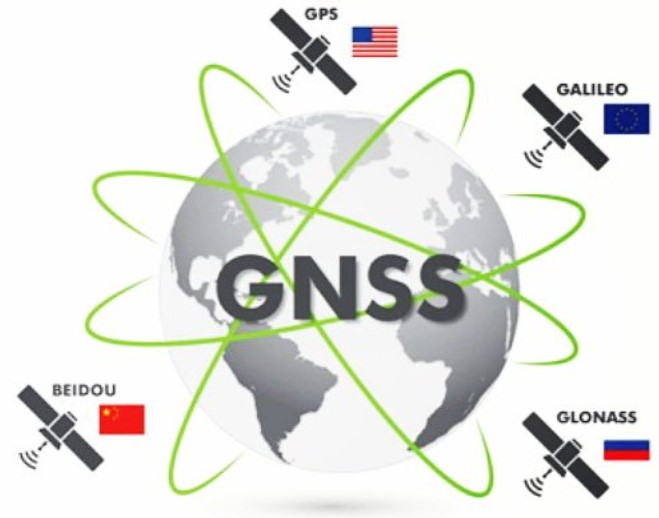
\includegraphics[height=.4\linewidth]{images/GNSS}
        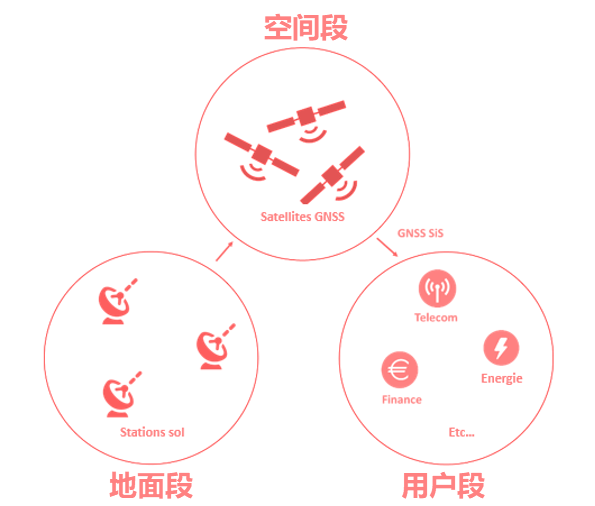
\includegraphics[height=.4\linewidth]{images/GNSS组成}
    \end{figure}
\end{frame}


\begin{frame}
    \frametitle{智能手机---卫星导航大规模在社会个人普及}
    \begin{figure}[htpb]
        \centering
        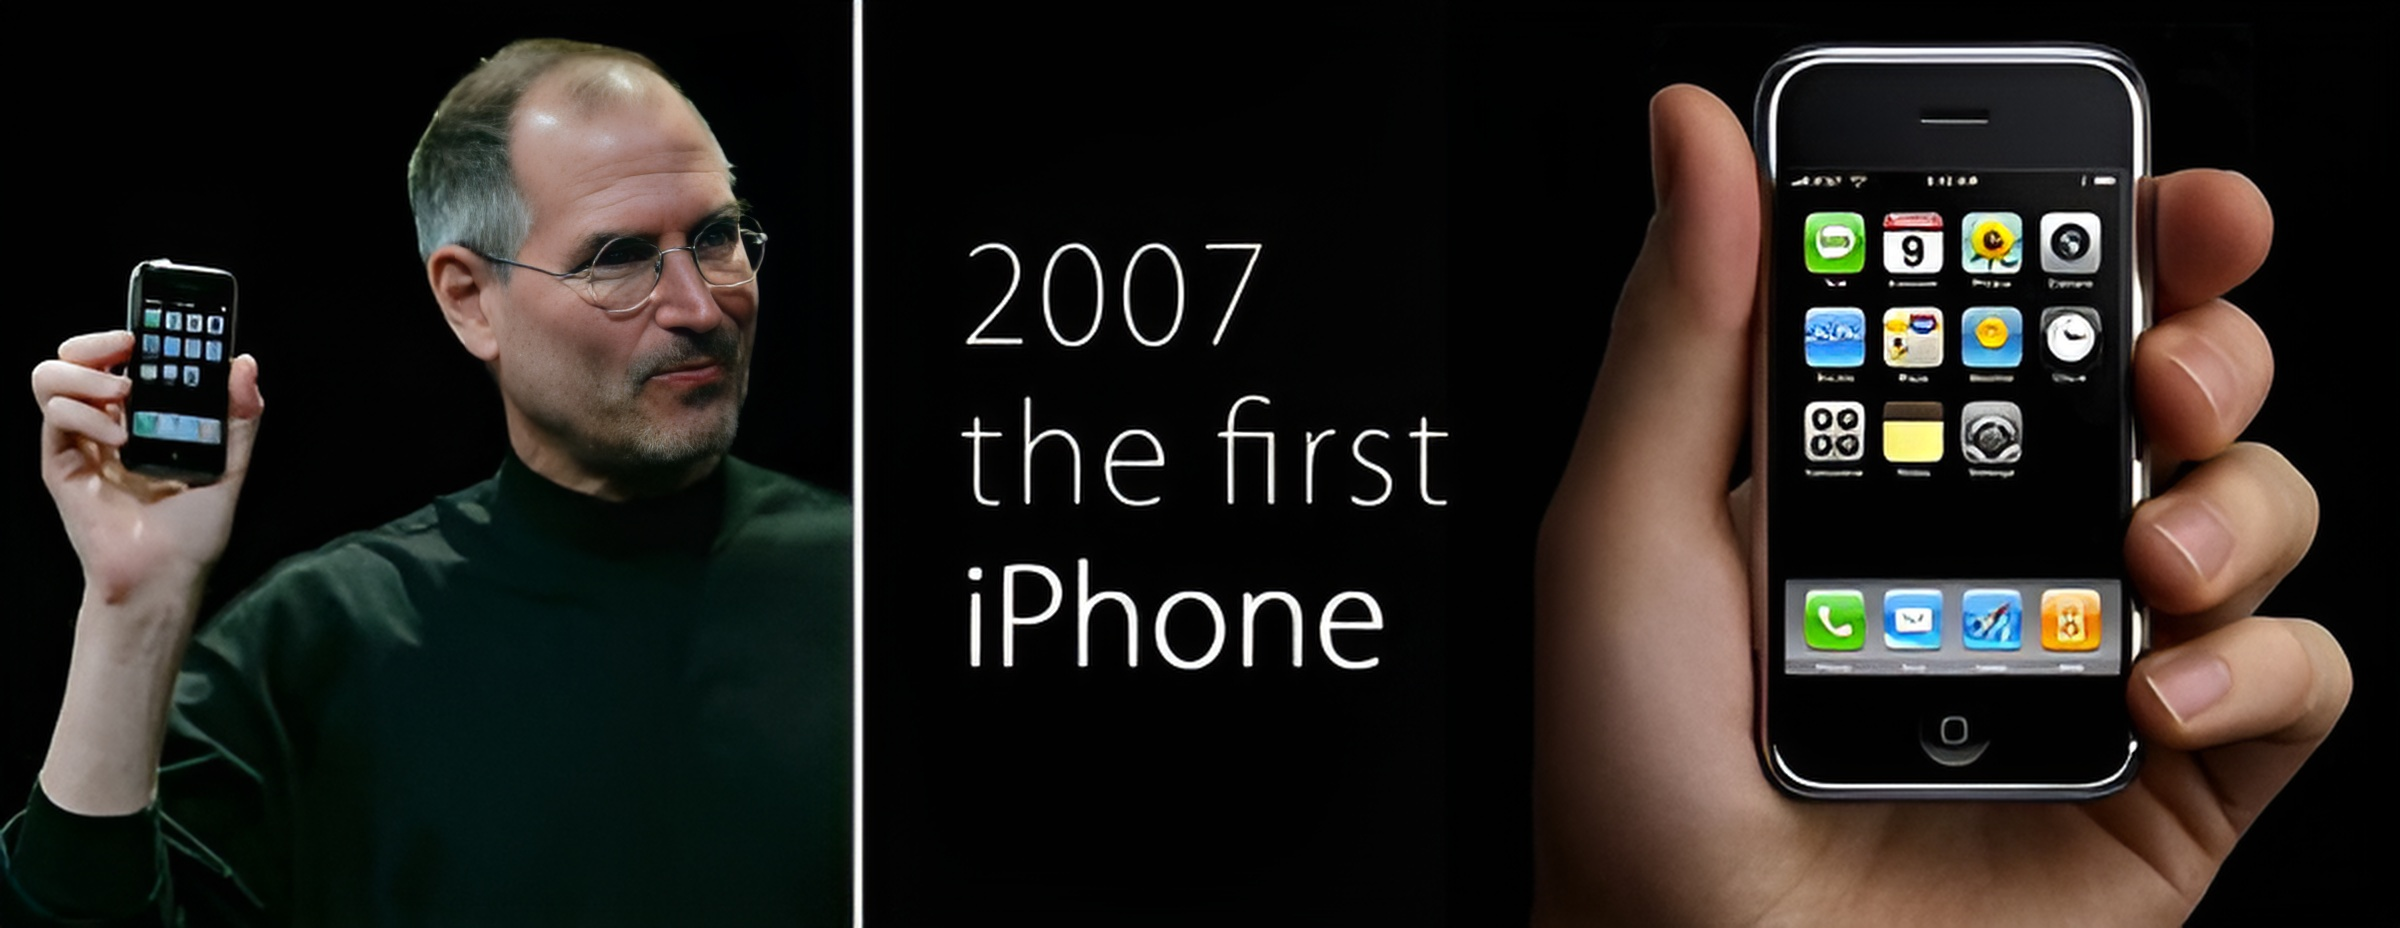
\includegraphics[width=\linewidth]{images/iphone}
    \end{figure}
\end{frame}

\begin{frame}
    \frametitle{我到哪了？}
        \begin{minipage}{0.43\linewidth}
            \begin{figure}[htpb]
                \centering
                {\bfseries 二十年前：地图}

                ~~~

                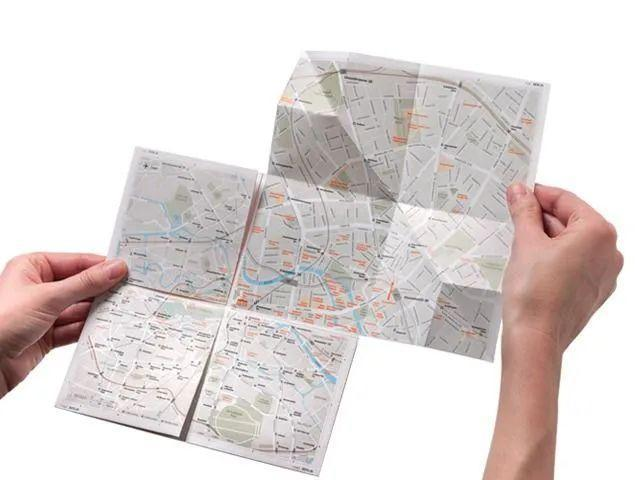
\includegraphics[height=120pt]{images/纸质地图}
            \end{figure}
        \end{minipage}\hfill
        \begin{minipage}{0.55\linewidth}
            \begin{figure}[htpb]
                \centering
                {\bfseries 现在：导航}

                ~~~

                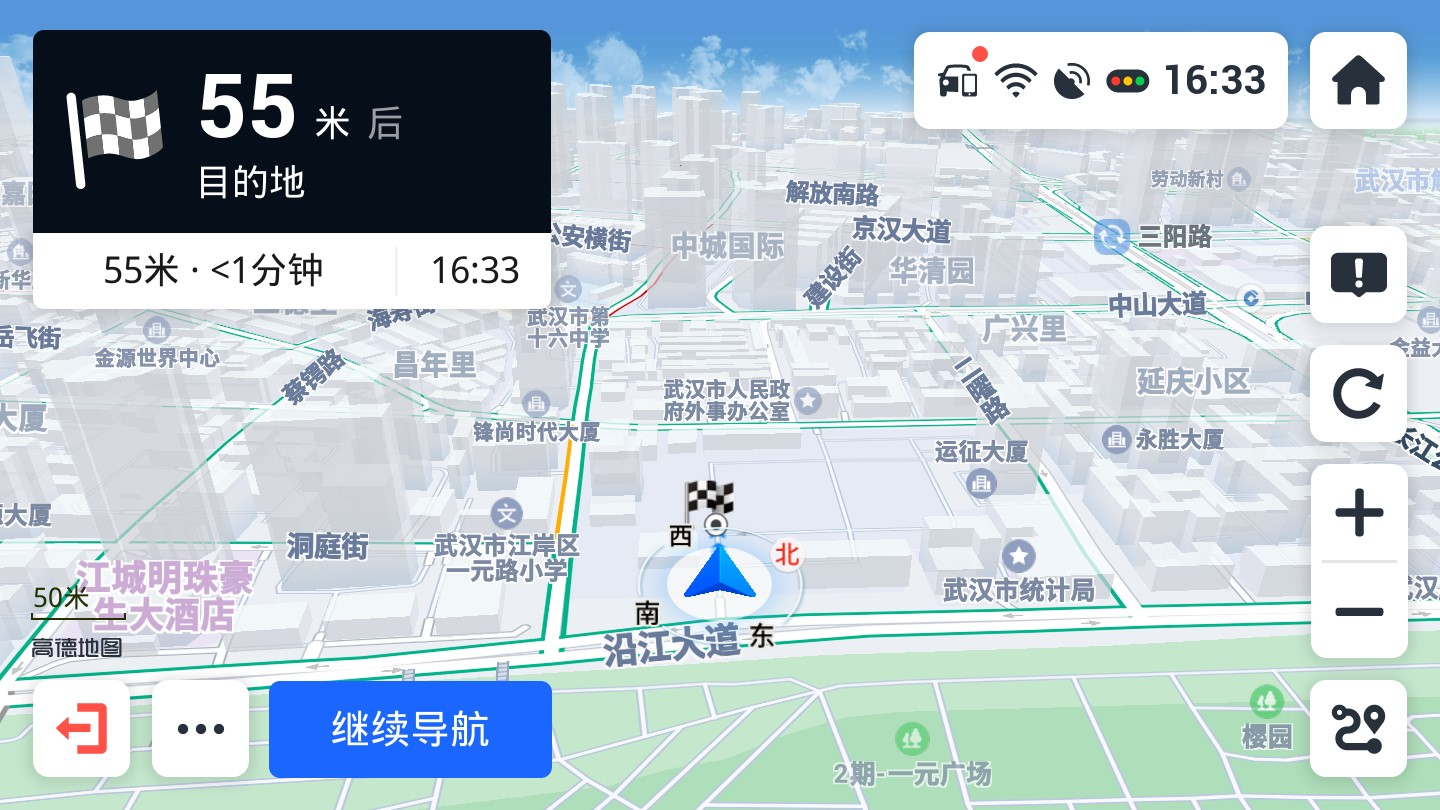
\includegraphics[height=120pt]{images/车载导航}
            \end{figure}
        \end{minipage}
\end{frame}


\begin{frame}
    \frametitle{“你在哪里？”}
        \begin{minipage}{0.48\linewidth}
            \begin{figure}[htpb]
                \centering
                {\bfseries 二十年前：“我在村口的大树下”}
                \bigskip

                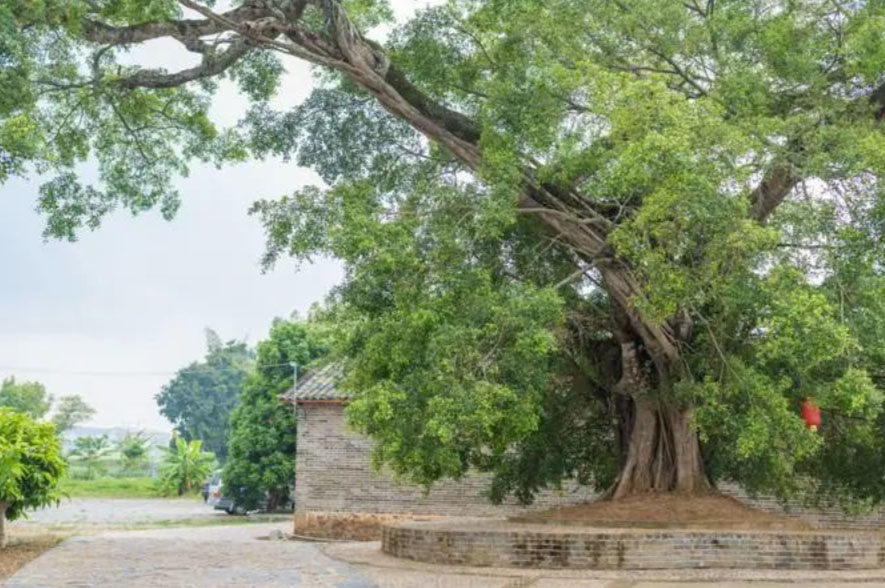
\includegraphics[height=115pt]{images/大树}
            \end{figure}
        \end{minipage}\hfill
        \begin{minipage}{0.5\linewidth}
            \begin{figure}[htpb]
                \centering
                {\bfseries 现在：卫星定位}
                \bigskip

                
\includegraphics[height=115pt]{images/位置}
            \end{figure}
        \end{minipage}
\end{frame}



\begin{frame}
    \frametitle{海湾战争---卫星导航系统第一次大规模的使用}
    伊方拥有百万雄师，5800多辆坦克，4600多辆装甲车和步兵战车，3万门火炮，不少全球军事学家一开始都预测会打成僵持战。

    然而，只有30万军队的美国联军，仅仅用了42天，便以美军146人阵亡、467人受伤，伊军则伤亡超10万人的代价，把伊拉克的百万雄师彻底打垮。这场战争一反传统作战方式，美国对伊拉克祭出了大量精确制导武器，288枚“战斧”命中率更是高达98\% ，对伊的打击如同无头苍蝇般吊打。

    这场战争，是一场非对称战争。美军对伊拉克的打击，可以说是降维打击。因为伊拉克，还停留在机械化战争的时代。而美国，已经进入信息化战争的时代。这两种战争时代的差别，就在于有没有卫星导航系统（GPS）。

\end{frame}
\begin{frame}
    \frametitle{银河号事件}
    1993年7月23日，美国以获得情报为由，指控中国“银河号”货轮向伊朗运输制造化学武器的原料，并威胁要对中国进行制裁。美国一度直接掐断了银河号的GPS信号，让其在公海航行中失去行动力。最终，银河号只能成为砧板上的鱼肉，任人宰割。

    1993年9月4日，“银河号”货轮上最后一个货箱被检查完毕，没有发现任何化学武器，“银河号”被迫中止正常航运长达33天。

    这一事件深深地警醒了中国，如果没有自主的全球导航系统，"银河号"事件绝不会是最后一次。

    1994年12月，北斗导航实验卫星系统工程获得国家批准。
\end{frame}

\begin{frame}
    \frametitle{北斗卫星导航系统 \link{http://www.beidou.gov.cn/}}
    北斗卫星导航系统（以下简称北斗系统）是中国着眼于国家安全和经济社会发展需要，自主建设运行的全球卫星导航系统，是为全球用户提供全天候、全天时、高精度的定位、导航和授时服务的国家重要时空基础设施。 
    \bigskip

    “三步走”发展历程：
        \begin{itemize}
          \item 2000年年底，建成北斗一号系统，向中国提供服务；
          \item 2012年年底，建成北斗二号系统，向亚太地区提供服务；
          \item 2020年，建成北斗三号系统，向全球提供服务。 
        \end{itemize}
\end{frame}

\begin{frame}
    \frametitle{新时代北斗精神}
    \begin{center}        
        {\huge \cbf{自主创新、开放融合、万众一心、追求卓越}} % 新时代北斗精神
    \end{center}    
\end{frame}

\begin{frame}
    \frametitle{北斗 VS GPS}
\begin{table}[]
    \begin{tabular}{@{}lll@{}}
    \toprule
    \multicolumn{1}{c}{} & \multicolumn{1}{c}{北斗} & \multicolumn{1}{c}{GPS} \\ \midrule
    卫星覆盖                 & 55颗                    & 31颗                     \\
    通讯信号                 & 三频信号                   & 双频信号                    \\
    短报文通信                & 北斗独创                   & 无                       \\
    分步开通                 & 支持局部卫星组网               & 必须全部卫星                  \\
    民用定位精度 \qquad              & 10米，亚太地区5m    \qquad         & 10米                     \\
    军用定位准度               & 0.5米                   & 0.3米                    \\ \bottomrule
    \end{tabular}
    \end{table}
\end{frame}


\begin{frame}
    \frametitle{华为Mate50，短报文通信\link{http://www.beidou.gov.cn/yw/xwzx/202209/t20220929_24645.html}}
    \begin{figure}[htpb]
        \centering
        \setcounter{subfigure}{0}
        \subfloat{
\includegraphics[height=6cm]{mate50}}\hfill
        \subfloat{
\includegraphics[height=6cm]{mate50-2}}
    \end{figure}
\end{frame}


\begin{frame}
    \frametitle{华为Mate60，卫星电话}
    \begin{figure}[htpb]
        \centering
        
\includegraphics[width=.8\linewidth]{mate60}
    \end{figure}
\end{frame}


\begin{frame}
    \frametitle{天通一号卫星移动通信系统\link{http://www.tdstar.cn/industry/157.html}}

    \begin{itemize}
      \item 01星2016年发射，中国地区无缝覆盖（领土/领海/第一岛链）
      \item 02/03星覆盖亚洲17个国家：日本、韩国、菲律宾、帕劳、越南、老挝、柬埔寨、泰国、马来西亚、新加坡、印尼、文莱、东帝汶、缅甸、孟加拉国、不丹、尼泊尔
    \end{itemize}
    \begin{figure}[htpb]
        \centering
        
\includegraphics[width=.7\linewidth]{天通}
    \end{figure}
\end{frame}


% 北斗的未来，是大众规模化应用。因为卫星导航系统非常烧钱，无论是早期的研发，发射卫星，还是后期的维护运营，都非常烧钱。卫星也是有使用寿命的，报废了就得再发射一颗上去。所以北斗也要恰饭，要挣钱养活自己才行。美国的GPS是怎么挣钱养活自己的呢？它是通过卖GPS定位芯片，来挣钱的。咱们每个人手机里，都有美国GPS的定位芯片，每一个芯片，都需要向美国人交授权费才能用。2017年以后，随着国产手机的强势崛起，华为、小米、OPPO等品牌在世界手机行业站稳脚跟，北斗也找到了自己的用武之地。这两三年你买的国产手机里，都安装有北斗系统，都有北斗芯片，你已经用真金白银，为北斗助力了。

% 北斗系统未来在全球应用市场的基本格局：

% 第一，北斗在全球最大的应用市场，肯定是在中国。

% 虽然目前美国GPS占据了中国很大的民用市场，但未来北斗系统肯定会逐渐取而代之，美国GPS在中国将逐渐变成北斗的辅助系统，而非主流的卫星导航系统。

% 第二，北斗在全球最难抢占的市场，肯定是美国、欧洲、俄罗斯、印度、日本这些拥有自主卫星导航系统的国家，甚至很难抢占加拿大、澳大利亚等亲美国家的主流市场。

% 很难抢占主流市场，并不意味着无法进入，毕竟北斗系统拥有一些独特的技术优势，如果GPS、伽利略、格洛纳斯等系统可以和北斗系统兼容使用，就能提供更加稳定、更高精度的授时、定位和导航服务。另外，目前只有北斗可以提供短报文服务，这一功能在地面通讯不畅时，能够发挥关键的作用，美国也在使用北斗的短报文服务。

% 所以，寻求合作共赢，这就是中国北斗能够进入欧美俄罗斯市场的基本逻辑。目前北斗已经实现和GPS、格洛纳斯系统的兼容，还在进一步推动与其他系统的兼容。

% 第三，北斗在全球竞争最激烈的市场，是那些没有自主卫星导航技术的国家，包括非洲、南美、南亚、中亚、西亚等。

% 这部分市场空间非常大，美国GPS已经深耕二十多年，中国北斗要想进入，必然要与美国GPS短兵相接。其实，这些没有自主卫星导航技术的国家，更担心本国的军事安全，虽然可以免费使用美国GPS，但也担心美国老大哥随时关闭或者故意扰乱卫星信号。

% 但这些国家没钱、也没技术发射导航卫星，又能怎么办？

% 最佳的策略就是同时使用不同的全球卫星导航技术，既确保不受制于某一个国家，又可以引入竞争，获得精度更高、运行更稳定的服务。

% 充分竞争，这就是中国北斗可以快速进入亚非拉国家的基本逻辑。

% 目前北斗二代的相关产品已经逐步输出到100多个国家，北斗三代的产品将会利用一带一路等政策优势，以更大的步伐走向亚非拉国家的每一个角落，促进北斗产品和服务的普及。

\begin{frame}
    \frametitle{卫星导航主要应用场景}
    \begin{itemize}
      \item {\cbf{地理数据采集}} \quad 国土、矿产和环境调查；铁路、公路、电力、水利等位置信息
      \item {\cbf{高精度测量}} \qquad 大地测量、资源勘查、地壳运动、工程测量、海洋测量
      \item {\cbf{车辆监控调度}} \quad 对车辆进行调度和管理
      \item {\cbf{航空和航海}} \qquad 空中交通管理系统、导航救援、港口运作
      \item {\cbf{军用}} \qquad \qquad \quad 导航定位、精确制导
      \item {\cbf{时间和同步}} \qquad 通信网络、电力网络授时与时间同步
      \item {\cbf{机械控制}} \qquad \quad 农业机械、工业机械、无人机控制
      \item {\cbf{消费应用}} \qquad \quad 手机导航、车载导航、通信应用
    \end{itemize}
\end{frame}

\begin{frame}
    \frametitle{GNSS技术在农业中的应用}
    \begin{itemize}
        \item {\cbf{农田测绘}}
        
        过去，农田测绘依赖的是用双脚丈量土地。测绘人员沿着农田的边界行走，通过携带的 GPS 手持测绘器采集边界的经纬坐标，通过采集得到的边界数据获取农田面积、地理位置等数据信息。现在，测绘无人机取代了测绘人员一步一脚印的采集方式，效率更高、速度更快，更是大大降低了采集过程的劳动强度。
        \item {\cbf{智能农机导航}}
        
        在耕种、收割、施肥、喷药的农业机械上安装车载GPS定位器，能程序化地跟从已定的路线进行耕种施肥或者进行农药喷洒，合理化的路线有效减少了肥料和农药的使用。
        \item {\cbf{精准喷药 }}
        
        DGPS航空导航系统可以引导飞行员从机场直接前往作业区，在已设计的航线和高度飞行喷洒药物，若加满药物再次返回作业区时，还能让飞机到达上次药物喷洒停止时的准确地点，以确保既无重复喷洒又无遗漏区域。
      \end{itemize}
\end{frame}

\begin{frame}
    \frametitle{遥感技术 RS}
    遥感一词来源于英语“Remote Sensing”，其直译为“遥远的感知”，时间长了人们将它简译为“遥感”。
    
    遥感是指运用现代光学、电子学探测仪器，不与目标物相接触，从远距离把目标物的电磁波特性记录下来，通过分析，揭示出物体的特征性质及其变化的综合性探测技术。

    \begin{figure}[htpb]
        \centering
        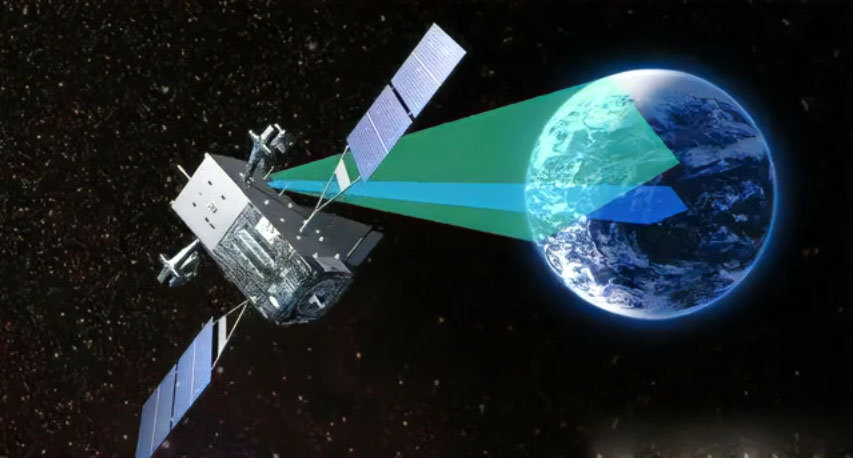
\includegraphics[height=.26\linewidth]{images/遥感1}
        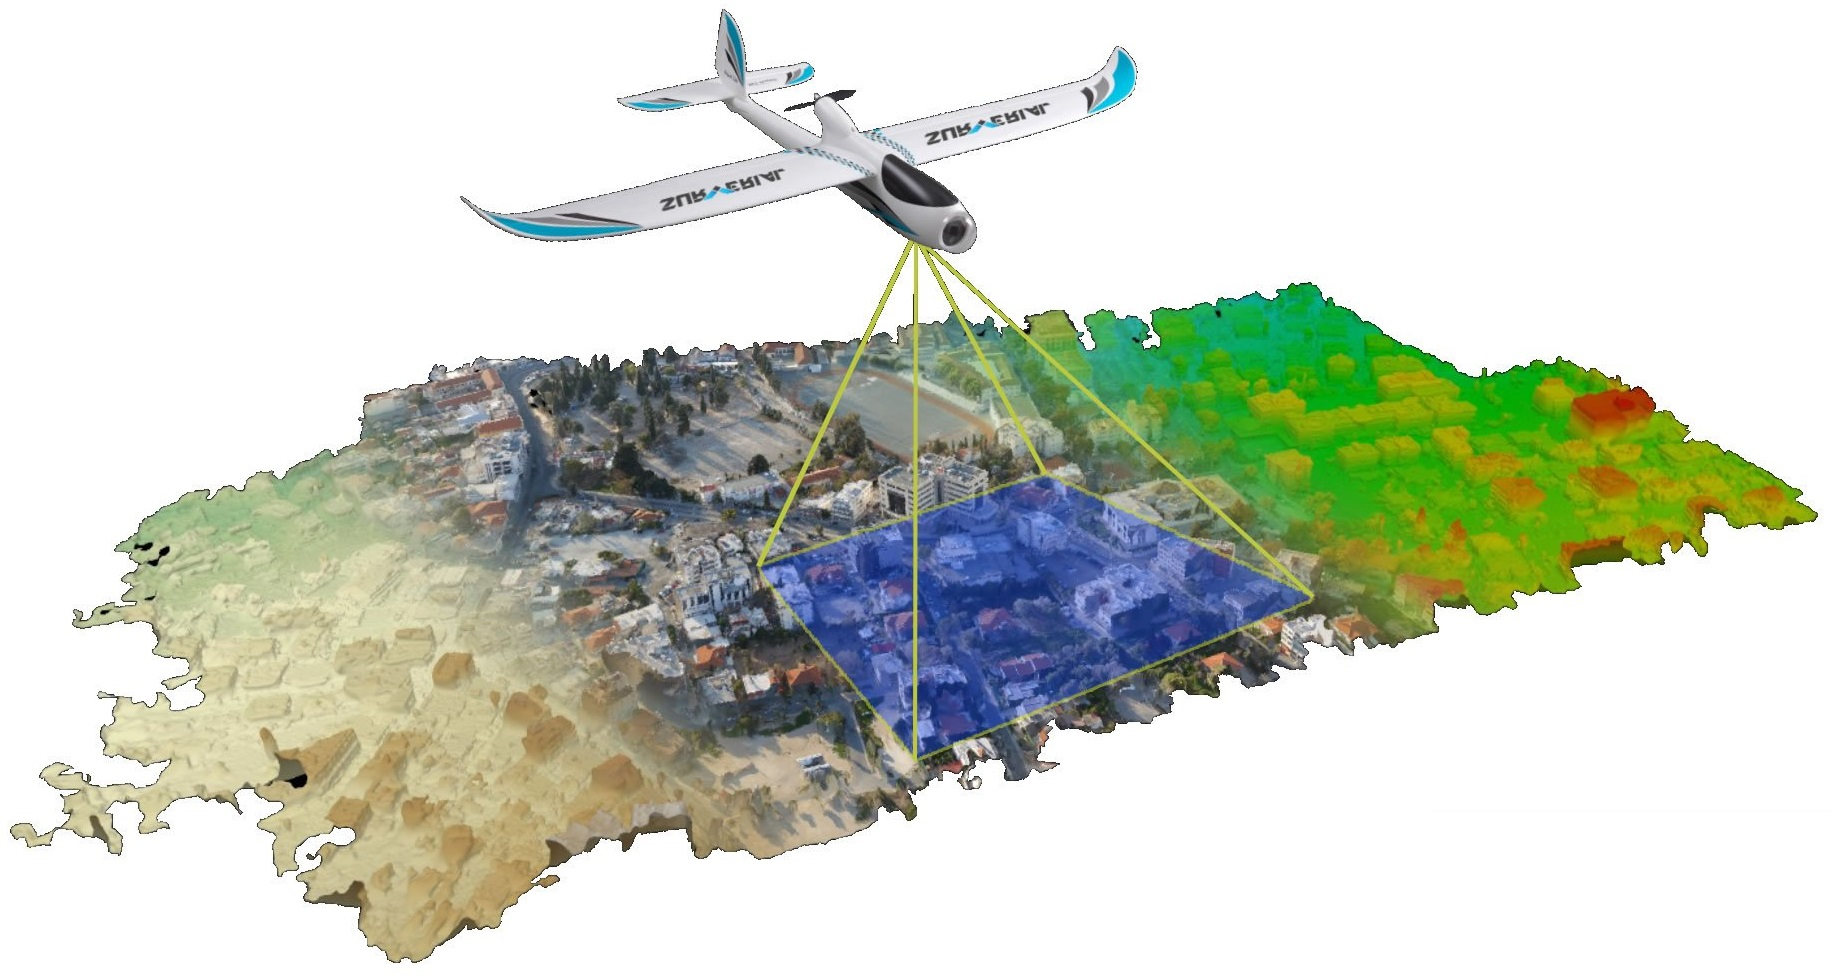
\includegraphics[height=.26\linewidth]{images/遥感2}
    \end{figure}

\end{frame}

\begin{frame}
    \frametitle{遥感技术原理}
    \begin{figure}[htpb]
        \centering
        {\bfseries 不同地物对电磁波辐射、反射、吸收的特性不同 \qquad}
        \smallskip

        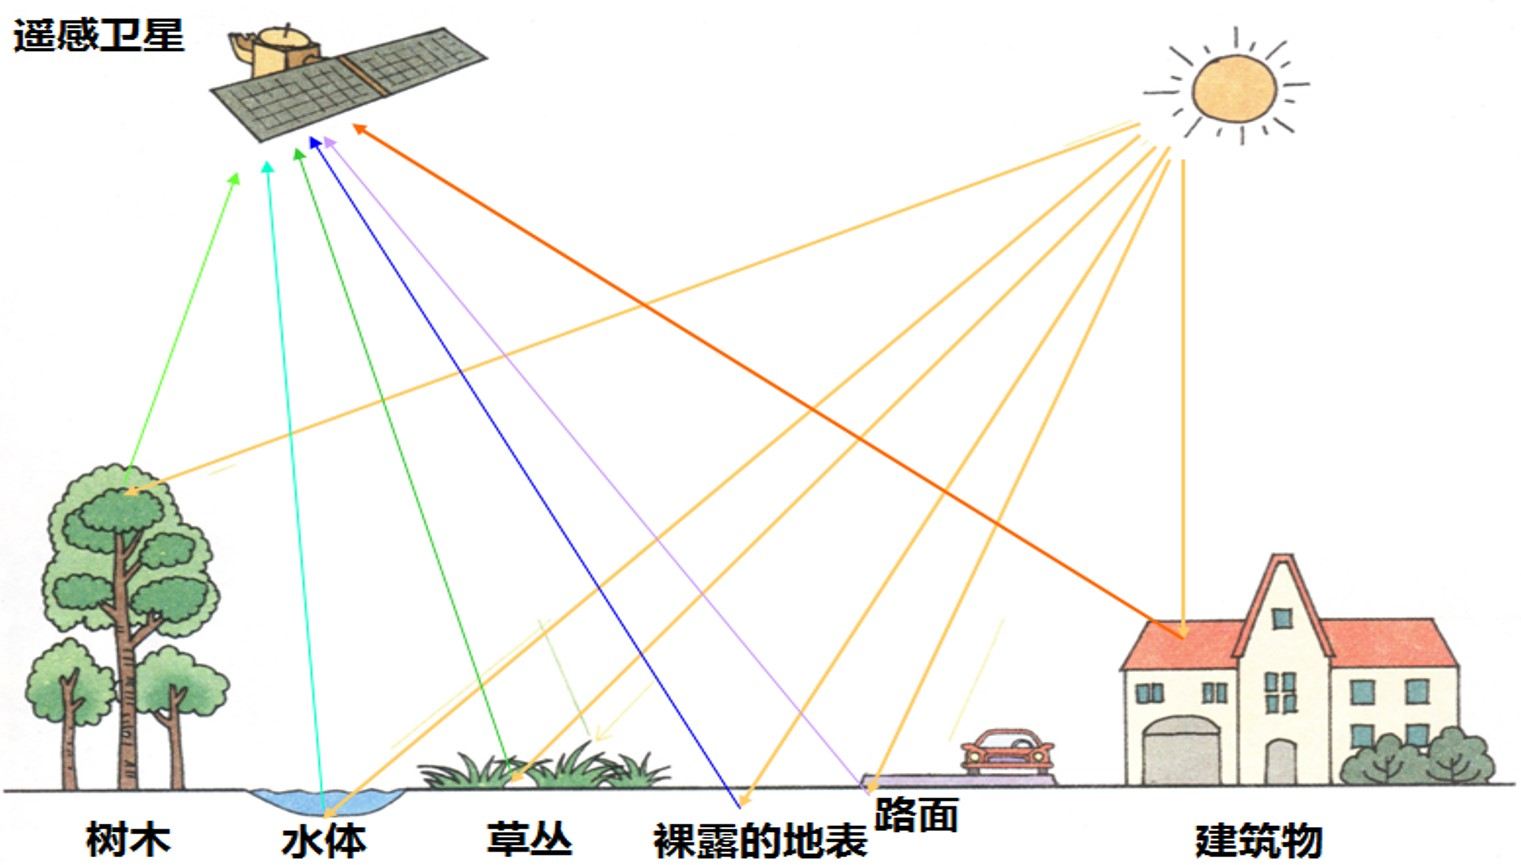
\includegraphics[height=.4\linewidth]{images/遥感原理}
    \end{figure}
\end{frame}
%  遥感之所以能苟根据收集到的电磁波信息来识别地物目标，是因为有信息源的存在。信息源是遥感探测的依据，任何物体都具有发射、反射和吸收电磁波的特性，目标地物与电磁波之间的相互作用构成物体的电磁波特性。因此，遥感技术主要是建立在物体辐射和反射电磁波的原理之上。目标物体的电磁波特性由传感器来获取，通过返回舱或微波天线传至地面接受站。地面接收站将接收到的信息进行存储和处理，转换成用户可以使用的各种数据格式。用户再按照不同的应用目的对这些信息进行分析处理，以达到遥感应用的目的。

\begin{frame}
    \frametitle{遥感系统组成}
    \begin{figure}[htpb]
        \centering
        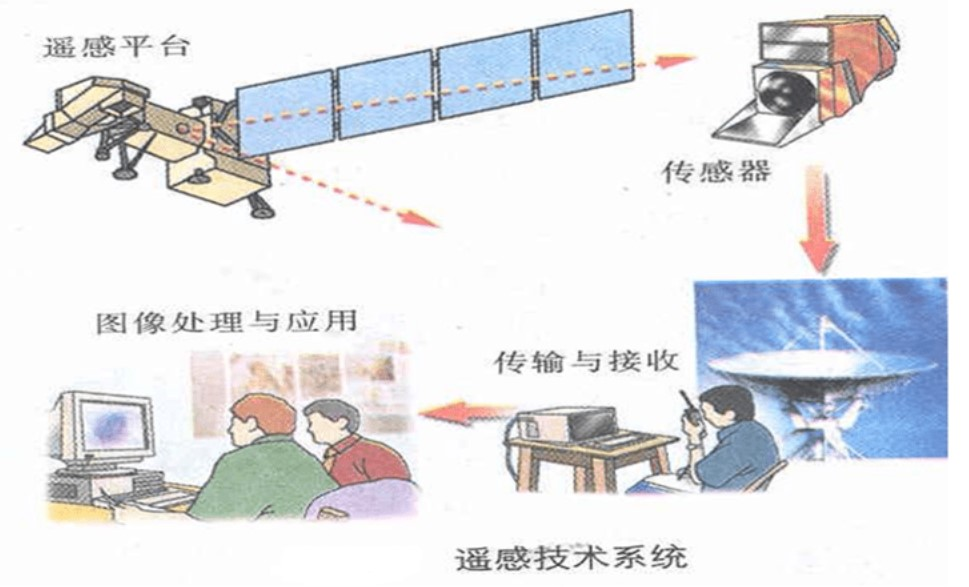
\includegraphics[height=.44\linewidth]{images/遥感组成}
    \end{figure}
\end{frame}

\begin{frame}
    \frametitle{遥感图像}
    \begin{figure}[htpb]
        \centering
        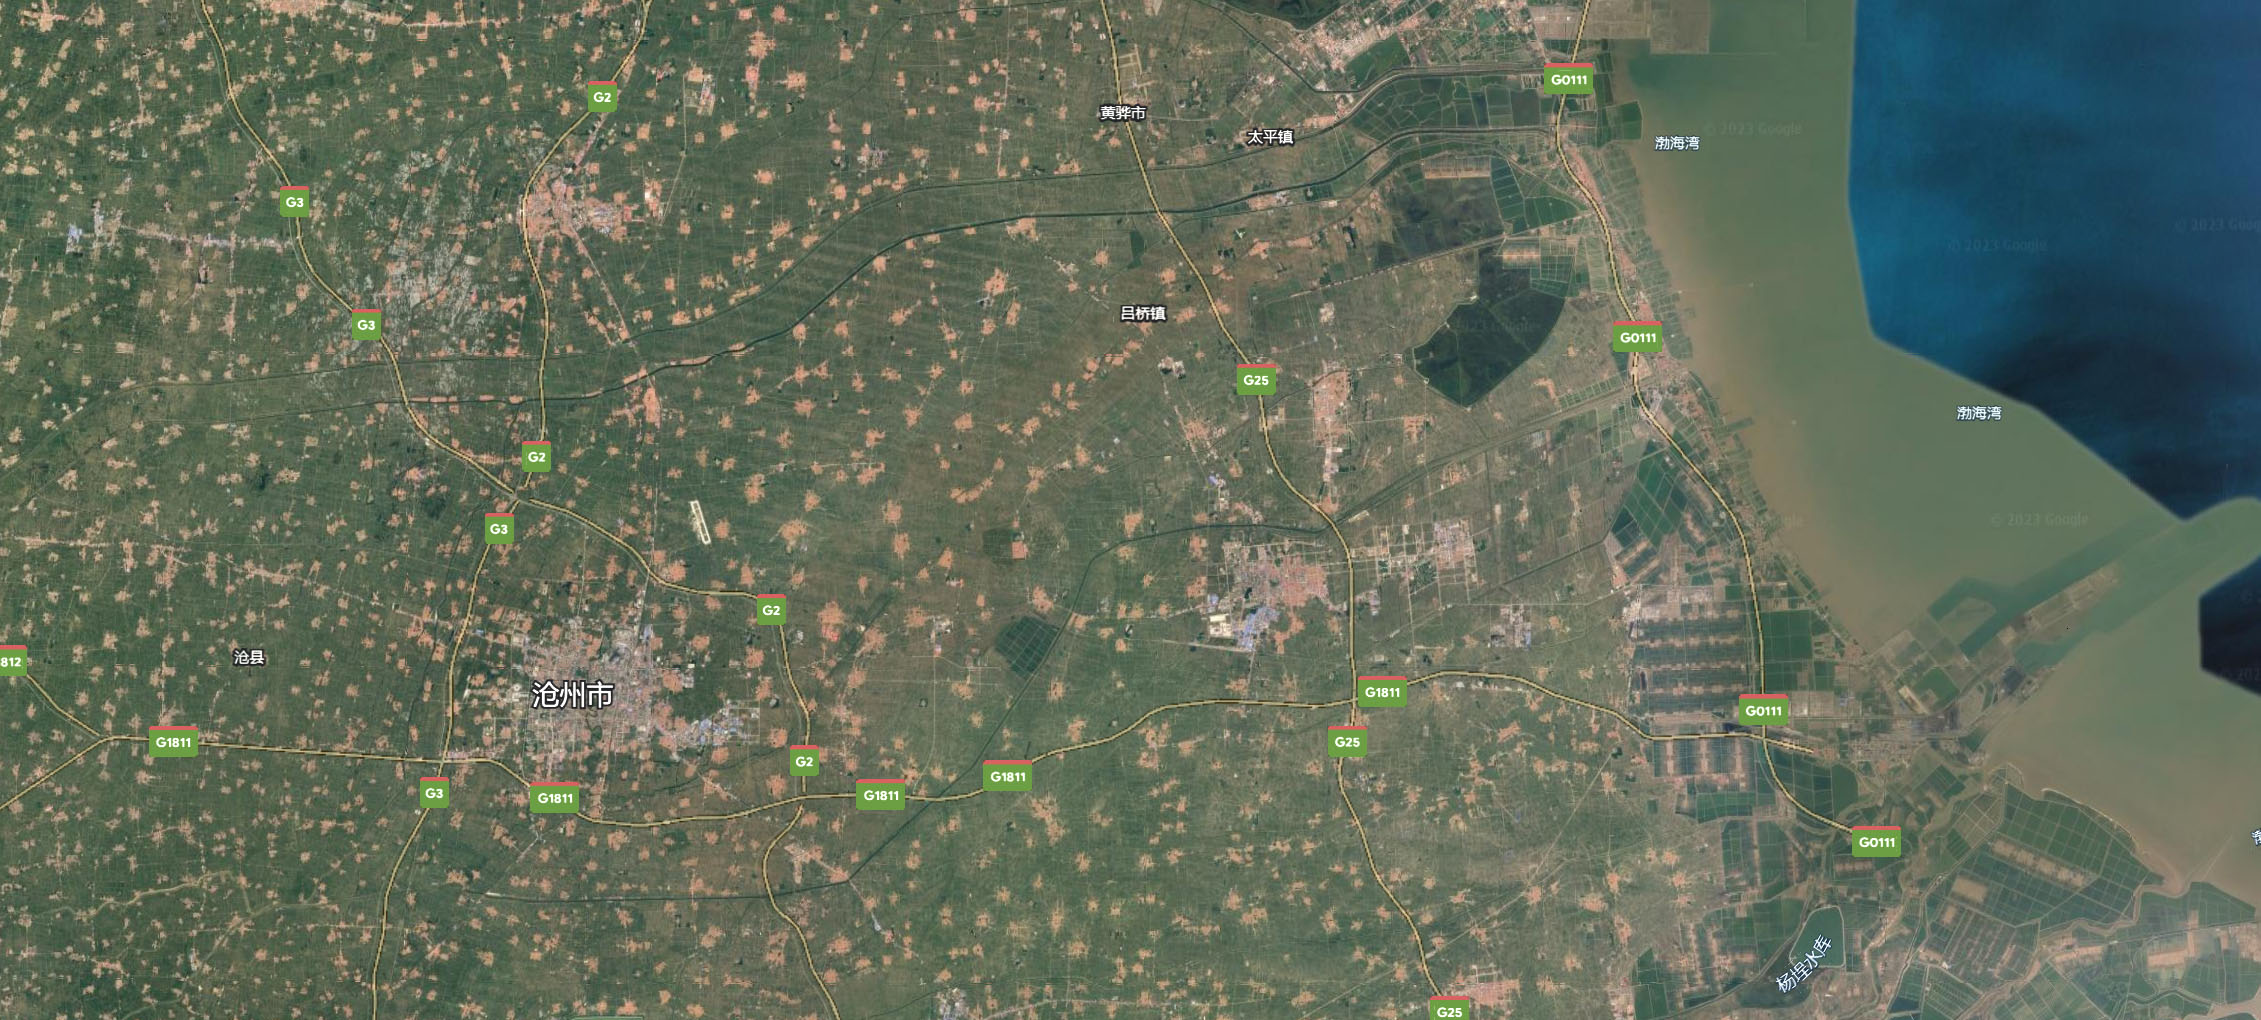
\includegraphics[height=.44\linewidth]{images/遥感图像2}
    \end{figure}
\end{frame}

\begin{frame}
    \frametitle{遥感图像}
    \begin{figure}[htpb]
        \centering
        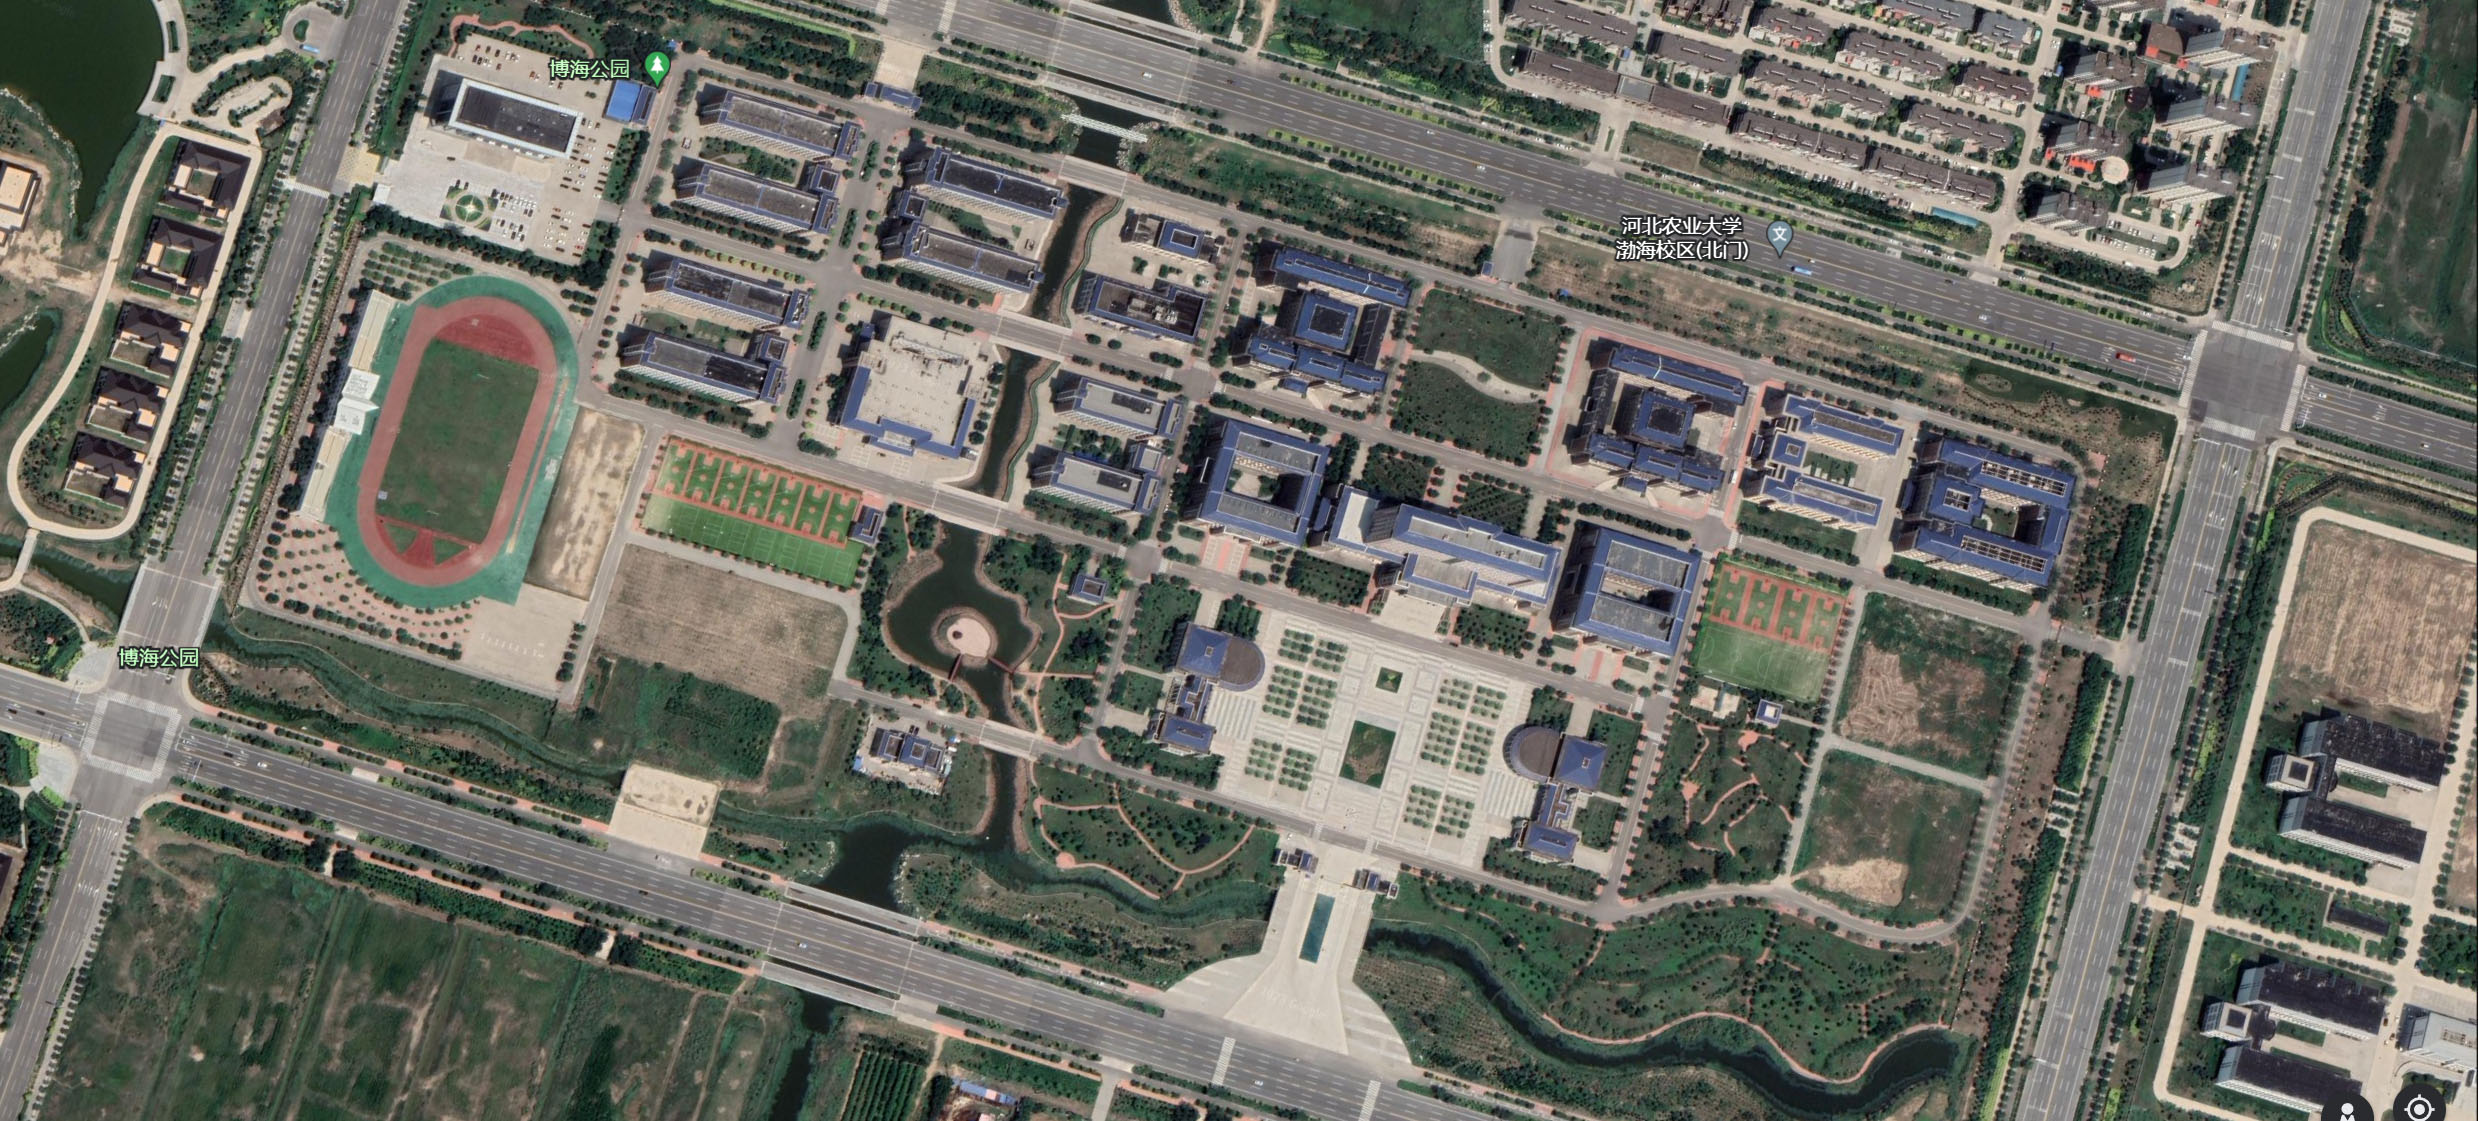
\includegraphics[height=.44\linewidth]{images/遥感图像}
    \end{figure}
\end{frame}


\begin{frame}
    \frametitle{遥感的分类}
    按遥感平台的高度分类大体上可分为航天遥感、航空遥感和地面遥感。
    \Large{
        \begin{itemize}
            \item {\cbf{天}} \qquad \faSatellite \quad \faIcon{space-shuttle} \quad \faIcon{rocket}
            
            \item {\cbf{空}} \qquad \faIcon{plane} \quad \faIcon{helicopter} \quad \faIcon{parachute-box} 
            \item {\cbf{地}} \qquad \faIcon{truck-monster} \quad \faIcon{ship} \quad \faIcon{archway}
            
            \item {\cbf{其它}} \quad \faIcon{internet-explorer} \quad\faIcon{people-arrows} 
        \end{itemize}}
\end{frame}


\begin{frame}
    \frametitle{天宫空间站}
    \begin{figure}[htpb]
        \centering
        
\includegraphics[width=.8\linewidth]{空间站}
    \end{figure}
    \vspace{-4pt}
\end{frame}


\begin{frame}
    \frametitle{天宫空间站}
    \newcommand{\foo}{\color{maincolor}\makebox[0pt]{\textbullet}\hskip-0.5pt\vrule width 1pt\hspace{\labelsep}}
    \begin{table}
        \centering
        \renewcommand\arraystretch{1.4}\arrayrulecolor{maincolor}
        \begin{tabular}{@{\,}r <{\hskip 2pt} !{\foo} >{\raggedright\arraybackslash}p{.8\linewidth}}
        2010.9 & 中央专门委员会批准实施载人空间站工程 \\
        2012.3 & 天宫空间站完成了立项综合论证转入方案设计阶段 \\
        2014.6 & 天宫空间站结束方案设计阶段工作转入初样研制阶段 \\
        2021.4 & 天和核心舱发射 \\
        2021.6 & 神舟十二号发射，聂海胜、刘伯明、汤洪波首批入驻中国空间站\\
        2022.7 & 问天实验舱发射 \\
        2022.10 & 梦天实验舱发射 \\
        2022.12 & 中国国家主席习近平在新年贺词中宣布，“中国空间站全面建成” \\
        \end{tabular}
    \end{table}
\end{frame}


\begin{frame}
    \frametitle{2024年6月，嫦娥六号任务取得圆满成功}
    \begin{figure}[htpb]
        \centering
        
\includegraphics[width=.9\linewidth]{嫦娥六号}
    \end{figure}
\end{frame}


\begin{frame}
    \frametitle{各国探月计划}
    \vspace{-0.5em}
    \begin{figure}[htpb]
        \centering
        \setcounter{subfigure}{0}
        \subfloat[中国探月计划]{
\includegraphics[height=6.5cm]{中国探月}}\quad
        \subfloat[世界各国探月计划]{
\includegraphics[height=6.5cm]{世界探月}}
    \end{figure}
\end{frame}


\begin{frame}
    \frametitle{中国探月工程}
    \newcommand{\foo}{\color{maincolor}\makebox[0pt]{\textbullet}\hskip-0.5pt\vrule width 1pt\hspace{\labelsep}}
    \begin{table}
        \centering
        \renewcommand\arraystretch{1.4}\arrayrulecolor{maincolor}
        \begin{tabular}{@{\,}r <{\hskip 2pt} !{\foo} >{\raggedright\arraybackslash}p{.8\linewidth}}
        2004 & 中国正式开展月球探测工程 \\
        2007.10 & 嫦娥一号成功发射 \\
        2010.10 & 嫦娥二号发射 \\
        2013.12 & 嫦娥三号着陆月面\\
        2018.12 & 嫦娥四号，人类第一个着陆月球背面的探测器 \\
        2020.12 & 嫦娥五号返回器携带月球样品返回地球 \\
        2024.6 & 嫦娥六号采集月球背面样品1935.3克 \\
        \end{tabular}
    \end{table}
\end{frame}


\begin{frame}
    \frametitle{遥感的分类}
    \begin{itemize}
      \item 按所利用的电磁波的光谱段分类：
        \begin{itemize}
            \item 可见反射红外遥感
            \item 热红外遥感
            \item 微波遥感
        \end{itemize}
      \item 按研究对象分类：
        \begin{itemize}
            \item 资源遥感
            \item 环境遥感
        \end{itemize}
      \item 按应用空间尺度分类：
        \begin{itemize}
            \item 全球遥感
            \item 区域遥感
            \item 城市遥感
        \end{itemize}    
    \end{itemize}
\end{frame}


\begin{frame}
    \frametitle{无人机遥感及其优势}
    以无人机为平台，负载数码相机、数码摄录机等数字遥感设备进行拍摄和记录，通过数据处理技术进行影像的同步传输，实现对地理信息的实时调查与监测。
    \begin{enumerate}
      \item 响应能力快：无人机的低空飞行便于空域申请，同时也降低了对天气条件的要求。升空准备时间短、操作相对简单。
      \item 图像分辨率高：无人机遥感可获取到超高分辨率数字影像和定位数据，可针对特殊监测目标搭载全色波段、单波段、多波段等传感器，也可以进行多角度摄影。
      \item 应用拓展能力强：系统为多种小型遥感传感器提供了多个搭载平台，如探地雷达、热成像仪、SAR等，便于扩展监测功能。
      \item 运营成本低：系统的置建费成本较低，运营成本、维护成本和操作人员的成本要低于载人机系统。
    \end{enumerate}

\end{frame}


\begin{frame}
    \frametitle{大疆---无人机市场引领者\link{https://www.dji.com/cn}}
    \begin{figure}[htpb]
        \centering
        \setcounter{subfigure}{0}
        \subfloat[消费级]{
\includegraphics[height=4cm]{消费级}}\hfill
        \subfloat[专业级]{
\includegraphics[height=4cm]{专业级}}\hfill
        \subfloat[农业无人机]{
\includegraphics[height=4cm]{农业}}
    \end{figure}
\end{frame}

\begin{frame}
    \frametitle{遥感技术在农业中的应用}
    \begin{enumerate}
      \item {\cbf{作物种植面积与长势监测}}
      
      由于不同的作物在遥感影像上呈现不同的颜色、纹理、形状等特征信息，运用卫星与无人机遥感技术获取的遥感影像，利用信息提取的方法，提取作物的种植区域，可快速、大面积获得田间作物种植面积与分布数据。此外，遥感影像还可以实时记录作物不同阶段的生长状况，获得同一地点时间序列的图像了解不同生育阶段的作物长势。% 传统的人工测量，耗时长，效率低。田间调查取样一个小时，只能完成200亩左右。
      \item {\cbf{作物病虫害监测}}
      
      植被对诸如病虫害、肥料缺乏等胁迫的反应随胁迫的类型和程度的不同而变化，相应的，植物特征吸收曲线特别是红色区和红外区的光谱特性就会发生相应变化，所以在病害早期就可通过遥感探测到。% https://zhuanlan.zhihu.com/p/269850549
      \item {\cbf{作物遥感估产 \link{http://www.gov.cn/xinwen/2022-12/12/content_5731454.htm}}}
      
      利用现场测产与遥感卫星数据，建立遥感测产模型，就可以完成对作物的估产，估产结果准确率通常在90\%以上。
    \end{enumerate}
\end{frame}

\begin{frame}
    \frametitle{地理信息系统 GIS}
    地理信息系统（Geographic Information System）是一种特定的十分重要的空间信息系统。它是在计算机硬、软件系统支持下，对整个或部分地球表层（包括大气层）空间中的有关地理分布数据进行采集、储存、管理、运算、分析、显示和描述的技术系统。

    GIS技术把地图这种独特的视觉化效果和地理分析功能与一般的数据库操作集成在一起。

\end{frame}

\begin{frame}
    \frametitle{国家地理信息公共服务平台 \link{https://www.tianditu.gov.cn/}}
    \begin{figure}[htpb]
        \centering
        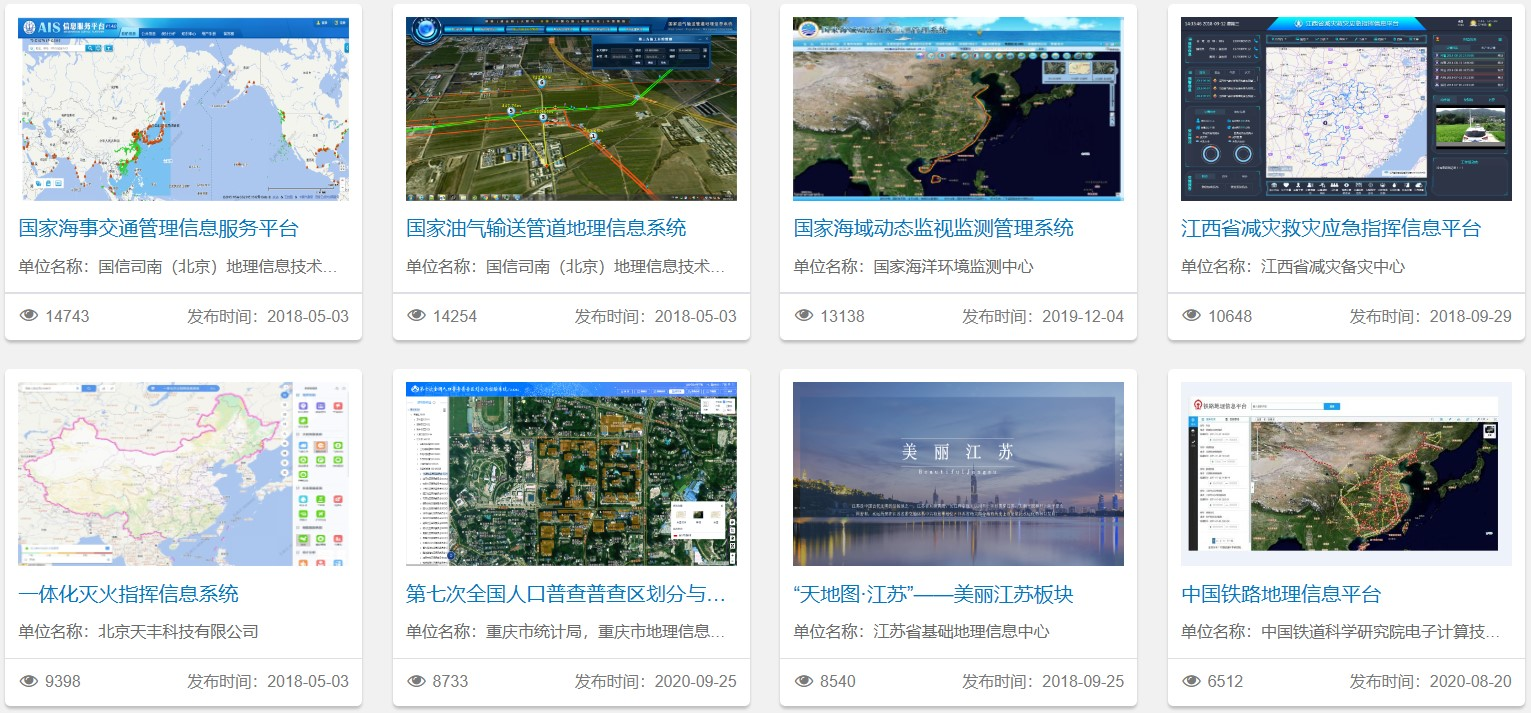
\includegraphics[height=.44\linewidth]{images/天地图}
    \end{figure}
\end{frame}

\begin{frame}
    \frametitle{粮食产量}
    \begin{figure}[htpb]
        \centering
        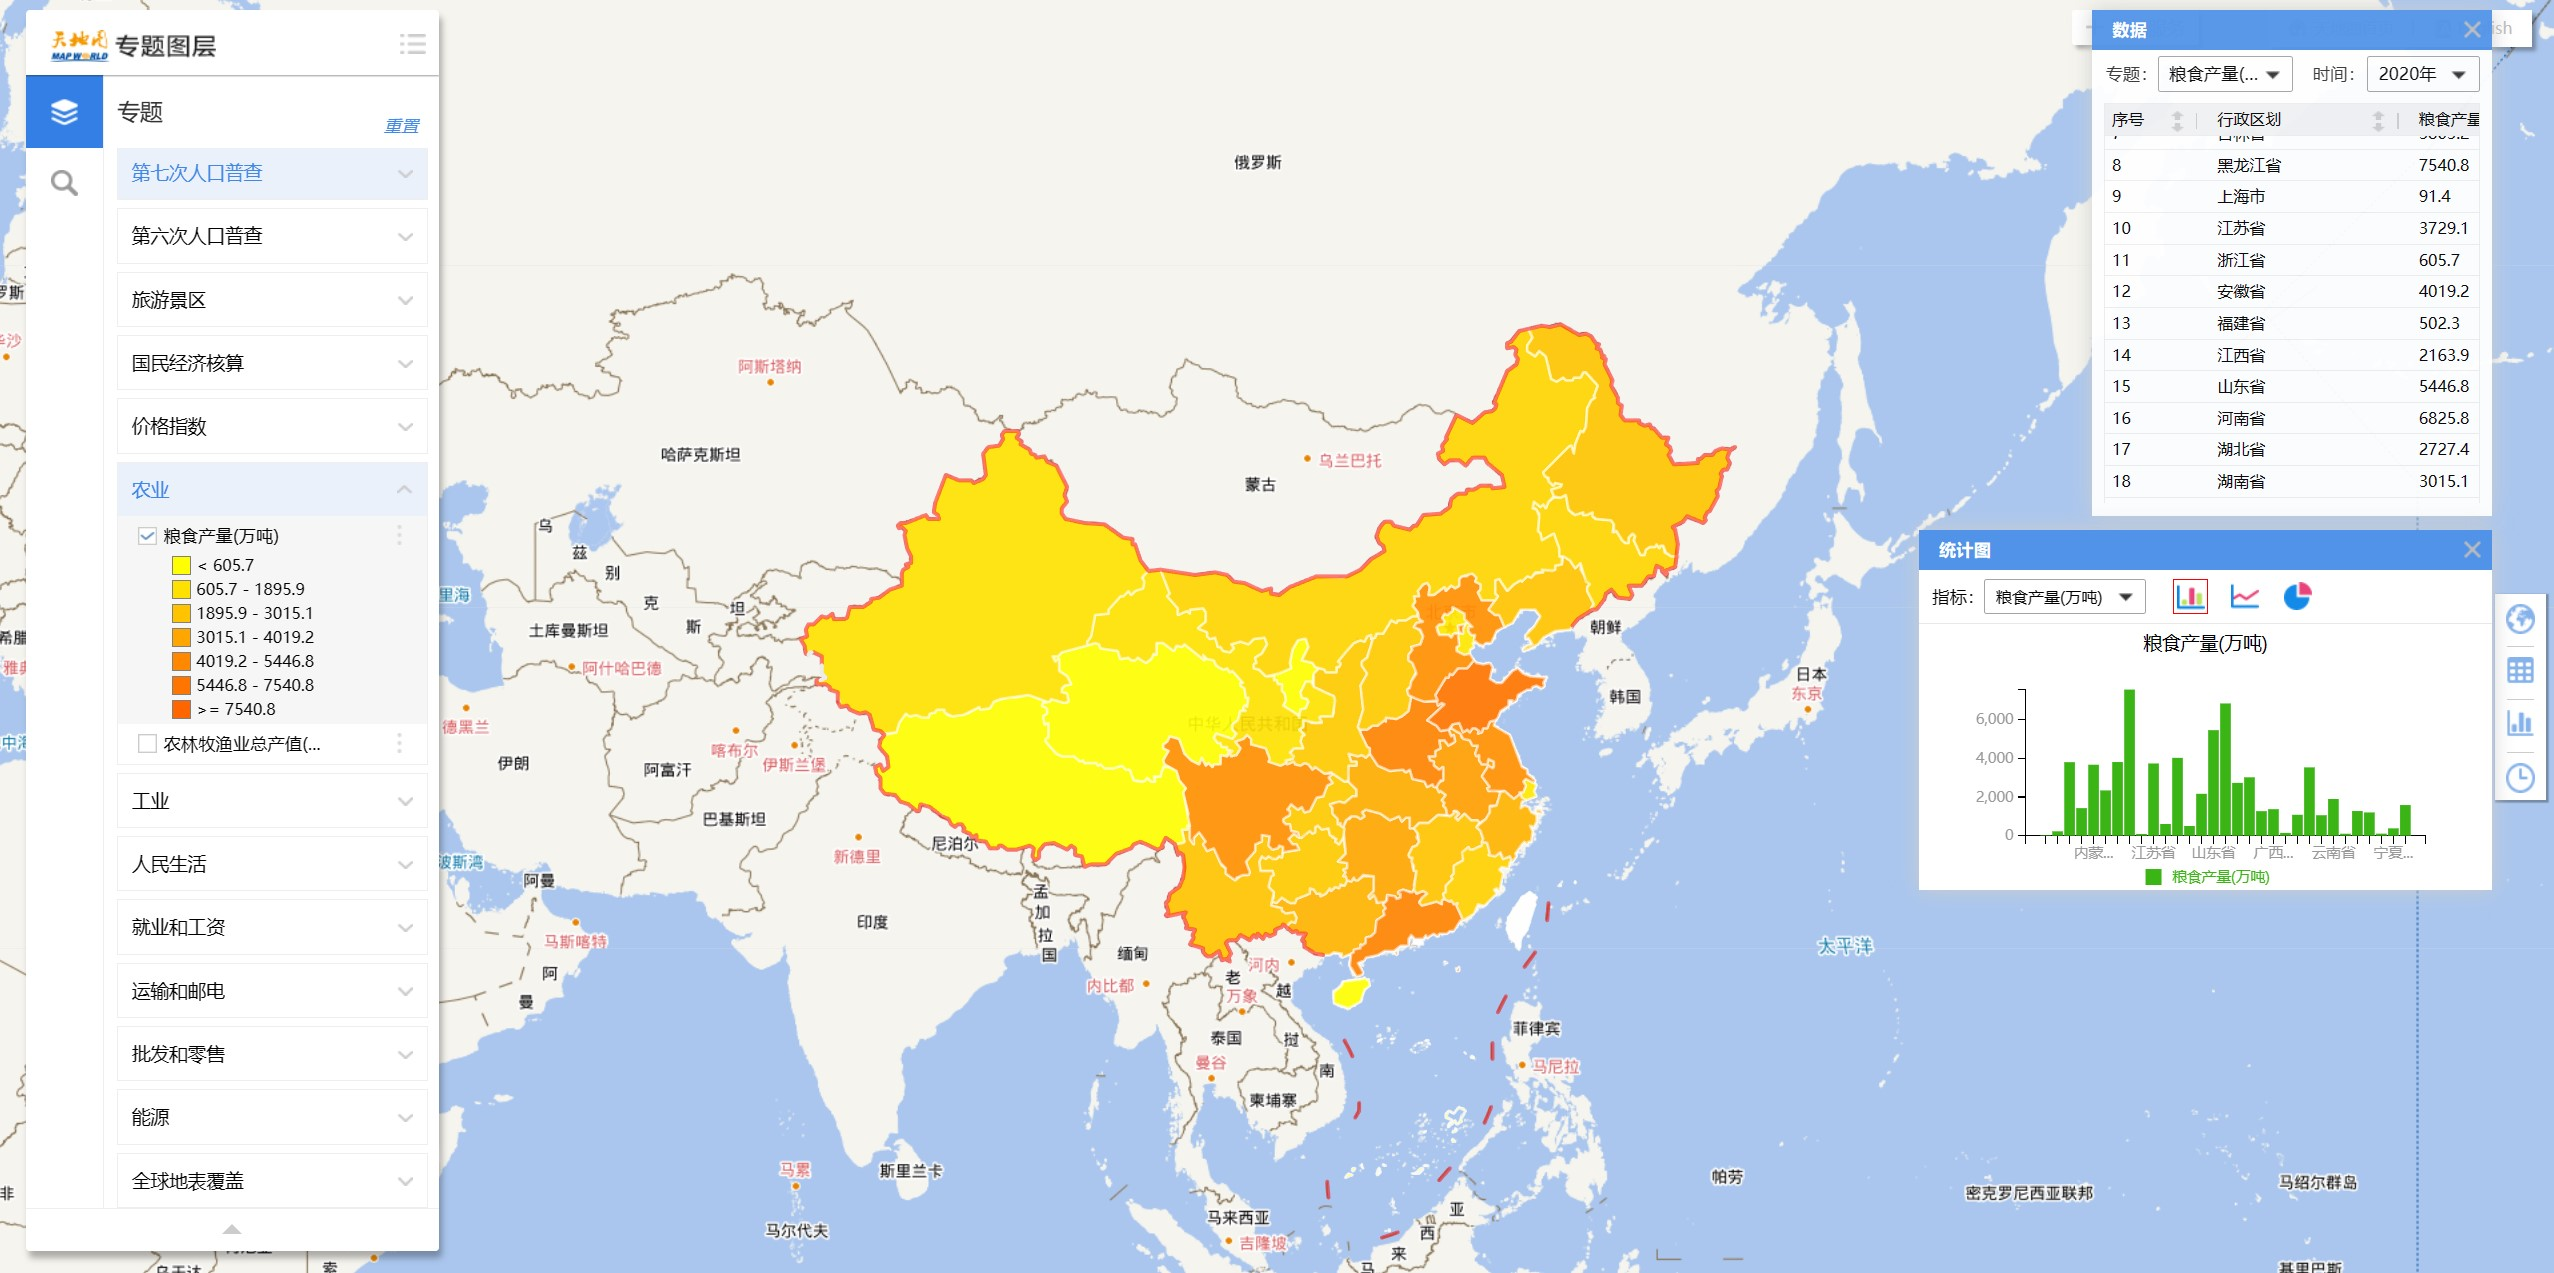
\includegraphics[height=.44\linewidth]{images/粮食产量}
    \end{figure}
\end{frame}

\begin{frame}
    \frametitle{第七次人口普查}
    \begin{figure}[htpb]
        \centering
        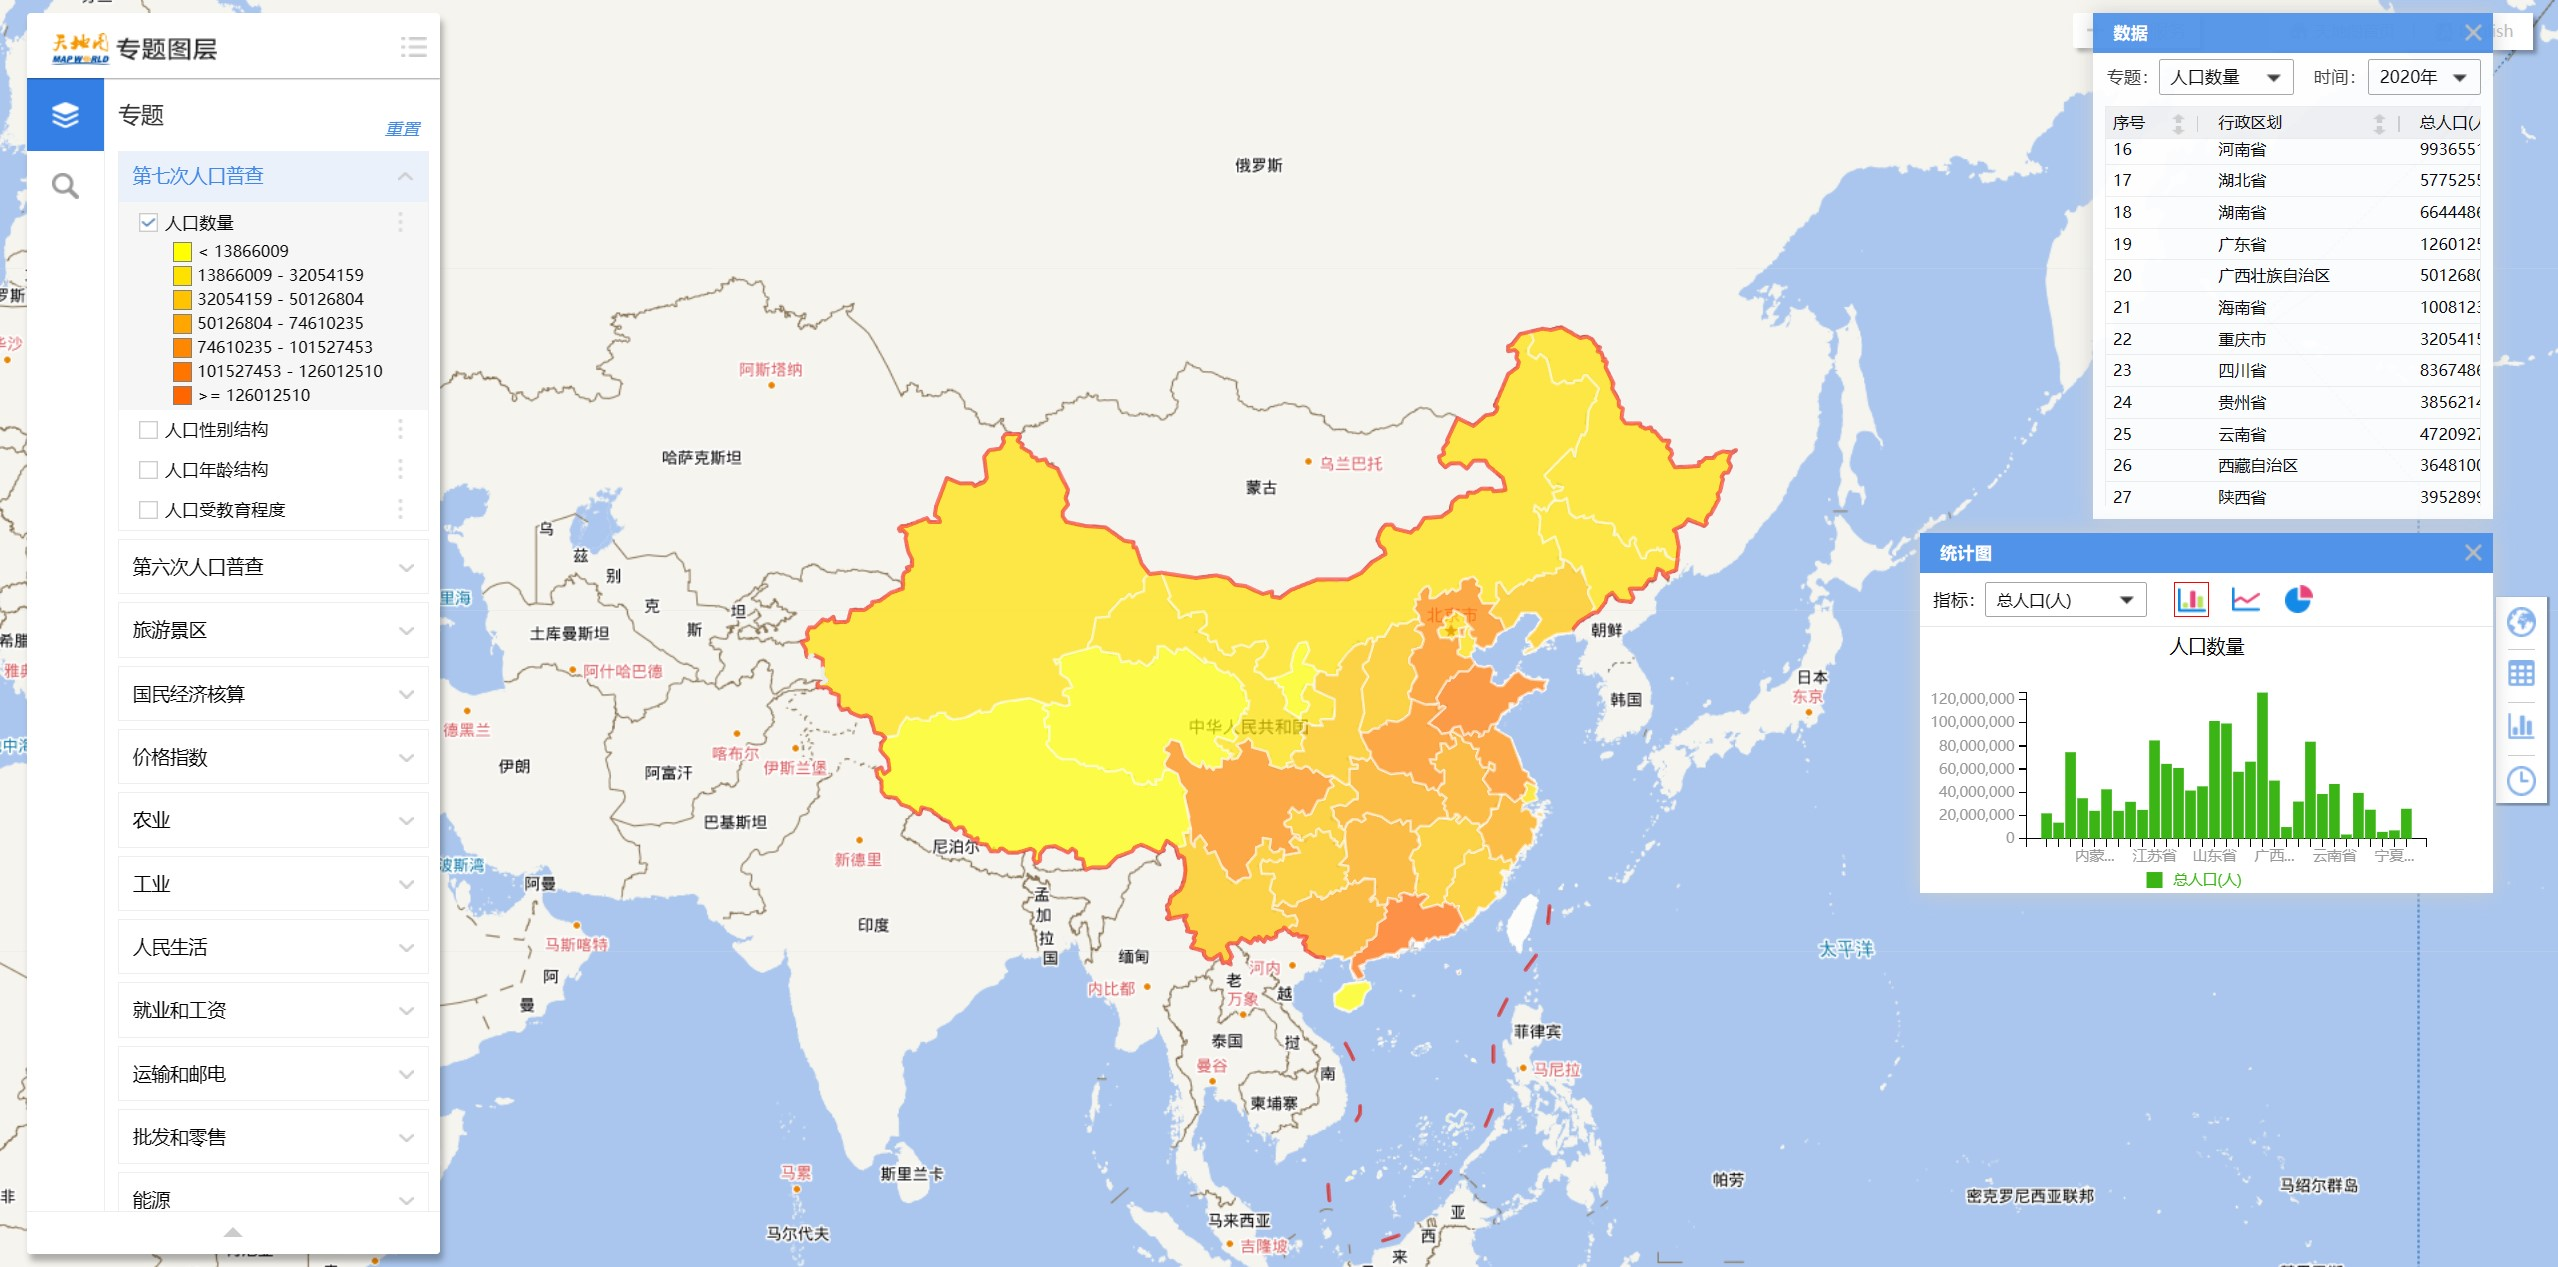
\includegraphics[height=.42\linewidth]{images/人口普查}
    \end{figure}
\end{frame}


\begin{frame}
    \frametitle{GPS与GIS的集成与应用}
    利用GIS中的电子地图和GPS接收机的实时差分定位技术，可以组成GPS+GIS的各种自动电子导航系统，也可以利用GPS的方法对GIS进行实时更新。
    \begin{itemize}
      \item 交通指挥调度
      \item 公安侦破
      \item 车船自动驾驶
      \item 农田作业管理
      \item 渔船捕鱼
    \end{itemize}
\end{frame}


\begin{frame}
    \frametitle{RS与GIS的集成与应用}
    RS是GIS重要的数据源和数据更新的手段，而反过来，GIS则是遥感中数据处理的辅助信息。两者集成可用于：
    \begin{itemize}
      \item 全球变化监测
      \item 农业收成面积监测
      \item 产量预估
      \item 空间数据自动更新
    \end{itemize}
\end{frame}


\begin{frame}
    \frametitle{GPS与RS的集成与应用}
    在遥感平台上安装GPS可以记录传感器在获取信息瞬间的空间位置数据，直接用于空三平差加密，可以大大减少野外控制测量的工作量。
    \begin{itemize}
      \item 自动定时数据采集
      \item 环境监测
      \item 灾害预测
    \end{itemize}

\end{frame}

\begin{frame}
    \frametitle{3S技术在农业中的应用}
        \begin{minipage}{0.68\linewidth}
            \begin{itemize}
                \item {\cbf{农田信息可视化}}
                
                通过各种离散空间数据的采集和GPS传感器的计算，完成对各种田间信息图形化处理。如病虫灾害覆盖图、耕地地力等级图、农作物产量分布图以及农业气候区划图等。
                \item {\cbf{农业生态环境研究}}
                
                地理信息系统广泛应用于农业生态环境研究的多个场景，包括环境监测、生态环境质量评价与环境影响评价、环境预测规划与生态管理以及面源污染防治等。
              \end{itemize}
        \end{minipage}\hfill
        \begin{minipage}{0.28\linewidth}
            \begin{figure}[htpb]
                \centering
                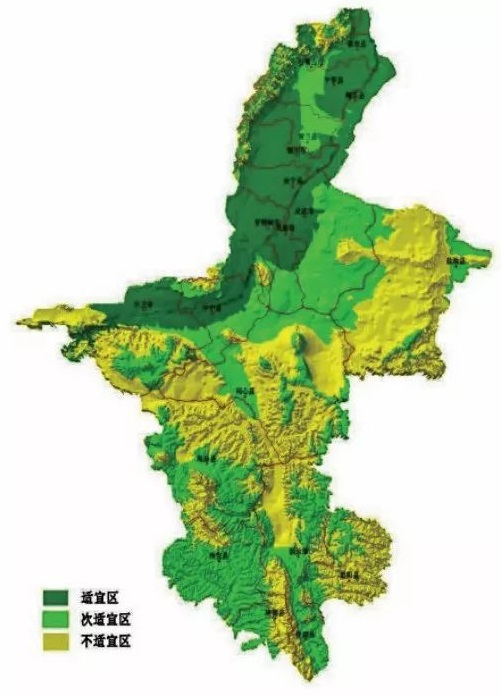
\includegraphics[width=\linewidth]{images/宁夏春小麦气候区划图}
                \caption{宁夏春小麦气候区划图}
            \end{figure}
        \end{minipage}
    
\end{frame}

\begin{frame}
    \frametitle{3S技术在农业中的应用}
    \begin{figure}[htpb]
        \centering
        \setcounter{subfigure}{0}
        \subfloat[土壤采样]{
\includegraphics[height=3cm]{土壤采样}}\hfill
        \subfloat[农田三维地形测量]{
\includegraphics[height=3cm]{农田三维地形测量}}\hfill
        \subfloat[农作物不同生育期长势监测]{
\includegraphics[height=3cm]{长势监测}}
    \end{figure}
\end{frame}

\begin{frame}
    \frametitle{3S技术集成应用-农业无人机 \link{https://ag.dji.com/cn/t50}}
        \begin{minipage}{0.58\linewidth}
            \begin{center}
                {\bfseries 智慧农业生态系统}
            \end{center}
            通过大疆智慧农业平台和全新 Mavic 3M 航测无人机，即可实现自动巡田、土地平整监测、出苗识别、长势分析、处方图变量作业等智慧农业解决方案。依据作物生长情况，结合农田处方图，农业无人飞机即可实现精准变量作业，如水稻变量施肥，棉花变量化控，大豆、玉米变量营养液等。
        \end{minipage}\hfill
        \begin{minipage}{0.38\linewidth}
            \begin{figure}[htpb]
                \centering
                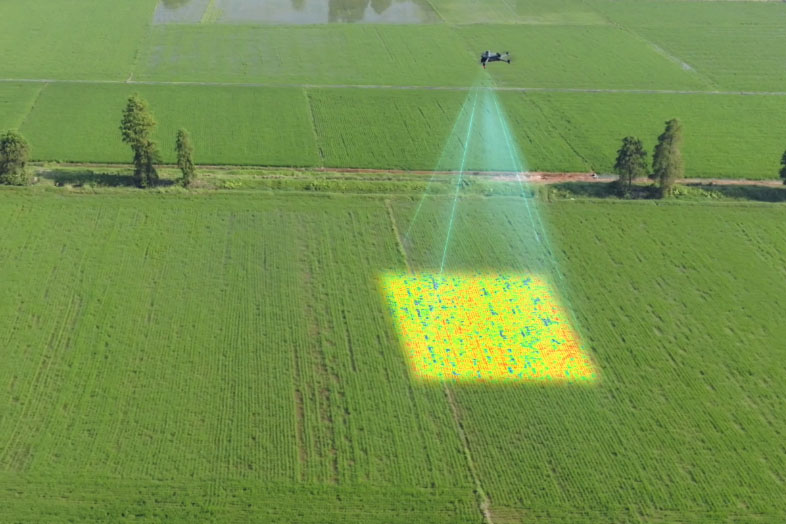
\includegraphics[width=.8\linewidth]{images/Mavic航测} 
                
                ~~~

                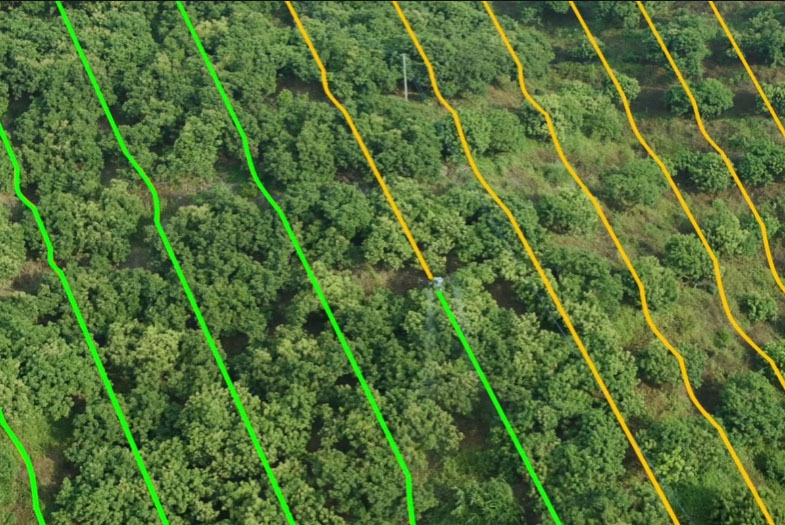
\includegraphics[width=.8\linewidth]{images/Mavic作业}
            \end{figure}
        \end{minipage}
    
\end{frame}


\begin{frame}
    \frametitle{农田测绘：从脚步丈量到无人机测绘}
    \begin{figure}[htpb]
        \centering
        \setcounter{subfigure}{0}
        \subfloat[脚步丈量，携带GPS手持测绘器采集边界的经纬坐标，利用计算机获取农田面积、地理位置等数据信息。]{
\includegraphics[height=3.8cm]{脚步丈量}}\hfill
        \subfloat[无人机测绘，搭载高精度 GNSS RTK 定位模块，航测精度达到了厘米级。]{
\includegraphics[height=3.8cm]{无人机测绘}}
    \end{figure}
\end{frame}


\subsection{条码技术}



\begin{frame}
    \frametitle{条码技术}
    条码技术是在计算机应用和实践中产生并发展起来的广泛应用于商业、邮政、图书管理、仓储、工业生产过程控制、交通等领域的一种自动识别技术，具有输入速度快、准确度高、成本低、可靠性强等优点，在当今的自动识别技术中占有重要的地位。
    \begin{figure}[htpb]
        \centering
        
\includegraphics[height=.18\linewidth]{images/一维条码} \qquad 
        
\includegraphics[height=.22\linewidth]{images/二维码}
    \end{figure}
\end{frame}


\begin{frame}
    \frametitle{一维条码}
    一维条码是由一组规则排列的条、空以及对应的字符组成的标记，\maincolor{“条”指对光线反射率较低的部分，“空”指对光线反射率较高的部分}，这些条和空组成的数据表达一定的信息，并能够用特定的设备识读，转换成与计算机兼容的二进制和十进制信息。通常对于每一种物品，它的编码是唯一的。
    \begin{block}{说一说}
        你在哪些地方见过这样的条码？
        \begin{figure}[htpb]
            \centering
            
\includegraphics[width=.45\linewidth]{一维条码}
        \end{figure}
    \end{block}
\end{frame}


\begin{frame}
    \frametitle{工作原理}        
        \begin{minipage}{0.68\linewidth}
            由于不同颜色的物体，其反射的可见光的波长不同，白色物体能反射各种波长的可见光，黑色物体则吸收各种波长的可见光。条形码扫描仪则是一个可以发射可见光和接收其反射信号的仪器。在读取条形码的时候，它先向条形码发射一组可见光，这一组光照到条形码上，再反射给扫描仪上面的接收器，接收器根据其反射回来的光信号的强弱来识别条形码上的“条”、“空”信息。这些信息组合在一起，最终得到一组数字。
        \end{minipage}\hfill
        \begin{minipage}{0.28\linewidth}
            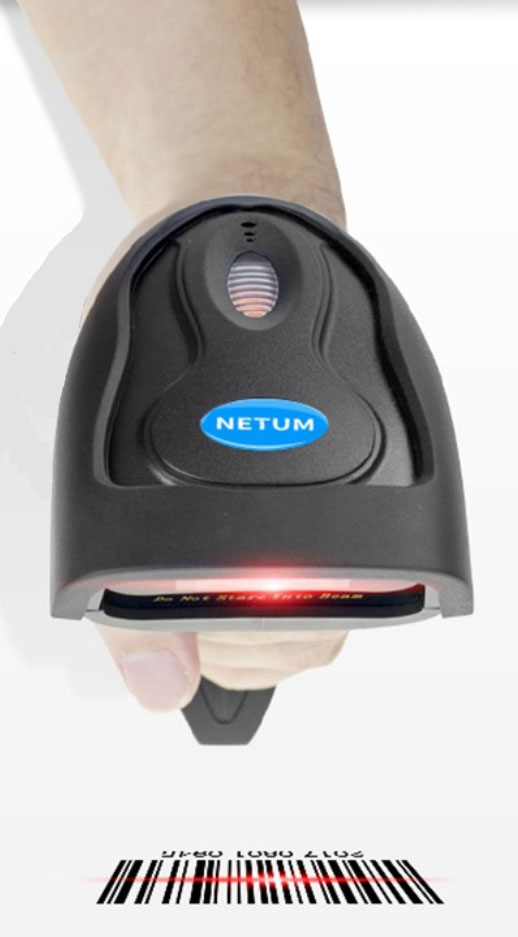
\includegraphics[height=180pt]{images/扫码枪}
        \end{minipage}
\end{frame}


\begin{frame}
    \frametitle{条码技术的特点}
    \begin{enumerate}
      \item 简单
      \item 信息采集速度快
      \item 采集信息量大
      \item 可靠性高
      \item 灵活、实用
      \item 自由度大
      \item 设备结构简单、成本低
    \end{enumerate}
\end{frame}


\begin{frame}
    \frametitle{POS系统}
    POS系统是通过读取产品的EAN码，在超市、便利店里管理销售、仓储和采购的系统。由于该系统也可以提供有关消费者需求趋向的准确资料，可以用来决策管理策略。

    \begin{figure}[htpb]
        \centering
        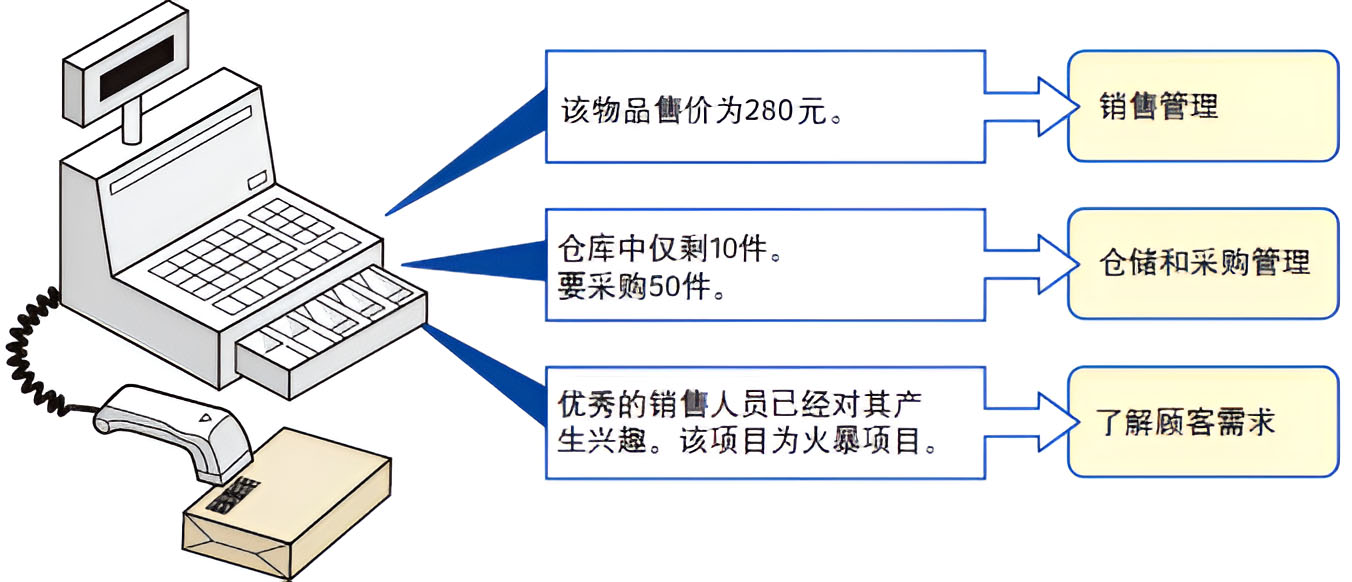
\includegraphics[height=.3\linewidth]{images/POS系统}
    \end{figure}
\end{frame}

\begin{frame}
    \frametitle{EAN码}
    EAN码（European Article Number）是国际物品编码协会制定的一种商品用条码，通用于全世界。EAN码有标准版（EAN-13）和缩短版（EAN-8）两种。
    
    国际条码组织给我国分配的编码从690到699。

    以690、691开头时，厂商识别码为四位，商品项目代码为五位；

    以692、693开头时，厂商识别码是五位，商品项目代码是四位。

    厂商识别代码: 由中国物品编码中心统一向厂商进行分配。

    商品项目代码:由厂商根据有关规定自行分配。

    \begin{figure}[htpb]
        \centering
        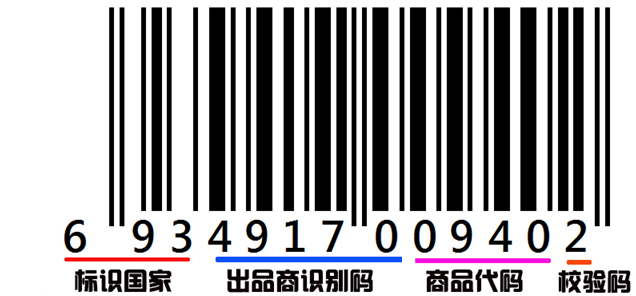
\includegraphics[height=.18\linewidth]{images/EAN码}
    \end{figure}
\end{frame}

\begin{frame}
    \frametitle{国际标准书号ISBN}
        \begin{minipage}{0.38\linewidth}
            \begin{figure}[htpb]
                \centering
                
\includegraphics[height=.7\linewidth]{images/ISBN}
            \end{figure}
        \end{minipage}\hfill
        \begin{minipage}{0.58\linewidth}
            \begin{itemize}
              \item {\bfseries 978} \quad \ \,EAN图书码
              \item {\bfseries 7} \qquad ~\,地区码，7代表中国
              \item {\bfseries 04} \qquad 出版社代码，04为高等教育出版社
              \item {\bfseries 055968} 出版社的图书编号
              \item {\bfseries 2} \qquad ~\,校验码
            \end{itemize}
        \end{minipage}    
\end{frame}

% 2007年1月1日之前，ISBN由10位数字组成，分四个部分：组号（国家、地区、语言的代号），出版者号，书序号和检验码。2007年1月1日起，实行新版ISBN，新版ISBN由13位数字组成，分为5段，即在原来的10位数字前加上3位EAN图书产品代码“978”。最后一位重新校验。
% 前缀 978 989 图书，977期刊
% 第一组号码是国家代码（State Identifier），最短的是一位数字，最长的达五位数字，大体上兼顾文种、国别和地区。把全世界自愿申请参加国际标准书号体系的国家和地区，划分成若干地区，各有固定的编码：美国所出版的书国家代码为0，1代表英语，使用这两个代码的国家有：澳大利亚、加拿大、爱尔兰、新西兰、波多黎各、南非、英国、美国、津巴布韦等；2代表法语，法国、卢森堡以及比利时、加拿大和瑞士的法语区使用该代码；3代表德语，德国、奥地利和瑞士德语区使用该代码；4是日本出版物的代码；5是俄语系国家出版物的代码；7为中国大陆出版物使用的代码等等。国家领域最长可能为5位数字（如不丹为99936），但相对剩下能使用、分配的位数就较为狭隘。
% 第二组号码段
% 第二组号码是出版社代码（Publisher Identifier），由其隶属的国家或地区ISBN中心分配，允许取值范围为2-5位数字。出版社的规模越大，出书越多，其号码就越短。
% 第三组号码段
% 第三组号码是书序码（Title Identifier）由出版社自己给出，而且每个出版社的书序号是定长的（数字9，减去组号、出版社代码所占的位数，就是书序码的位数）。最短的一位，最长的六位。出版社的规模越大，出书越多，书序码越长（如人民文学出版社的出版社代码为02，书序码即为6位，译林出版社代码5447，书序码即为4位）。
% 第四组号码段
% 第四组号码是校验码，其数值由前九位数字依次以10～2加权之和并以11为模计算得到。


\begin{frame}
    \frametitle{条形码的读取}
    条码的黑色条表示二进制的1，白色代表0，而且0.33mm宽度的黑色或者白色条为一个基本的二进制位。有的黑白色条很宽，说明连着好几个二进制1/0。
    \begin{figure}[htpb]
        \centering
        
\includegraphics[width=.48\linewidth]{条形码读取1}
        
\includegraphics[width=.48\linewidth]{条形码读取2}
    \end{figure}
\end{frame}


\begin{frame}
    \frametitle{为什么同一个数字，条码不一样？}
    \qquad EAN码中，每个数字由7个二进制位组成，用黑条代表二进制1，白条代表0。每个数字的二进制表示方法有三个子集：A、B和C。    
\begin{table}[]
    \begin{tabular}{@{}cccccccc@{}}
    \toprule
               & \textbf{A 子集} & \textbf{B 子集} & \textbf{C 子集} & \textbf{}  & \textbf{A 子集} & \textbf{B 子集} & \textbf{C 子集} \\ \midrule
    \textbf{0} & 0001101       & 0100111       & 1110010       & \qquad \textbf{5} & 0110001       & 0111001       & 1001110       \\
    \textbf{1} & 0011001       & 0110011       & 1100110       & \qquad \textbf{6} & 0101111       & 0000101       & 1010000       \\
    \textbf{2} & 0010011       & 0011011       & 1101100       & \qquad \textbf{7} & 0111011       & 0010001       & 1000100       \\
    \textbf{3} & 0111101       & 0100001       & 1000010       & \qquad \textbf{8} & 0110111       & 0001001       & 1001000       \\
    \textbf{4} & 0100011       & 0011101       & 1011100       & \qquad \textbf{9} & 0001011       & 0010111       & 1110100       \\ \bottomrule
    \end{tabular}
    \end{table}
    \qquad 每个数字由两条黑条和两条白条构成，不同宽度的条代表连续的几个0或1。
\end{frame}

\begin{frame}
    \frametitle{根据前置码确定各个数字的编码}
    EAN-13商品条码中的前置码不用条码字符表示。左侧数据符选用A子集还是B子集取决于前置码的数值。右侧数据符及校验符均用字符集中的C子集表示。之所以这样规定，就是可以判断扫描正反，防止扫描错误。
    \bigskip

        \begin{minipage}{0.38\linewidth}
            \begin{figure}[htpb]
                \centering
                
\includegraphics[width=\linewidth]{images/ISBN}
            \end{figure}
        \end{minipage}\hfill
        \begin{minipage}{0.58\linewidth}
            \smallskip

            \begin{table}[]
                \begin{tabular}{@{}ccccccccccc@{}}
                \toprule
                \textbf{前置码} & \textbf{0} & \textbf{1} & \textbf{2} & \textbf{3} & \textbf{4} & \textbf{5} & \textbf{6} & \textbf{7} & \textbf{8} & \textbf{9} \\ \midrule
                \textbf{左1}  & A          & A          & A          & A          & A          & A          & A          & A          & A          & A          \\
                \textbf{左2}  & A          & A          & A          & A          & B          & B          & B          & B          & B          & B          \\
                \textbf{左3}  & A          & B          & B          & B          & A          & B          & B          & A          & A          & B          \\
                \textbf{左4}  & A          & A          & B          & B          & A          & A          & B          & B          & B          & A          \\
                \textbf{左5}  & A          & B          & A          & B          & B          & A          & A          & A          & B          & B          \\
                \textbf{左6}  & A          & B          & B          & A          & B          & B          & A          & B          & A          & A          \\ \bottomrule
                \end{tabular}
                \end{table}
        \end{minipage}

\end{frame}


\begin{frame}
    \frametitle{Code 39，Code 128}
    \qquad 目前国内企业内部自定义码制，可以根据需要确定条码的长度和信息，它编码的信息可以是数字，也可以包含字母，广泛应用在企业内部管理、生产流程、物流控制系统等方面。

    \qquad Code 39 码，是目前 用途广泛的一种条形码，可表示数字、英文字母以及“−”、“.”、“/”、“+”、“\%”、“\$”、 “\ ”（空格）和“*”共 44 个符号，其中“*”仅作为起始符和终止符。

    \qquad CODE128 码可表示从 ASCII 0 到ASCII 127 共128个字符，故称128码。其中包含了数字、字母和符号字符。
    \begin{figure}[htpb]
        \centering
        
\includegraphics[width=.78\linewidth]{images/code128}
    \end{figure}
\end{frame}


\begin{frame}
    \frametitle{二维码}
        \begin{minipage}{0.58\linewidth}
            二维码是条形码的升级，条形码是一维，记录横向信息，不记录纵向。而二维码既记录横向也记录纵向。二维码能在有限的空间内存储更多的信息，并可脱离计算机使用。

            二维码是现在应用最广泛，最受青睐的标签，二维码的应用场景非常多，如对产品进行追溯、通过二维码进行保密管理、通过二维码读取文字信息、条码信息、产品出入库管理、产品防伪等等。
        \end{minipage}\hfill
        \begin{minipage}{0.38\linewidth}
            \begin{figure}[htpb]
                \centering
                
\includegraphics[width=\linewidth]{images/二维码}
            \end{figure}
        \end{minipage}
    
\end{frame}

\begin{frame}
    \frametitle{二维码的种类}
    \begin{itemize}
      \item 矩阵式二维码：Aztec、Maxi Code、QR Code、 Data Matrix等。
      \item 线性堆叠式二维码：Code 16K、Code 49、PDF417等。
    \end{itemize}
    \begin{figure}[htpb]
        \centering
        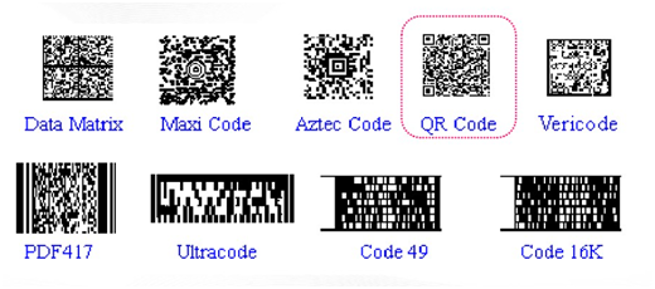
\includegraphics[height=.3\linewidth]{images/二维码种类}
    \end{figure}
\end{frame}

\begin{frame}
    \frametitle{QR码的规格}
    QR码设有1到40的不同版本(种类)，每个版本都具备固有的码元结构(码元数)。

    “码元结构”是指二维码中的码元数。从版本1(21码元×21码元)开始，在纵向和横向各自以4码元为单位递增，一直到版本40(177码元×177码元)。

    \begin{figure}[htpb]
        \centering
        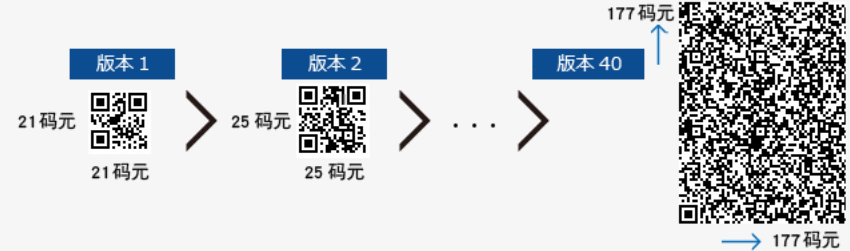
\includegraphics[width=\linewidth]{images/QR码的版本规格尺寸}
    \end{figure}
\end{frame}

\begin{frame}
    \frametitle{QR码的基本结构}
    \begin{figure}[htpb]
        \centering
        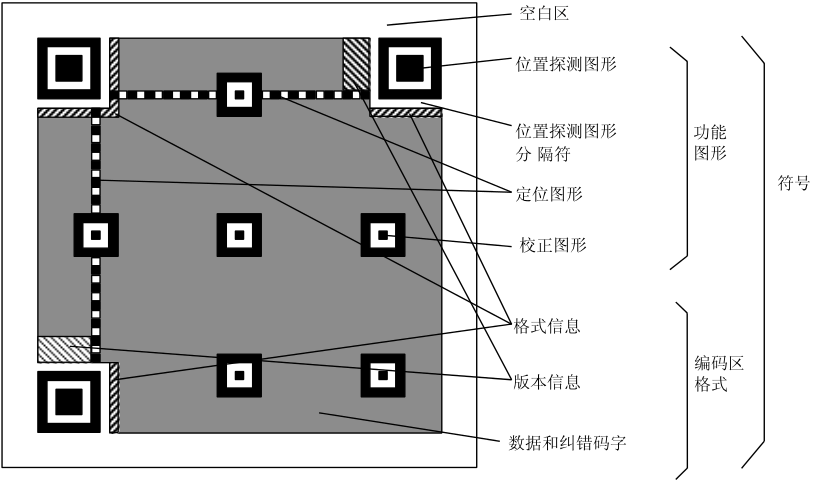
\includegraphics[height=.46\linewidth]{images/QR码的结构}
    \end{figure}
\end{frame}

\begin{frame}
    \frametitle{QR码的特点}
    \begin{itemize}
      \item 存储大容量信息
      \item 支持所有类型的数据
      \item 在小空间内打印
      \item 对变脏和破损的适应能力强
      \item 可以从任意方向读取
      \item 支持数据合并功能
    \end{itemize}
\end{frame}

% 传统的条形码只能处理20位左右的信息量，与此相比，QR码可处理条形码的几十倍到几百倍的信息量。

% 另外，QR码还可以支持所有类型的数据。（如：数字、英文字母、日文字母、汉字、符号、二进制、控制码等）。一个QR码最多可以处理7089字(仅用数字时)的巨大信息量。

% QR码使用纵向和横向两个方向处理数据，如果是相同的信息量，QR码所占空间为条形码的十分之一左右。(还支持Micro QR码，可以在更小空间内处理数据。)

% QR码从360°任一方向均可快速读取。其奥秘就在于QR码中的3处定位图案，可以帮助QR码不受背景样式的影响，实现快速稳定的读取。

% QR码可以将数据分割为多个编码，最多支持16个QR码。使用这一功能，还可以在狭长区域内打印QR码。另外，也可以把多个分割编码合并为单个数据。



\begin{frame}
    \frametitle{二维码应用}
            \begin{itemize}
              \item 移动支付
              \item 加好友，关注公众号
              \item 网站跳转
              \item 产品溯源
              \item 点餐购票
              \item 网站登录
              \item 广告促销
            \end{itemize}
\end{frame}


\begin{frame}
    \frametitle{农产品溯源系统}
    \begin{figure}[htpb]
        \centering
        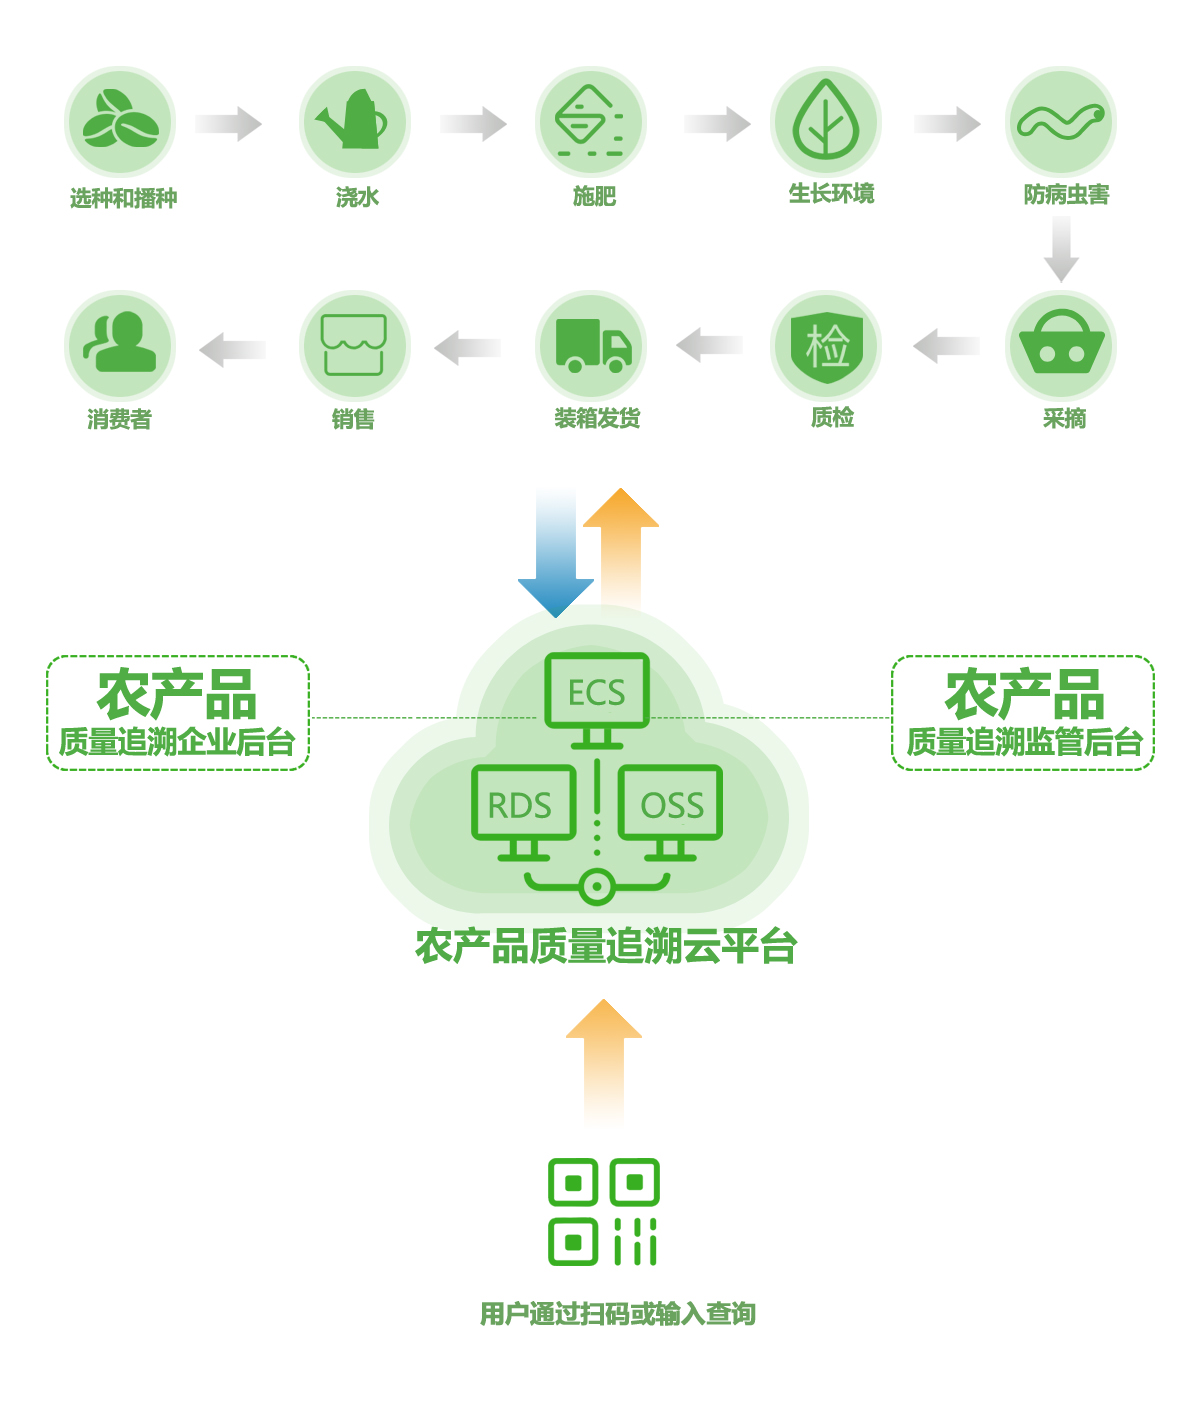
\includegraphics[height=.44\linewidth]{images/农产品溯源}
        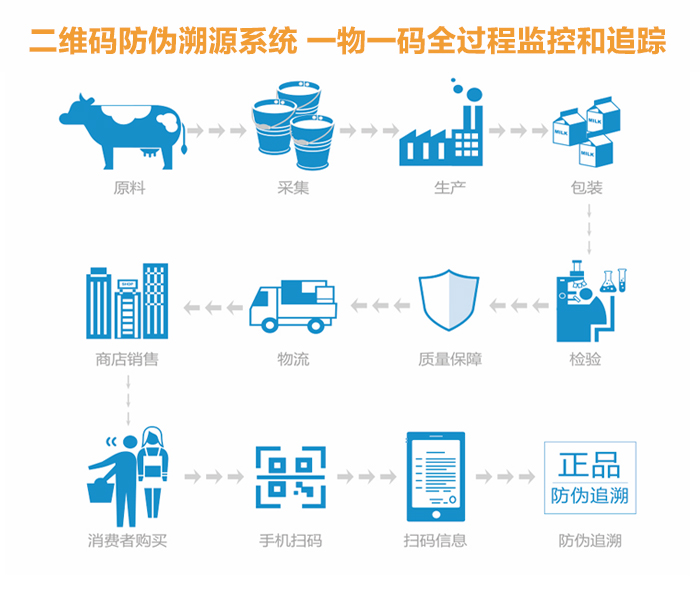
\includegraphics[height=.44\linewidth]{images/农产品溯源2}
    \end{figure}
\end{frame}


\subsection{种植养殖业数字化技术}

\begin{frame}
    \frametitle{种植业数字化技术}
    种植业数字化是数字技术在农作物种植各环节的应用，通过获取、记录农业生产经营各环节数据，并计算分析得出应对方案，为种植各环节流程提供智能决策，提高生产效率。
    \begin{itemize}
      \item {\cbf{数字化“三情”监测分析}} 利用物联网等信息化手段对墒情、苗情、灾情等“三情”和气象进行预测预报，精准指导生产决策。
      \item {\cbf{病虫害监测数字化}} 利用智能化监测设备、轨迹分析模型与数字化预测技术，建成全国统一的病虫害数字化监测预警平台。
      \item {\cbf{农田自动化生产管理}} 通过信息监测、信息分析、智能决策、自动控制等技术手段，实现农田的信息在线感知、精细生产管控、高效运维管理。
      \item {\cbf{数字农场建设}} 面向规模化种植基地和大型农场，依据不同种植品种、不同生产模式、不同区域条件进行农业机械和施肥灌溉设备等的智能化改造和集成应用。
    \end{itemize}

\end{frame}

\begin{frame}
    \frametitle{养殖业数字化技术}
    \begin{itemize}
      \item {\cbf{动物疫病监测数字化}} 利用网络数字技术、智能感知技术和监控设施设备对规模化养殖场进行疾病监测和疫病传播跟踪，提高动物疫病防控能力与处置效率。建立动物电子免疫档案，实现动物疫病强制免疫信息化管理。
      \item {\cbf{畜牧养殖监管数字化}} 对畜牧养殖过程进行全程监控，依托畜牧养殖大数据监管平台，记录全环节畜牧养殖流转信息，形成环环相扣的信息链条，有效防范不法分子违规开具检疫证明、违规调运等问题。
      \item {\cbf{数字牧场建设}} 通过对牧场（养殖场）全场设备数字化和网络化控制，收集环境指标、饲料消耗、环保指标等关键传感数据，实现畜禽养殖全过程的数据采集、数据分析、过程优化、智能控制和信息追溯，通过精细化养殖，提升效益。
    \end{itemize}

\end{frame}


\begin{frame}
    \frametitle{智慧养猪场}
    \begin{figure}[htpb]
        \centering
        
\includegraphics[width=.7\linewidth]{智慧养猪厂}
    \end{figure}
    \vspace{-2pt}
\end{frame}

% 智慧养猪场解决方案通过运用最新的物联网技术和RFID技术将养猪生产管理、猪舍环境监控、产品溯源、自动化控制系统整合为一套完整的系统，通过传感器检测猪舍中的环境，从而给猪提供舒适的温度和通风量，智慧养殖系统实现养猪科学化、制度化、信息化、精准化，带给养殖户更多的收益。


\begin{frame}
    \frametitle{智慧养殖系统的设计方案}
    \begin{figure}[htpb]
        \centering
        
\includegraphics[width=.8\linewidth]{智慧养殖方案}
    \end{figure}
\end{frame}




\section{物联网}

\subsection{物联网简介}

\begin{frame}
    \frametitle{为什么要把物体联到网络}
    \qquad 物联网，就是物物相连的互联网，如把销售人员、货物、快递员、货车、消费者等连起来形成快递物联网。通过把相关的物体和设备都联网，能够随时观测状态，监控运行情况并进行控制和调整……一旦发生故障就能及时发现，给予修理或者更换。比如家中的水表电表和住户以及相关机构联网，就可以通过网络终端查看用水用电情况，及时缴费甚至自动续费等。这样，就可以把现在许多需要人力完成的诸如抄表、巡视、看监控器等工作交给机器来干。

    \qquad 其实，物联网是在帮助人类“偷懒”，把人类从简单的重复性工作中解放出来，去从事更有创造性的工作。以前，我们很难直接观测到机器、物品、设施的很多参数，也不可能去监控。然而，有了物联网之后，这些就都可以被自动观测并传输到控制中心，用计算机来自动判断数据是不是正常。如果不正常，机器就向人类发出警报。
\end{frame}

\begin{frame}
    \frametitle{物联网}
    物联网（The Internet of Things，简称IOT）是指通过传感器等各种装置与技术，实时采集各种需要的信息，通过各类可能的网络接入，实现物与物、物与人的泛在连接，实现对物品和过程的智能化感知、识别和管理。

    \begin{figure}[htpb]
      \centering
      
\includegraphics[height=.35\linewidth]{IOT1} \quad
      
\includegraphics[height=.35\linewidth]{IOT2}
    \end{figure}
\end{frame}

\begin{frame}
    \frametitle{物联网与互联网的不同之处}
    \only<1>{
      \begin{figure}[htpb]
        \centering
        
\includegraphics[width=\linewidth]{物联网VS互联网1}
    \end{figure}
    }
    \only<2>{
      \begin{figure}[htpb]
        \centering
        
\includegraphics[width=\linewidth]{物联网VS互联网2}
    \end{figure}
    }
\end{frame}


\subsection{物联网应用}

\begin{frame}
    \frametitle{智慧农业}
    将物联网技术用于大田种植、设施园艺、畜禽养殖、水产养殖、农产品物流、农副产品食品安全质量监控与溯源等领域，实现对农业生产过程中的土壤、环境、水资源的实时监测，对动植物生长过程的精细管理，对农副产品生产的全过程监控与可追溯管理，对大型农业机械作业服务的优化调度。

    \begin{figure}[htpb]
      \centering
      
\includegraphics[height=.275\linewidth]{智慧农业1}
      
\includegraphics[height=.275\linewidth]{智慧农业}
    \end{figure}
\end{frame}


\begin{frame}
    \frametitle{物联网农业应用案例：智慧温室大棚}
    \begin{figure}[htpb]
        \centering
        
\includegraphics[width=.7\linewidth]{智慧大棚}
    \end{figure}
\end{frame}


\begin{frame}
  \frametitle{智慧工业}
  \begin{itemize}
    \item 工业1.0是以蒸汽机为代表的机械化时代；
    \item 工业2.0是以生产线为代表的流水线时代；
    \item 工业3.0是以软硬件结合的信息化时代；
    \item 工业4.0改变了传统的工业价值链，标志着工业已经从土地、人力资源等要素驱动，转换为科技型创新驱动。
  \end{itemize}

\begin{figure}[htpb]
  \centering
  
\includegraphics[height=.272\linewidth]{智慧工业2}
  
\includegraphics[height=.272\linewidth]{智慧工业1}
\end{figure}
\end{frame}

\begin{frame}
  \frametitle{智慧交通}
  面向城市交通的大系统，利用物联网的感知、传输与智能技术，实现人与人、人与车、车与路的信息互联互通，实现“人、车、路、基础设施与计算机、网络”的深度融合。

未来的车联网是将行驶在公路上的各种车辆，通过无线车载网与互联网，与各种智能交通设施互联起来，建立“泛在、可视、可信、可控”的智能交通体系。

\begin{figure}[htpb]
  \centering
  
\includegraphics[width=\linewidth]{智慧交通}
\end{figure}
\end{frame}

\begin{frame}
  \frametitle{智慧医疗}
  智能医疗是物联网技术与医院管理、医疗与保健“融合”的产物，它覆盖医疗信息感知、医疗监护服务、医院管理、药品管理、医疗用品管理，以及远程医疗等领域，实行医疗信息感知、医疗信息互联与智能医疗控制的功能。

  \begin{figure}[htpb]
    \centering
    
\includegraphics[width=.85\linewidth]{智能医疗}
  \end{figure}
\end{frame}

\begin{frame}
  \frametitle{智能家居}
  智能家居是以住宅为平台，综合应用计算机网络、无线通信、自动控制与音视频技术，集服务、管理为一体，将家庭供电与照明系统、音视频设备、网络家电、窗帘控制、空调控制、安防系统，以及电表、水表、煤气表自动抄送设施连接起来，实现远程操作或自动控制。

  \begin{figure}[htpb]
    \centering
    
\includegraphics[width=.75\linewidth]{智能家居}
  \end{figure}
\end{frame}

\begin{frame}
    \frametitle{智能物流}
    智能物流利用RFID与传感器技术，实现对物品从采购、入库、制造、调拨、配送、运输等环节全过程的信息的采集、传输与处理。

    \begin{figure}[htpb]
      \centering
      
\includegraphics[width=.9\linewidth]{智慧物流}
    \end{figure}
\end{frame}


\subsection{物联网典型无线接入技术}


\begin{frame}[t]
    \frametitle{}
    \begin{question}
        同学们知道哪些无线通信技术？
    \end{question}
\end{frame}

\begin{frame}
    \frametitle{\faIcon{wifi} Wi-Fi}
    Wi-Fi是当今应用最广泛的无线通信技术之一，它的版本比较多，如802.11b、802.11n、802.11a、802.11g和802.11ac，这些标准在数据速度和成本方面差异很大。传输频率高是Wi-Fi与其他无线技术的一个关键区别，这意味着它可以携带更多的数据。不过，Wi-Fi的功率要求很高，覆盖范围有限。虽然Wi-Fi在企业和家庭中有着极其广泛的应用，但在IoT领域，因其在覆盖范围、可扩展性和功耗方面的限制，大大降低了它的普及程度。
\end{frame}


\begin{frame}
    \frametitle{\faIcon{bluetooth} 蓝牙}
    \begin{figure}[htpb]
        \centering
        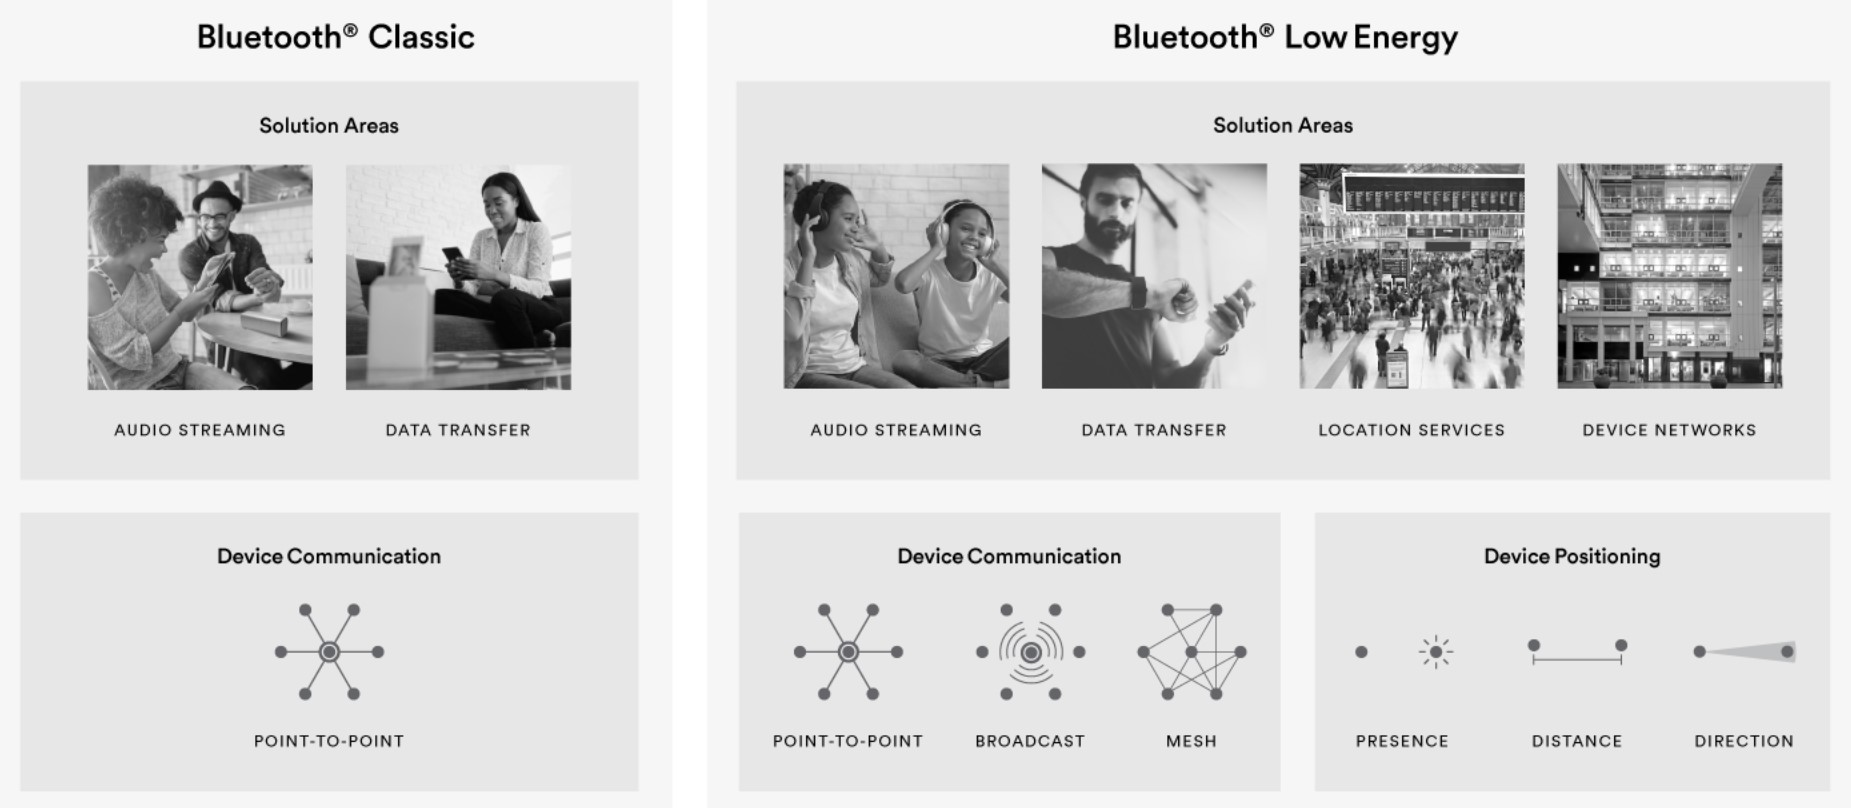
\includegraphics[width=\linewidth]{images/蓝牙}
    \end{figure}
\end{frame}


\begin{frame}[t]
    \frametitle{}
    \begin{block}{试一试：使用蓝牙功能分享一张图片给你的朋友}
        \begin{enumerate}
          \item 双方打开蓝牙
          \item 接收方：修改蓝牙名称为自己的名字
          \item 发送方：打开相册，选择一张照片，分享方式选择蓝牙
          \item 发送方：在蓝牙设备列表中找到你的朋友，发给他
          \item 接收方：收到蓝牙共享消息，选择“接受”
          \item 打开秒表，看看用蓝牙传输一张照片用时多久。
        \end{enumerate}
    \end{block}
\end{frame}


\begin{frame}
    \frametitle{蓝牙技术发展史}
    \begin{center}
        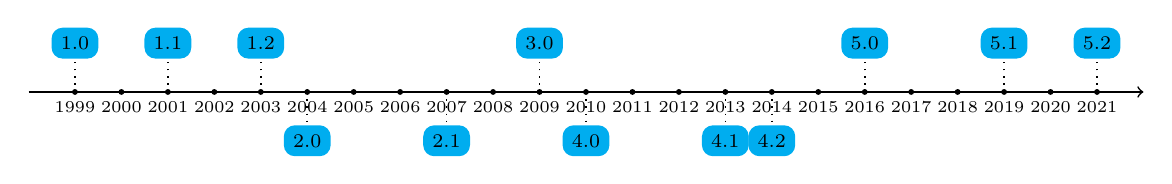
\begin{tikzpicture}[scale=0.59]
          \draw [->,semithick] (0,0) -- (24,0);
          \foreach \x [count=\i] in {1999,2000,2001,2002,2003,2004,2005,2006,2007,2008,2009,2010,2011,2012,2013,2014,2015,2016,2017,2018,2019,2020,2021}
          \filldraw ({\i},0) circle (.05) node [below,font=\fontsize{6}{6}\selectfont] {\x};
          \draw [dotted,semithick] (1,0) -- (1,0.7) node [above,rounded corners,rectangle,fill=cyan,font=\fontsize{7}{7}\selectfont] {1.0};
          \draw [dotted,semithick] (3,0) -- (3,0.7) node [above,rounded corners,rectangle,fill=cyan,font=\fontsize{7}{7}\selectfont] {1.1};
          \draw [dotted,semithick] (5,0) -- (5,0.7) node [above,rounded corners,rectangle,fill=cyan,font=\fontsize{7}{7}\selectfont] {1.2};
          \draw [dotted,semithick] (6,0) -- (6,-0.7) node [below,rounded corners,rectangle,fill=cyan,font=\fontsize{7}{7}\selectfont] {2.0};
          \draw [dotted,semithick] (9,0) -- (9,-0.7) node [below,rounded corners,rectangle,fill=cyan,font=\fontsize{7}{7}\selectfont] {2.1};
          \draw [dotted,semithick] (11,0) -- (11,0.7) node [above,rounded corners,rectangle,fill=cyan,font=\fontsize{7}{7}\selectfont] {3.0};
          \draw [dotted,semithick] (12,0) -- (12,-0.7) node [below,rounded corners,rectangle,fill=cyan,font=\fontsize{7}{7}\selectfont] {4.0};
          \draw [dotted,semithick] (15,0) -- (15,-0.7) node [below,rounded corners,rectangle,fill=cyan,font=\fontsize{7}{7}\selectfont] {4.1};
          \draw [dotted,semithick] (16,0) -- (16,-0.7) node [below,rounded corners,rectangle,fill=cyan,font=\fontsize{7}{7}\selectfont] {4.2};
          \draw [dotted,semithick] (18,0) -- (18,0.7) node [above,rounded corners,rectangle,fill=cyan,font=\fontsize{7}{7}\selectfont] {5.0};
          \draw [dotted,semithick] (21,0) -- (21,0.7) node [above,rounded corners,rectangle,fill=cyan,font=\fontsize{7}{7}\selectfont] {5.1};
          \draw [dotted,semithick] (23,0) -- (23,0.7) node [above,rounded corners,rectangle,fill=cyan,font=\fontsize{7}{7}\selectfont] {5.2};
      \end{tikzpicture}
      \end{center}
    \begin{table}
        \centering
        \begin{tabular}{cccc}
            \bottomrule
            蓝牙版本 & 最大传输速度 & 传输距离 &  \\ \hline
            蓝牙1 & 1\ Mbit/s & 10米 &  \\ 
            蓝牙2 & 3\ Mbit/s & 10米 &  \\ 
            蓝牙3 & 24\ Mbit/s & 10米 &  \\ 
            蓝牙4 & 48\ Mbit/s & 50米 &  \\ 
            蓝牙5 & 48\ Mbit/s & 300米 &  \\ \toprule
        \end{tabular}
    \end{table}
\end{frame}

% 蓝牙是一种短距离无线通信技术，它最初是为无线耳机设计的，但后来扩展到视频游戏控制器、打印机、扬声器等应用。目前有两种蓝牙版本，即经典蓝牙和蓝牙低功耗（BLE）。经典蓝牙（Bluetooth Classic）最初用于消费设备之间的点对点或点对多点（最多七个从属节点）的数据交换。后来，针对功耗进行优化，引入了蓝牙低功耗技术以此解决功耗敏感型的IoT应用需求。

% 支持BLE的IoT设备通常与智能设备（如智能手机）一起使用，在这里，智能手机主要负责向云端传输数据。现在，BLE被广泛集成到可穿戴设备（如智能手表、血糖仪、脉搏血氧仪等）以及智能家居设备（如门锁）中。

\begin{frame}
    \frametitle{蓝牙技术发展史}
    \begin{multicols}{2}
        \begin{enumerate}
          \item {\cbf{第一代蓝牙：短距离通讯早期探索}}
            \begin{itemize}
              \item {\bfseries 1.0} 从无到有
              \item {\bfseries 1.1} 列入 IEEE 802.15.1 标准
              \item {\bfseries 1.2} 改善抗干扰调频
            \end{itemize}
          \item {\cbf{第二代蓝牙：发力传输速率的时代}}
            \begin{itemize}
              \item {\bfseries 2.0} Enhanced Data Rate，3Mbps
              \item {\bfseries 2.1} 改善配对体验，支持NFC
            \end{itemize}
          \item {\cbf{第三代蓝牙：High Speed高速传输}}
            \begin{itemize}
              \item {\bfseries 3.0} 高速数据传输，达24Mbps 
            \end{itemize}
          \item {\cbf{第四代蓝牙：主推低功耗}}
            \begin{itemize}
              \item {\bfseries 4.0} BLE（Bluetooth Low Energy）
              \item {\bfseries 4.1} 支持与 LTE 无缝协作
              \item {\bfseries 4.2} 改善隐私保护
            \end{itemize}
          \item {\cbf{第五代蓝牙：开启物联网时代大门}}
            \begin{itemize}
              \item {\bfseries 5.0} 针对 IoT 物联网进行底层优化
              \item {\bfseries 5.1} 提高定位精度
              \item {\bfseries 5.2} LE功耗控制，LE同步信道
              \item {\bfseries 5.3} 提高LE通讯效率、降低功耗
            \end{itemize}
        \end{enumerate}
    \end{multicols}
\end{frame}


\begin{frame}[t]
    \frametitle{}
    \begin{question}
        蓝牙技术数据传输速度慢，容易受干扰，用户可能会遇到配对问题或连接蓝牙设备时遇到困难，连接设备数量有限……

        蓝牙缺点这么多，为什么还依然长盛不衰？
    \end{question}
\end{frame}


\begin{frame}
    \frametitle{$\vcenter{\hbox{
\includegraphics[height=14pt]{images/NearLinkB}}}$ NearLink 星闪 \link{http://sparklink.org.cn/news_info.php?id=669}}
    我们为何需要星闪？

    \begin{enumerate}
      \item 融合架构，一标多模
          \begin{itemize}
            \item SLB：对标Wi-Fi，应对高速率、大传输、高质量连接场景
            \item SLE：对标蓝牙，满足低功耗轻量级连接需求
          \end{itemize}
      \item 技术更先进、标准更领先、体验更突出
      \item 自主可控
    \end{enumerate}
    \begin{figure}[htpb]
      \centering
      
\includegraphics[width=\linewidth]{星闪优势}
    \end{figure}
\end{frame}


\begin{frame}
    \frametitle{$\vcenter{\hbox{
\includegraphics[height=14pt]{images/zigbee}}}$ Zigbee}
    \qquad Zigbee是一种新兴的低成本、低功耗的短距离无线通信协议，能够广泛的应用于军事、工业、智能家居等领域。但由于Zigbee技术出现较晚，其规范及应用仍在不断的完善和发展之中。

    \qquad Zigbee是基于IEEE802.15.4协议发展起来的一种短距离无线通信技术，功耗低，被业界认为是最有可能应用在工控场合的无线方式。ZigBee可工作在2.4GHz(全球流行)、868MHz(欧洲流行)和915 MHz(美国流行)3个频段上，分别具有最高250kbit/s、20kbit/s和40kbit/s的传输速率,它的传输距离在10-75m的范围内，但可以继续增加。
    \begin{multicols}{3}
        \begin{itemize}
          \item 低功耗
          \item 低成本
          \item 网络容量大
          \item 短时延
          \item 近距离
          \item 低速率
          \item 高安全
          \item 免执照频段
          \item 数据传输可靠
        \end{itemize}
    \end{multicols}
\end{frame}

\begin{frame}
  \frametitle{$\vcenter{\hbox{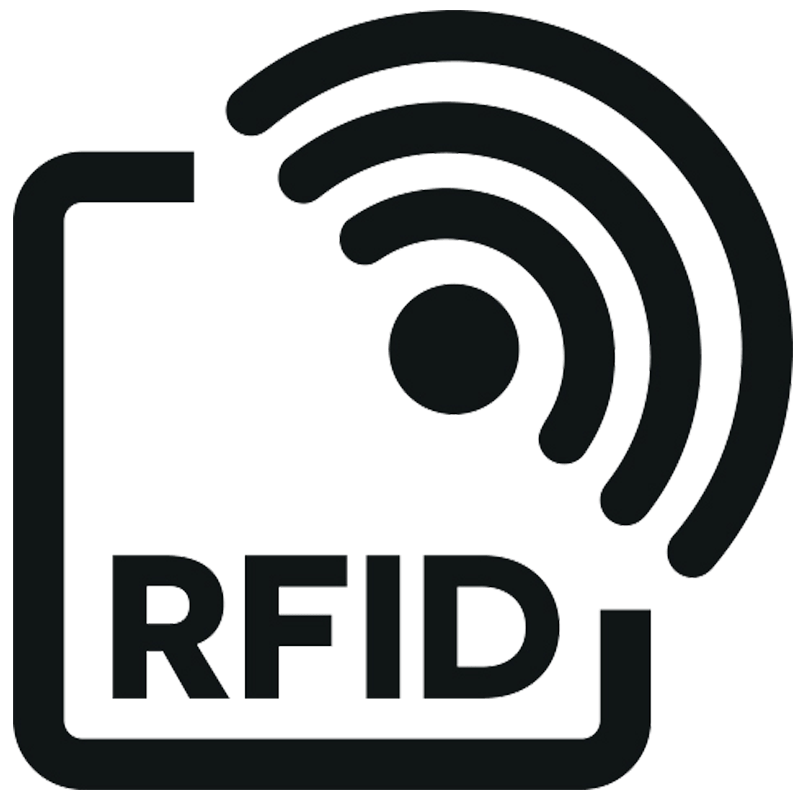
\includegraphics[height=14pt]{images/RFID}}}$ RFID 射频识别}
  射频识别（RFID）是一种无接触自动识别技术，利用射频信号在短距离内将少量数据从RFID标签传输到阅读器。RFID广泛应用于各种领域，从门禁控制到动物跟踪，从自动收费到供应链中的货物跟踪等。通过在各种产品和设备上贴上RFID标签，企业可以实时跟踪库存和资产，从而实现更好的库存和生产计划以及优化的供应链管理。

  \begin{figure}[htpb]
    \centering
    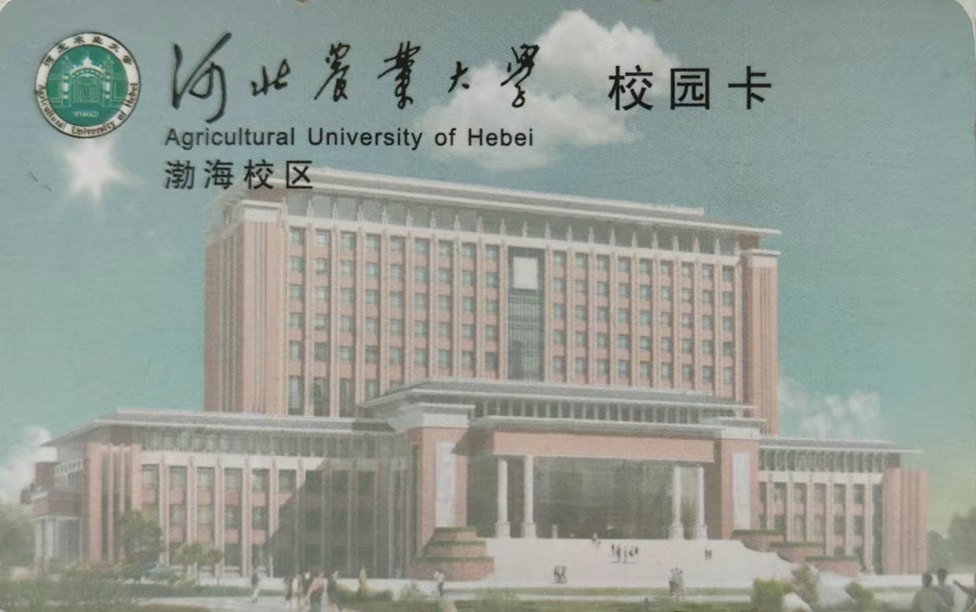
\includegraphics[width=.48\linewidth]{images/校园卡} \quad
    
\includegraphics[width=.48\linewidth]{images/公交卡}
\end{figure}
\end{frame}

\begin{frame}
  \frametitle{RFID系统的组成}
  RFID应用系统一般由读写器、标签和计算机系统等部分组成，有些简易的RFID系统则只是由读写器与标签组成。

  读写器和标签可以构成一个简单的应用系统，复杂的应用需要一个读写器同时读取n个标签，更复杂的应用系统则需要由计算机系统参与读取数据。

% 射频标签物理上由三部分组成：标签（tag）、天线、读写器。
% 标签(Tag)：由耦合元件及芯片组成，每个标签有唯一的电子编码，高容量电子标签有用户写入区，附着在物体上标识目标对象；
% 读写器(Reader)：读取(有时还可以写入)标签信息的设备，可设计为手持式或固定式；
% 天线(Antenna)：在标签和读取器间传递射频信号。

  \begin{figure}[htpb]
    \centering
    
\includegraphics[width=\linewidth]{RFID组成}
  \end{figure}
\end{frame}

\begin{frame}
  \frametitle{RFID系统的基本工作原理}
  \begin{enumerate}
    \item 由阅读器通过发射天线发送特定频率的射频信号，当电子标签进入有效工作区域时产生感应电流，从而获得能量、电子标签被激活，使得电子标签将自身编码信息通过内置射频天线发送出去；
    \item 阅读器的接收天线接收到从标签发送来的调制信号，经天线调节器传送到阅读器信号处理模块，经解调和解码后将有效信息送至后台主机系统进行相关的处理；
  \end{enumerate}
    \begin{minipage}{0.38\linewidth}
          \begin{itemize}
            \item[3.]主机系统根据逻辑运算识别该标签的身份，针对不同的设定作出相应的处理和控制，最终发出指令信号控制阅读器完成相应的读写操作。
          \end{itemize}
      \end{minipage}\hfill
      \begin{minipage}{0.58\linewidth}
        \begin{figure}[htpb]
          \centering
          
\includegraphics[width=.9\linewidth]{RFID原理}
        \end{figure}
      \end{minipage}

\end{frame}

\begin{frame}
    \frametitle{RFID工作频率}
    \begin{itemize}
      \item \cbf{低频(LF)}
      
      30KHz – 300KHz, 典型的工作频率有125kHz、225kHz
      
      电子标签的成本较低、标签内保存的数据量较少、阅读距离较短(小于10cm)

      典型应用有：动物识别、容器识别、工具识别、门禁和安全管理系统。
      \item \cbf{高频(HF)}
      
      3MHz – 30MHz, 典型的工作频率有13.56MHz
      
      读取距离一般小于1米，数据传输速率较高
      \item \cbf{超高频(UHF)/微波}
      
      > 300MHz，典型的工作频段有915MHz、2.45GHz、5.8GHz

      电子标签及读写器成本较高、标签内保存的数据量较大、阅读距离较远（可达几米至十几米），适应物体高速运动性能好。

      典型应用包括：移动车辆识别、仓储物流管理和应用
    \end{itemize}
\end{frame}


\begin{frame}
    \frametitle{RFID技术在农业中的应用：智慧养殖}
    通过RFID技术对奶牛的身份信息进行识别，通过姿态传感器可以检测奶牛的行为，包括进食、排泄、分娩、休息。同时可有在牛的饲料装置下加入压力传感器，从而可以检测出奶牛的进食量。
    \begin{figure}[htpb]
        \centering
        
\includegraphics[height=.25\linewidth]{奶牛RFID}
        
\includegraphics[height=.25\linewidth]{奶牛传感器}
    \end{figure}
\end{frame}


\begin{frame}
    \frametitle{支付宝“碰一碰”支付\link{https://36kr.com/p/2855558959057794}}
    \begin{figure}[htpb]
        \centering
        
\includegraphics[width=\linewidth]{碰一碰}
    \end{figure}
\end{frame}


\begin{frame}
  \frametitle{$\vcenter{\hbox{
\includegraphics[height=13pt]{images/nfc}}}$ NFC 近场通信}
    \begin{minipage}{0.38\linewidth}
      NFC是在RFID基础上发展而来的，增加了点对点通信功能，可以快速建立蓝牙设备之间的P2P（点对点）无线通信。
      
      NFC可以理解为RFID技术的一个子集，使用的是13.56MHz频段。      
      \end{minipage}\hfill
      \begin{minipage}{0.58\linewidth}
        \begin{figure}[htpb]
          \centering
          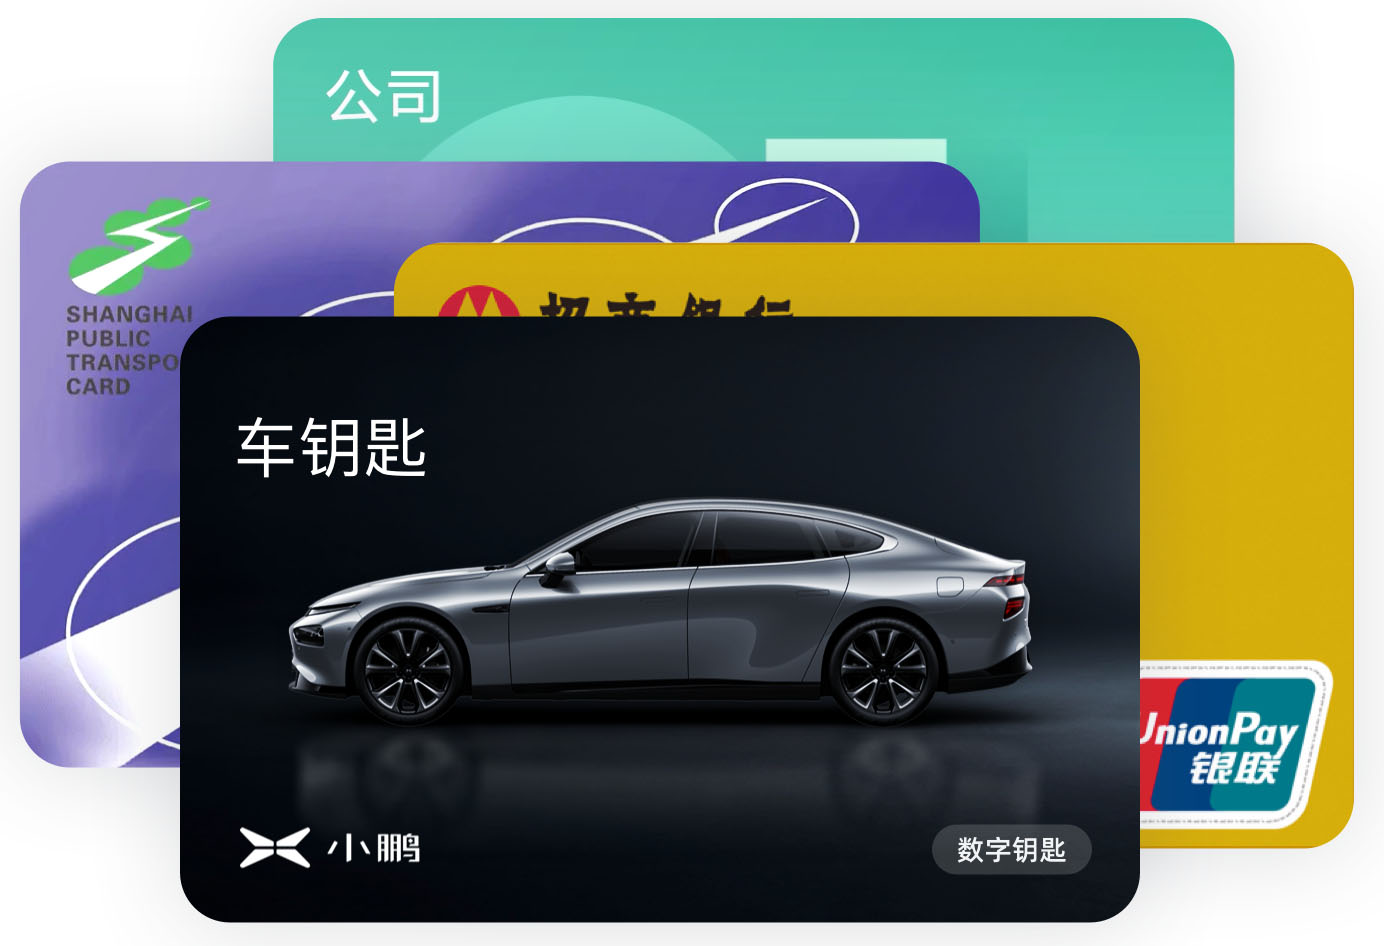
\includegraphics[width=\linewidth]{images/NFC卡}
        \end{figure}
      \end{minipage}
\end{frame}


\begin{frame}
    \frametitle{}
    \begin{block}{小调查：你最常用的手机支付方式是？}
        \begin{itemize}
          \item[A：] 支付宝
          \item[B：] 微信
          \item[C：] 其他
        \end{itemize}
    \end{block}
\end{frame}


\begin{frame}
    \frametitle{$\vcenter{\hbox{
\includegraphics[height=14pt]{images/UWB}}}$ UWB 超宽带通信}
    \emph{一些技术的真正实用价值，有时需要多年以后才能得到体现。}

    曾经UWB被认定会成为“短距离无线传输”领域的主流技术，但最终没有“卷”过WiFi和BLE蓝牙技术。在消费级市场领域遇冷10多年后，随着技术标准的不断完善，还有苹果等消费电子大厂加持，UWB重新回到了大家的视野中。
    \bigskip

      \begin{minipage}{0.48\linewidth}
            \begin{figure}[htpb]
              \centering
              {\bfseries 定位精度高}
              \smallskip

              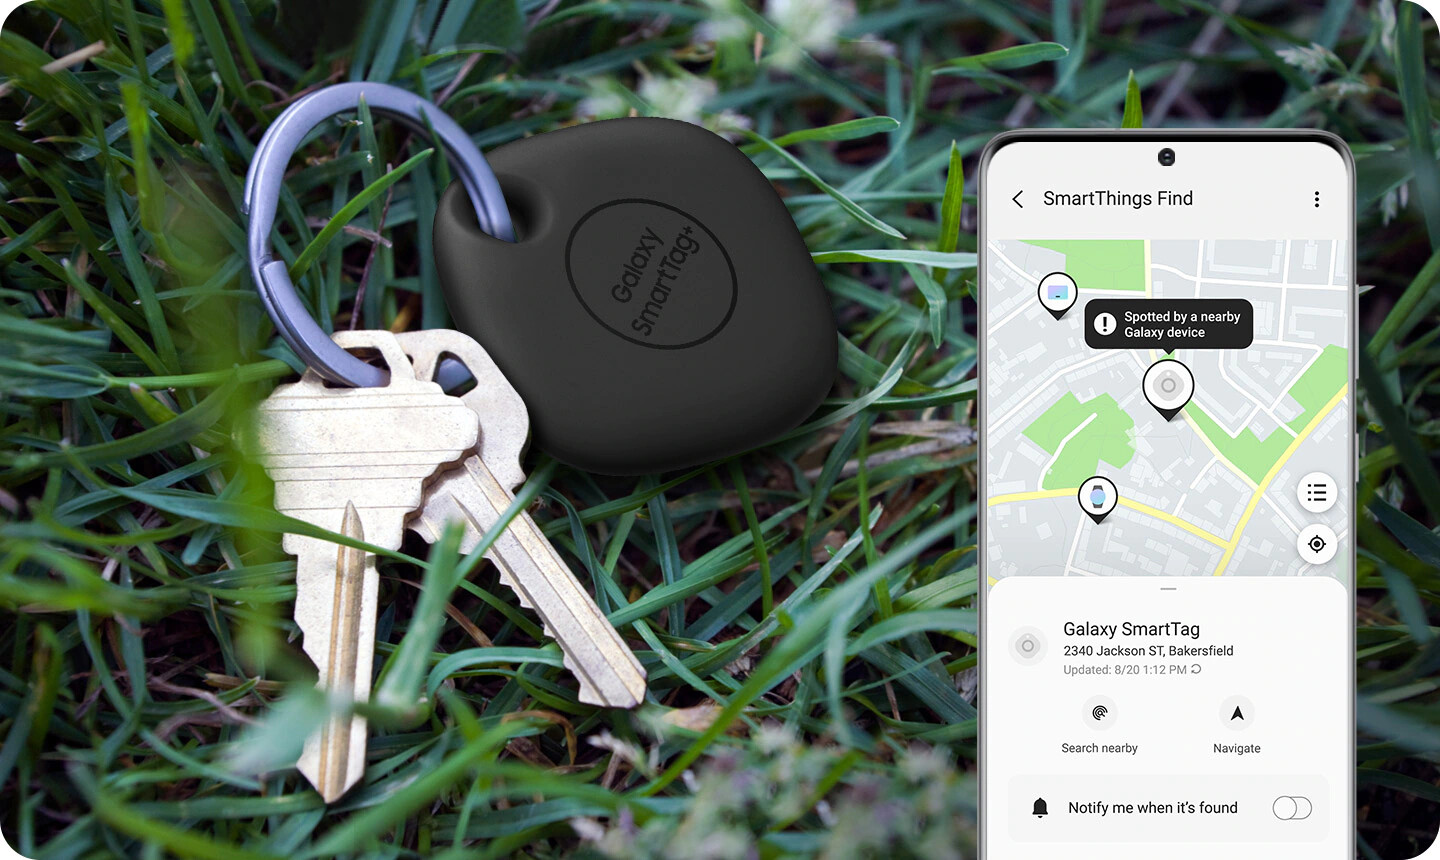
\includegraphics[height=.5\linewidth]{images/smarttag+}
            \end{figure}
        \end{minipage}\hfill
        \begin{minipage}{0.48\linewidth}
          \begin{figure}[htpb]
            \centering
            {\bfseries 传输速率高}
            \smallskip

            
\includegraphics[height=.5\linewidth]{images/隔空投送}
          \end{figure}
        \end{minipage}
\end{frame}


\begin{frame}
    \frametitle{汽车数字钥匙}
    数字钥匙采用NFC、BLE（蓝牙）、UWB通信技术，将NFC智能卡、智能手机、智能手表和智能手环等智能终端设备变成车钥匙，从而实现无钥匙进入和启动、为他人远程钥匙授权、个性化的车辆设置等便捷功能。
    \begin{itemize}
      \item {\bfseries 第一代数字钥匙} \quad 基于NFC
      
      基本没有位置感知的能力。车主需要将数字钥匙贴近车身才能开启车门。
      \item {\bfseries 第二代数字钥匙} \quad NFC+BLE
      
      通信距离比第一代更远。可以通过蓝牙信号的强弱粗略感知车与钥匙的位置关系，但其感知精度与准确性都有所欠缺。
      \item {\bfseries 第三代数字钥匙} \quad NFC+BLE+UWB
      
      位置感知精度得到了质的飞跃。极大地提升了数字钥匙的安全性。
    \end{itemize}
\end{frame}

% https://zhuanlan.zhihu.com/p/458294241

% https://zhuanlan.zhihu.com/p/180082384

% 智能钥匙系统采用无线射频识别（RFID）技术，通常情况下，当车主走近车辆大约一米以内距离时，门锁就会自动打开并解除防盗；当离开车辆时，门锁会自动锁上并进入防盗状态。当车主进入车内时，车内检测系统会马上识别智能卡，这时只需轻轻按动启动按钮(或旋钮)，就可以正常启动车辆，整个过程，车钥匙无须拿出。

% 常规的无钥匙解锁的过程中，大概是这样的：钥匙会给车子发送一个信号，然后车子会和实体钥匙 or 手机钥匙发过来的信号进行确认，然后解锁车辆。

% 但是需要注意的是，大多数无钥匙进入系统只是通过信号强度来确定车辆驾驶员是否在范围内。也就是说，只要把这个沟通过程的信号放大，使得车子和钥匙「以为」车主就在附近，即可完成解锁操作。

% 这就产生了一种攻击方式：中继站攻击。比如说，我在家睡觉，钥匙就在旁边，靠近车辆的小偷会拉门把手假装开车门，然后通过手中的中继站收集来自车辆的请求解锁信号，这个信息会发送到靠近我身边钥匙的另外一个人的中继站里，而后发射到钥匙里，钥匙在收到信号后会返回一个有效信号，通过两个中继站回传到车内。中继站的作用就是放大了车子和钥匙沟通的信号强度，使得车子和钥匙「以为」车主就在车旁边，然后完成解锁动作，小偷就这样把车偷走了。

% UWB计算距离使用的原理是飞行时间（ToF），即发送端发射一个信号，接收端在收到这个信号之后经过协议定义的延迟后再发回给发送端，这样发送端只要比较发送和接受信号的时间差并乘以光速就能获得发送端与接收端之间的距离，从而可以实现亚米级别的距离精度。

% 通过这种高精度的定位，系统会通过钥匙到车子的信号传递时间来计算用户与车子的距离，如果窃贼想要通过中继站增强信号来获得开门权限，当系统探测到用户到车子的距离超出钥匙控车的最远距离，即会判定这是一次攻击，不会开启车门。

% 可以有效避免中继站攻击，对于追求安全的车厂们来说，很有吸引力，而且，当手机上拥有 UWB、蓝牙和 NFC 三个功能时，可以为用户提供更安全且精准的无钥匙进入体验：使用蓝牙唤醒 UWB，加密传输数据功能，UWB 则用于精准定位，而 NFC 则是用于手机没电情况下的备用进入手段。

\begin{frame}
    \frametitle{$\vcenter{\hbox{
\includegraphics[height=14pt]{images/nbiot}}}$ NB-IoT 窄带物联网}
    NB-IoT是基于蜂窝网络的窄带物联网。

    特点是广覆盖、大规模、低功耗、低成本。
    % 在4G技术定义初期，并没有把物联网的需求纳入考虑，因此业界后来又发展出NB-IoT，以补上这个缺口。 5G则与4G不同，在标准定义初期，就把物联网应用的需求纳入考虑，并制定出对应的mMTC技术标准。 不过，目前还很难断言mMTC是否会完全取代NB-IoT，因为mMTC与NB-IoT虽然在应用领域有所重迭，但mMTC会具备一些NB-IoT所没有的特性，反之亦然。 像是极低的网络等待时间，就是NB-IoT所没有的特性。

    \begin{figure}[htpb]
      \centering
      
\includegraphics[width=.8\linewidth]{NB-IOT}
    \end{figure}
\end{frame}

\begin{frame}
  \frametitle{mMTC}
  mMTC 是 5G 应用最为广泛的三大重要场景之一，专为物联网而生。
    \begin{minipage}{0.38\linewidth}
          \begin{center}
            \bf{5G三大应用场景：}
            \bigskip

              \begin{tikzpicture}
                \draw [rounded corners,fill=LightCyan1] (0,0) rectangle (5,1) node [midway] {mMTC 海量物联网通信};
                \draw [rounded corners,fill=LightCyan1,shift={(0,1.2)}] (0,0) rectangle (5,1) node [midway] {uRLLC 高可靠低时延通信};
                \draw [rounded corners,fill=LightCyan1,shift={(0,2.4)}] (0,0) rectangle (5,1) node [midway] {eMBB 增强移动宽带};
              \end{tikzpicture}
          \end{center}
      \end{minipage}\hfill
      \begin{minipage}{0.58\linewidth}
        \vspace{1em}
        \begin{itemize}
          \item 一平方公里内，能够承载100万个终端；
          \item 最差的信号环境下，时延小于10s；
          \item 最差信号环境下，电池寿命大于十年。
        \end{itemize}
        \begin{figure}[htpb]
          \centering
          
\includegraphics[width=.7\linewidth]{智慧城市}
        \end{figure}
      \end{minipage}
\end{frame}

%   5G的三大业务场景eMBB、URLLC、mMTC：

%  eMBB：英文全称Enhanced Mobile Broadband，即增强移动宽带，是利用5G更好的网络覆盖及更高的传输速率来为用户提供更好的上网接入服务，使得无线上网具有更高的上网速率和更稳定的传输，给客户带来的最直观的感受就是网速的大幅提升，即便是观看 4K 高清视频，峰值能够达到 10Gbps。

%  URLLC：英文全称Ultra Reliable & LowLatency Communication，即低时延高可靠，如名称所述，URLLC有两个基本特点，即高可靠和低时延，可以广泛应用于如AR/VR、工业控制系统、交通和运输（如无人驾驶）、智能电网和智能家居的管理、交互式的远程医疗诊断等。

%  mMTC：英文全称Massive Machine Type Communication，即海量物联网通信或大规模物联网业务，5G 低功耗、大连接和低时延高可靠的特性很好地适应了面向物联网的业务，可以重点解决传统移动通信无法很好支持地物联网及垂直行业应用。低功耗大连接场景主要面向智慧城市、环境监测、智能农业、森林防火等以传感和数据采集为目标的应用场景，具有小数据包、低功耗、海量连接等特点。这类终端分布范围广、数量众多，不仅要求网络具备超千亿连接的支持能力，满足 100 万 /km2 连接数密度指标要求，而且还要保证终端的超低功耗和超低成本。

\begin{frame}
    \frametitle{$\vcenter{\hbox{
\includegraphics[height=14pt]{images/lora}}}$ Lora}
      \begin{minipage}{0.32\linewidth}
        \bf{物联网的无线通信技术：}
        \begin{itemize}
          \item 短距离通信技术
            \begin{itemize}
              \item WiFi
              \item 蓝牙
              \item Zigbee等
            \end{itemize}
          \item 广域网通信技术
            \begin{itemize}
              \item NB-IoT
              \item LoRa
            \end{itemize}
        \end{itemize}
      \end{minipage}\hfill
      \begin{minipage}{0.65\linewidth}
        LoRa和NB-IoT的技术特点非常相似，都是低功耗、广覆盖，适合海量连接场景。其最主要的不同就是，NB-IoT是运营商建网和提供服务，而LoRa是自建网络。

        \begin{itemize}
          \item[\bf{优势}] 自组网络。企业可以自主运营，可以把运营数据掌握在自己手中；自主把控网络质量，根据业务需要扩展网络，对网络覆盖可快速优化补充。
          \item[\bf{风险}] LoRa技术中，LoRa芯片处在整个产业链中处于基础核心地位，目前美国Semtech公司是LoRa芯片的核心供应商，掌握着LoRa底层技术的核心专利。
        \end{itemize}
      \end{minipage}
\end{frame}

\begin{frame}
    \frametitle{无线通信技术对比}
\begin{table}[]
    \begin{tabular}{@{}cll@{}}
    \toprule
           & \multicolumn{1}{c}{优点} & \multicolumn{1}{c}{缺点} \\ \midrule
    蓝牙     & 功耗低，便宜，延时低             & 容易受到信号干扰，联网耗时较久        \\
    WiFi   & 传输速率高                  & 信号覆盖范围有限，功耗大           \\
    Zigbee & 容量大，安全性高，功耗低           & 传输距离短，传输速率受限           \\
    Lora   & 传输距离远，穿透障碍物能力较强        & 速率低，传输时延较大             \\
    NB-IoT & 覆盖超强，海量接入，低功耗，低成本      & 速率较低，成本高               \\
    4G     & 传输速度更快，网络延迟更低          & 成本高，更高的能源消耗            \\ \bottomrule
    \end{tabular}
    \end{table}
\end{frame}

\begin{frame}
    \frametitle{如何选择最适合的物联网无线技术？}
    物联网应用中有许多优秀的无线通信技术。然而，没有一种技术是面面俱到的。要选择合适的物联网无线技术，需要根据具体需求来评估，在功耗、数据范围和带宽之间进行权衡，同时还要考虑电池大小、成本、传输距离以及固件更新等因素。
    \begin{itemize}
      \item 您需要传输多少数据？
      \item 需要的功率是多少？
      \item 数据源离互联网有多远？
      \item 服务费用有多高？
      \item 这些设备将在哪里使用？
    \end{itemize}
\end{frame}


\begin{frame}[t]
    \frametitle{}
    \begin{block}{选择任一话题进行思考讨论}
        \begin{enumerate}
          \item 探讨物联网技术的应用
          \item 同学们接触过哪些物联网设备？它使用了什么技术？
          \item 你认为物联网技术在农业中可以起到什么作用？
          \item 为什么物联网无线接入技术对农业物联网的应用非常关键？
          \item 为什么NFC这样一个看起来、用起来都要比二维码更好的技术始终未能得到普及？
          \item 你认为未来的移动支付会是什么样子的？
          \item 微信圆形的小程序码，属于QR码吗？
        \end{enumerate}
    \end{block}
\end{frame}





\end{document}
